\newpage

\subsection{Principales datos socio-demográficos del IPS}

\subsubsection{Indicadores anuales de los trabajadores activos cotizantes al fondo de jubilaciones (personas)}

Cabe mencionar que es necesario asumir una definición concreta del
trabajador activo para generar las estadísticas. Para los fines
específicos del Informe Actuarial se considera como trabajador activo
cotizante al Fondo de Jubilaciones y Pensiones en un año determinado, a
todo trabajador que figure en la base de datos. Las bases de datos (BD)
de la DAOP son dinámicas, en el sentido que las cantidades pueden ir
modificándose a medida que se actualizan o adicionan datos que
generalmente corresponden a p agos (aportes) que se realizan con cierta
demora o atrasos. En este caso particular, la BD utilizada fue generada
en fecha 22/05/2018. Las cifras pueden presentar diferencias con las
publicadas por la DIPLAN en sus anuarios debido a la fecha de corte pa
ra la obtención de estas o bien debido a las distintas definiciones
utilizadas para generar las estadísticas.
\footnote{Las bases de datos (BD) de la DAOP son dinámicas, en el sentido que las cantidades pueden ir modificándose a medida que se actualizan
 o adicionan datos que generalmente corresponden a pagos (aportes) que se realizan con cierta demora o atrasos. En este caso particular, la BD utilizada fue generada en fecha 22/05/2018. Las cifras pueden presentar diferencias con las publicadas por la 
DIPLAN en sus anuarios debido a la fecha de corte para la obtención de estas o bien debido a las distintas definiciones utilizadas para generar las estadísticas.}
con al menos un aporte registrado en dicho año. Las cantidades de
activos y los salarios c orresponden a la planilla de pagos del mes de
enero a diciembre del año 2020, de acuerdo al mes en el cual se haya
registrado el último
aporte\footnote{Del total de cotizantes registrados a la fecha de consulta de la base},
se registraron 580.524 cotiza ntes en el mes de enero, para diciembre
presentaron cotización 547.571 personas, marcando así una disminución de
cotizantes al termino del año en un 5.68\% . Para dicho año, el IPS
contaba con 712.309 activos cotizantes del Fondo de J y P de 15 y más
años de edad, de los cuales 258.003 (36,22\%) eran mujeres y 454.306
hombres (63,78\%). El grupo más numeroso se encontraba en la franja
etaria comprendida entre los 20 y 41 años.

\textbf{Características de los cotizantes en el año 2020}

\begin{table}[H]
\begin{center}
\scriptsize
\caption{\bf{Cantidad de cotizantes por edades, según año (Personas)}}
\begin{tabular}{l|rrrrrrrrrrrrr}
\textbf{edadtop} & \multicolumn{2}{c}{\textbf{Hombres}} & \multicolumn{2}{c}{\textbf{Mujeres}} & \multicolumn{2}{c}{\textbf{Total}} \\
&Cant.&Porc.&Cant.&Porc.&Cant.&Porc. \\
\hline
18 y menos&4.353&0,96\%&1.737&0,67\%&6.090&0,85\% \\
19&8.247&1,82\%&3.751&1,45\%&11.998&1,68\% \\
20&11.318&2,49\%&6.069&2,35\%&17.387&2,44\% \\
21&13.836&3,05\%&7.728&3,00\%&21.564&3,03\% \\
22&15.253&3,36\%&9.140&3,54\%&24.393&3,42\% \\
23&17.075&3,76\%&10.295&3,99\%&27.370&3,84\% \\
24&17.865&3,93\%&11.424&4,43\%&29.289&4,11\% \\
25&17.935&3,95\%&11.428&4,43\%&29.363&4,12\% \\
26&18.150&4,00\%&11.646&4,51\%&29.796&4,18\% \\
27&18.170&4,00\%&11.782&4,57\%&29.952&4,20\% \\
28&18.243&4,02\%&11.576&4,49\%&29.819&4,19\% \\
29&17.993&3,96\%&11.460&4,44\%&29.453&4,13\% \\
30&17.176&3,78\%&10.636&4,12\%&27.812&3,90\% \\
31&16.613&3,66\%&10.049&3,89\%&26.662&3,74\% \\
32&15.591&3,43\%&9.352&3,62\%&24.943&3,50\% \\
33&14.744&3,25\%&8.608&3,34\%&23.352&3,28\% \\
34&14.162&3,12\%&8.354&3,24\%&22.516&3,16\% \\
35&13.733&3,02\%&7.785&3,02\%&21.518&3,02\% \\
36&13.754&3,03\%&7.680&2,98\%&21.434&3,01\% \\
37&13.091&2,88\%&7.147&2,77\%&20.238&2,84\% \\
38&12.610&2,78\%&7.060&2,74\%&19.670&2,76\% \\
39&11.306&2,49\%&6.224&2,41\%&17.530&2,46\% \\
40&10.909&2,40\%&5.942&2,30\%&16.851&2,37\% \\
41&9.760&2,15\%&5.028&1,95\%&14.788&2,08\% \\
42&8.501&1,87\%&4.632&1,80\%&13.133&1,84\% \\
43&7.973&1,75\%&4.080&1,58\%&12.053&1,69\% \\
44&7.322&1,61\%&3.789&1,47\%&11.111&1,56\% \\
45&6.834&1,50\%&3.489&1,35\%&10.323&1,45\% \\
46&6.382&1,40\%&3.282&1,27\%&9.664&1,36\% \\
47&5.942&1,31\%&2.976&1,15\%&8.918&1,25\% \\
48&5.893&1,30\%&2.906&1,13\%&8.799&1,24\% \\
49&5.530&1,22\%&2.791&1,08\%&8.321&1,17\% \\
50&5.404&1,19\%&2.621&1,02\%&8.025&1,13\% \\
51&5.062&1,11\%&2.431&0,94\%&7.493&1,05\% \\
52&4.817&1,06\%&2.407&0,93\%&7.224&1,01\% \\
53&4.360&0,96\%&2.121&0,82\%&6.481&0,91\% \\
54&4.400&0,97\%&2.085&0,81\%&6.485&0,91\% \\
55&4.158&0,92\%&2.006&0,78\%&6.164&0,87\% \\
56&3.762&0,83\%&1.828&0,71\%&5.590&0,78\% \\
57&3.593&0,79\%&1.700&0,66\%&5.293&0,74\% \\
58&3.200&0,70\%&1.516&0,59\%&4.716&0,66\% \\
59&3.342&0,74\%&1.667&0,65\%&5.009&0,70\% \\
60&2.676&0,59\%&1.266&0,49\%&3.942&0,55\% \\
61&2.078&0,46\%&986&0,38\%&3.064&0,43\% \\
62&1.814&0,40\%&841&0,33\%&2.655&0,37\% \\
63&1.686&0,37\%&748&0,29\%&2.434&0,34\% \\
64&1.662&0,37\%&705&0,27\%&2.367&0,33\% \\
65&1.270&0,28\%&541&0,21\%&1.811&0,25\% \\
66&849&0,19\%&504&0,20\%&1.353&0,19\% \\
67&726&0,16\%&373&0,14\%&1.099&0,15\% \\
68&604&0,13\%&288&0,11\%&892&0,13\% \\
69&477&0,10\%&226&0,09\%&703&0,10\% \\
70 y más&2.102&0,46\%&1.297&0,50\%&3.399&0,48\% \\
\textbf{Total}&454.306&100,00\%&258.003&100,00\%&712.309&100,00\% \\

\end{tabular}
                            \item Fuente : Elaboración própia a partir de registros administrativos del IPS.
\end{center}
\end{table}

\begin{figure}[H]
\begin{center}
                    \caption{Distribución de la cantidad de personas cotizantes al FJ por edad y sexo}
                    \vspace{0.5cm}
                    \includegraphics[scale=0.4]{RA_IPS_cotizantes_2020_sexo_edad_18a70.png}
\end{center}
\end{figure}

\begin{table}[H]
\begin{center}
\scriptsize
\caption{\bf{Distribución de la cantidad de personas cotizantes al FJ por tramos de edad y sexo}}
\begin{tabular}{l|rrrrrrrrrrrrr}
\input{RA_IPS_cotizantes_2020_sexo_edadt_18a70}
\end{tabular}
                    \item Fuente : Elaboración própia a partir de registros administrativos del IPS.
\end{center}
\end{table}

\begin{figure}[H]
\begin{center}
                    \caption{Pirámide de población - (Cotizantes. Año 2020)}
                    \vspace{0.5cm}
                    \includegraphics[scale=0.6]{RA_IPS_cotizantes_2020_sexo_edadt_piramide.png}
\end{center}
\end{figure}

\begin{table}[H]
\begin{center}
\scriptsize
\caption{\bf{Salario promedio de las personas cotizantes al FJ por edad y sexo}}
\begin{tabular}{l|rrrrrrrrrrrrr}
\begin{tabular}{llll}
\cline{1-4}
\multicolumn{1}{c}{} &
  \multicolumn{3}{|c}{Sexo} \\
\multicolumn{1}{c}{} &
  \multicolumn{1}{|r}{Hombres} &
  \multicolumn{1}{r}{Mujeres} &
  \multicolumn{1}{r}{Total} \\
\cline{1-4}
\multicolumn{1}{l}{Edad} &
  \multicolumn{1}{|r}{} &
  \multicolumn{1}{r}{} &
  \multicolumn{1}{r}{} \\
\multicolumn{1}{l}{\hspace{1em}18 y menos} &
  \multicolumn{1}{|r}{1.647.398} &
  \multicolumn{1}{r}{1.573.401} &
  \multicolumn{1}{r}{1.647.398} \\
\multicolumn{1}{l}{\hspace{1em}19} &
  \multicolumn{1}{|r}{1.869.872} &
  \multicolumn{1}{r}{1.831.838} &
  \multicolumn{1}{r}{1.869.872} \\
\multicolumn{1}{l}{\hspace{1em}20} &
  \multicolumn{1}{|r}{2.057.655} &
  \multicolumn{1}{r}{2.044.521} &
  \multicolumn{1}{r}{2.057.655} \\
\multicolumn{1}{l}{\hspace{1em}21} &
  \multicolumn{1}{|r}{2.199.210} &
  \multicolumn{1}{r}{2.161.953} &
  \multicolumn{1}{r}{2.199.210} \\
\multicolumn{1}{l}{\hspace{1em}22} &
  \multicolumn{1}{|r}{2.295.259} &
  \multicolumn{1}{r}{2.251.440} &
  \multicolumn{1}{r}{2.295.259} \\
\multicolumn{1}{l}{\hspace{1em}23} &
  \multicolumn{1}{|r}{2.415.027} &
  \multicolumn{1}{r}{2.386.680} &
  \multicolumn{1}{r}{2.415.027} \\
\multicolumn{1}{l}{\hspace{1em}24} &
  \multicolumn{1}{|r}{2.539.971} &
  \multicolumn{1}{r}{2.520.227} &
  \multicolumn{1}{r}{2.539.971} \\
\multicolumn{1}{l}{\hspace{1em}25} &
  \multicolumn{1}{|r}{2.675.760} &
  \multicolumn{1}{r}{2.681.596} &
  \multicolumn{1}{r}{2.681.596} \\
\multicolumn{1}{l}{\hspace{1em}26} &
  \multicolumn{1}{|r}{2.868.071} &
  \multicolumn{1}{r}{2.836.183} &
  \multicolumn{1}{r}{2.868.071} \\
\multicolumn{1}{l}{\hspace{1em}27} &
  \multicolumn{1}{|r}{2.972.912} &
  \multicolumn{1}{r}{3.000.978} &
  \multicolumn{1}{r}{3.000.978} \\
\multicolumn{1}{l}{\hspace{1em}28} &
  \multicolumn{1}{|r}{3.095.174} &
  \multicolumn{1}{r}{3.084.374} &
  \multicolumn{1}{r}{3.095.174} \\
\multicolumn{1}{l}{\hspace{1em}29} &
  \multicolumn{1}{|r}{3.252.230} &
  \multicolumn{1}{r}{3.200.132} &
  \multicolumn{1}{r}{3.252.230} \\
\multicolumn{1}{l}{\hspace{1em}30} &
  \multicolumn{1}{|r}{3.384.950} &
  \multicolumn{1}{r}{3.335.319} &
  \multicolumn{1}{r}{3.384.950} \\
\multicolumn{1}{l}{\hspace{1em}31} &
  \multicolumn{1}{|r}{3.554.837} &
  \multicolumn{1}{r}{3.446.023} &
  \multicolumn{1}{r}{3.554.837} \\
\multicolumn{1}{l}{\hspace{1em}32} &
  \multicolumn{1}{|r}{3.643.920} &
  \multicolumn{1}{r}{3.641.841} &
  \multicolumn{1}{r}{3.643.920} \\
\multicolumn{1}{l}{\hspace{1em}33} &
  \multicolumn{1}{|r}{3.705.939} &
  \multicolumn{1}{r}{3.671.003} &
  \multicolumn{1}{r}{3.705.939} \\
\multicolumn{1}{l}{\hspace{1em}34} &
  \multicolumn{1}{|r}{3.888.751} &
  \multicolumn{1}{r}{3.738.498} &
  \multicolumn{1}{r}{3.888.751} \\
\multicolumn{1}{l}{\hspace{1em}35} &
  \multicolumn{1}{|r}{3.965.026} &
  \multicolumn{1}{r}{3.825.647} &
  \multicolumn{1}{r}{3.965.026} \\
\multicolumn{1}{l}{\hspace{1em}36} &
  \multicolumn{1}{|r}{3.996.414} &
  \multicolumn{1}{r}{3.900.499} &
  \multicolumn{1}{r}{3.996.414} \\
\multicolumn{1}{l}{\hspace{1em}37} &
  \multicolumn{1}{|r}{4.055.798} &
  \multicolumn{1}{r}{3.892.665} &
  \multicolumn{1}{r}{4.055.798} \\
\multicolumn{1}{l}{\hspace{1em}38} &
  \multicolumn{1}{|r}{4.154.389} &
  \multicolumn{1}{r}{3.949.822} &
  \multicolumn{1}{r}{4.154.389} \\
\multicolumn{1}{l}{\hspace{1em}39} &
  \multicolumn{1}{|r}{4.210.606} &
  \multicolumn{1}{r}{3.994.473} &
  \multicolumn{1}{r}{4.210.606} \\
\multicolumn{1}{l}{\hspace{1em}40} &
  \multicolumn{1}{|r}{4.179.287} &
  \multicolumn{1}{r}{4.003.800} &
  \multicolumn{1}{r}{4.179.287} \\
\multicolumn{1}{l}{\hspace{1em}41} &
  \multicolumn{1}{|r}{4.145.900} &
  \multicolumn{1}{r}{3.912.505} &
  \multicolumn{1}{r}{4.145.900} \\
\multicolumn{1}{l}{\hspace{1em}42} &
  \multicolumn{1}{|r}{4.335.325} &
  \multicolumn{1}{r}{3.977.352} &
  \multicolumn{1}{r}{4.335.325} \\
\multicolumn{1}{l}{\hspace{1em}43} &
  \multicolumn{1}{|r}{4.218.473} &
  \multicolumn{1}{r}{3.853.365} &
  \multicolumn{1}{r}{4.218.473} \\
\multicolumn{1}{l}{\hspace{1em}44} &
  \multicolumn{1}{|r}{4.390.030} &
  \multicolumn{1}{r}{3.978.599} &
  \multicolumn{1}{r}{4.390.030} \\
\multicolumn{1}{l}{\hspace{1em}45} &
  \multicolumn{1}{|r}{4.173.082} &
  \multicolumn{1}{r}{3.955.129} &
  \multicolumn{1}{r}{4.173.082} \\
\multicolumn{1}{l}{\hspace{1em}46} &
  \multicolumn{1}{|r}{4.199.792} &
  \multicolumn{1}{r}{3.830.997} &
  \multicolumn{1}{r}{4.199.792} \\
\multicolumn{1}{l}{\hspace{1em}47} &
  \multicolumn{1}{|r}{4.223.070} &
  \multicolumn{1}{r}{3.895.532} &
  \multicolumn{1}{r}{4.223.070} \\
\multicolumn{1}{l}{\hspace{1em}48} &
  \multicolumn{1}{|r}{4.150.393} &
  \multicolumn{1}{r}{3.854.828} &
  \multicolumn{1}{r}{4.150.393} \\
\multicolumn{1}{l}{\hspace{1em}49} &
  \multicolumn{1}{|r}{4.307.933} &
  \multicolumn{1}{r}{3.711.392} &
  \multicolumn{1}{r}{4.307.933} \\
\multicolumn{1}{l}{\hspace{1em}50} &
  \multicolumn{1}{|r}{4.290.013} &
  \multicolumn{1}{r}{3.643.976} &
  \multicolumn{1}{r}{4.290.013} \\
\multicolumn{1}{l}{\hspace{1em}51} &
  \multicolumn{1}{|r}{4.374.196} &
  \multicolumn{1}{r}{3.682.849} &
  \multicolumn{1}{r}{4.374.196} \\
\multicolumn{1}{l}{\hspace{1em}52} &
  \multicolumn{1}{|r}{4.273.379} &
  \multicolumn{1}{r}{3.796.620} &
  \multicolumn{1}{r}{4.273.379} \\
\multicolumn{1}{l}{\hspace{1em}53} &
  \multicolumn{1}{|r}{4.447.214} &
  \multicolumn{1}{r}{3.746.920} &
  \multicolumn{1}{r}{4.447.214} \\
\multicolumn{1}{l}{\hspace{1em}54} &
  \multicolumn{1}{|r}{4.383.349} &
  \multicolumn{1}{r}{3.732.247} &
  \multicolumn{1}{r}{4.383.349} \\
\multicolumn{1}{l}{\hspace{1em}55} &
  \multicolumn{1}{|r}{4.339.178} &
  \multicolumn{1}{r}{3.696.614} &
  \multicolumn{1}{r}{4.339.178} \\
\multicolumn{1}{l}{\hspace{1em}56} &
  \multicolumn{1}{|r}{4.114.072} &
  \multicolumn{1}{r}{3.637.128} &
  \multicolumn{1}{r}{4.114.072} \\
\multicolumn{1}{l}{\hspace{1em}57} &
  \multicolumn{1}{|r}{4.440.151} &
  \multicolumn{1}{r}{3.367.925} &
  \multicolumn{1}{r}{4.440.151} \\
\multicolumn{1}{l}{\hspace{1em}58} &
  \multicolumn{1}{|r}{4.418.159} &
  \multicolumn{1}{r}{3.406.333} &
  \multicolumn{1}{r}{4.418.159} \\
\multicolumn{1}{l}{\hspace{1em}59} &
  \multicolumn{1}{|r}{5.165.371} &
  \multicolumn{1}{r}{3.620.060} &
  \multicolumn{1}{r}{5.165.371} \\
\multicolumn{1}{l}{\hspace{1em}60} &
  \multicolumn{1}{|r}{3.808.506} &
  \multicolumn{1}{r}{2.984.610} &
  \multicolumn{1}{r}{3.808.506} \\
\multicolumn{1}{l}{\hspace{1em}61} &
  \multicolumn{1}{|r}{3.607.189} &
  \multicolumn{1}{r}{3.164.331} &
  \multicolumn{1}{r}{3.607.189} \\
\multicolumn{1}{l}{\hspace{1em}62} &
  \multicolumn{1}{|r}{3.499.128} &
  \multicolumn{1}{r}{3.037.496} &
  \multicolumn{1}{r}{3.499.128} \\
\multicolumn{1}{l}{\hspace{1em}63} &
  \multicolumn{1}{|r}{3.554.975} &
  \multicolumn{1}{r}{2.848.443} &
  \multicolumn{1}{r}{3.554.975} \\
\multicolumn{1}{l}{\hspace{1em}64} &
  \multicolumn{1}{|r}{3.548.208} &
  \multicolumn{1}{r}{3.072.533} &
  \multicolumn{1}{r}{3.548.208} \\
\multicolumn{1}{l}{\hspace{1em}65} &
  \multicolumn{1}{|r}{3.506.993} &
  \multicolumn{1}{r}{3.207.342} &
  \multicolumn{1}{r}{3.506.993} \\
\multicolumn{1}{l}{\hspace{1em}66} &
  \multicolumn{1}{|r}{3.307.243} &
  \multicolumn{1}{r}{3.093.894} &
  \multicolumn{1}{r}{3.307.243} \\
\multicolumn{1}{l}{\hspace{1em}67} &
  \multicolumn{1}{|r}{3.617.030} &
  \multicolumn{1}{r}{2.502.379} &
  \multicolumn{1}{r}{3.617.030} \\
\multicolumn{1}{l}{\hspace{1em}68} &
  \multicolumn{1}{|r}{3.312.891} &
  \multicolumn{1}{r}{2.415.898} &
  \multicolumn{1}{r}{3.312.891} \\
\multicolumn{1}{l}{\hspace{1em}69} &
  \multicolumn{1}{|r}{3.391.157} &
  \multicolumn{1}{r}{3.035.660} &
  \multicolumn{1}{r}{3.391.157} \\
\multicolumn{1}{l}{\hspace{1em}70 y más} &
  \multicolumn{1}{|r}{2.897.203} &
  \multicolumn{1}{r}{2.308.935} &
  \multicolumn{1}{r}{2.897.203} \\
\multicolumn{1}{l}{\hspace{1em}Total} &
  \multicolumn{1}{|r}{5.165.371} &
  \multicolumn{1}{r}{4.003.800} &
  \multicolumn{1}{r}{5.165.371} \\
\cline{1-4}
\end{tabular}

\end{tabular}
                    \item Fuente : Elaboración própia a partir de registros administrativos del IPS.
\end{center}
\end{table}

\begin{figure}[H]
\begin{center}
                    \caption{Salario promedio de las personas cotizantes al FJ por edad y sexo"}
                    \vspace{0.5cm}
                    \includegraphics[scale=0.6]{RA_IPS_cotizantes_2020_sexo_edad_18a70_salprom.png}
\end{center}
\end{figure}

\begin{table}[H]
\begin{center}
\scriptsize
\caption{\bf{Distribución de salarios por percentiles. (Año 2020 - Hombres)}}
\begin{tabular}{l|rrrrrrrrrrrrr}
\begin{tabular}{llllllllll}
\cline{1-10}
\multicolumn{1}{c}{} &
  \multicolumn{1}{|r}{P10} &
  \multicolumn{1}{r}{P20} &
  \multicolumn{1}{r}{P30} &
  \multicolumn{1}{r}{P40} &
  \multicolumn{1}{r}{P50} &
  \multicolumn{1}{r}{P60} &
  \multicolumn{1}{r}{P70} &
  \multicolumn{1}{r}{P80} &
  \multicolumn{1}{r}{P90} \\
\cline{1-10}
\multicolumn{1}{l}{Edad} &
  \multicolumn{1}{|r}{} &
  \multicolumn{1}{r}{} &
  \multicolumn{1}{r}{} &
  \multicolumn{1}{r}{} &
  \multicolumn{1}{r}{} &
  \multicolumn{1}{r}{} &
  \multicolumn{1}{r}{} &
  \multicolumn{1}{r}{} &
  \multicolumn{1}{r}{} \\
\multicolumn{1}{l}{\hspace{1em}18 y menos} &
  \multicolumn{1}{|r}{337.385} &
  \multicolumn{1}{r}{708.456} &
  \multicolumn{1}{r}{1.040.000} &
  \multicolumn{1}{r}{1.461.892} &
  \multicolumn{1}{r}{1.579.969} &
  \multicolumn{1}{r}{2.074.060} &
  \multicolumn{1}{r}{2.192.839} &
  \multicolumn{1}{r}{2.240.662} &
  \multicolumn{1}{r}{2.625.671} \\
\multicolumn{1}{l}{\hspace{1em}19} &
  \multicolumn{1}{|r}{455.435} &
  \multicolumn{1}{r}{910.871} &
  \multicolumn{1}{r}{1.330.333} &
  \multicolumn{1}{r}{1.518.120} &
  \multicolumn{1}{r}{2.046.649} &
  \multicolumn{1}{r}{2.192.839} &
  \multicolumn{1}{r}{2.192.839} &
  \multicolumn{1}{r}{2.381.064} &
  \multicolumn{1}{r}{2.885.690} \\
\multicolumn{1}{l}{\hspace{1em}20} &
  \multicolumn{1}{|r}{556.644} &
  \multicolumn{1}{r}{1.096.420} &
  \multicolumn{1}{r}{1.518.120} &
  \multicolumn{1}{r}{1.906.667} &
  \multicolumn{1}{r}{2.192.839} &
  \multicolumn{1}{r}{2.192.839} &
  \multicolumn{1}{r}{2.265.934} &
  \multicolumn{1}{r}{2.517.663} &
  \multicolumn{1}{r}{3.152.058} \\
\multicolumn{1}{l}{\hspace{1em}21} &
  \multicolumn{1}{|r}{631.868} &
  \multicolumn{1}{r}{1.254.428} &
  \multicolumn{1}{r}{1.518.120} &
  \multicolumn{1}{r}{2.108.500} &
  \multicolumn{1}{r}{2.192.839} &
  \multicolumn{1}{r}{2.192.839} &
  \multicolumn{1}{r}{2.339.028} &
  \multicolumn{1}{r}{2.644.812} &
  \multicolumn{1}{r}{3.359.527} \\
\multicolumn{1}{l}{\hspace{1em}22} &
  \multicolumn{1}{|r}{674.720} &
  \multicolumn{1}{r}{1.315.704} &
  \multicolumn{1}{r}{1.648.352} &
  \multicolumn{1}{r}{2.192.839} &
  \multicolumn{1}{r}{2.192.839} &
  \multicolumn{1}{r}{2.193.000} &
  \multicolumn{1}{r}{2.434.051} &
  \multicolumn{1}{r}{2.792.839} &
  \multicolumn{1}{r}{3.555.125} \\
\multicolumn{1}{l}{\hspace{1em}23} &
  \multicolumn{1}{|r}{730.946} &
  \multicolumn{1}{r}{1.461.892} &
  \multicolumn{1}{r}{1.827.365} &
  \multicolumn{1}{r}{2.192.839} &
  \multicolumn{1}{r}{2.192.839} &
  \multicolumn{1}{r}{2.256.994} &
  \multicolumn{1}{r}{2.500.000} &
  \multicolumn{1}{r}{2.918.375} &
  \multicolumn{1}{r}{3.795.300} \\
\multicolumn{1}{l}{\hspace{1em}24} &
  \multicolumn{1}{|r}{804.041} &
  \multicolumn{1}{r}{1.518.120} &
  \multicolumn{1}{r}{2.005.600} &
  \multicolumn{1}{r}{2.192.839} &
  \multicolumn{1}{r}{2.192.839} &
  \multicolumn{1}{r}{2.311.331} &
  \multicolumn{1}{r}{2.603.996} &
  \multicolumn{1}{r}{3.084.499} &
  \multicolumn{1}{r}{4.084.563} \\
\multicolumn{1}{l}{\hspace{1em}25} &
  \multicolumn{1}{|r}{840.000} &
  \multicolumn{1}{r}{1.518.120} &
  \multicolumn{1}{r}{2.092.842} &
  \multicolumn{1}{r}{2.192.839} &
  \multicolumn{1}{r}{2.192.839} &
  \multicolumn{1}{r}{2.407.063} &
  \multicolumn{1}{r}{2.750.000} &
  \multicolumn{1}{r}{3.296.703} &
  \multicolumn{1}{r}{4.467.255} \\
\multicolumn{1}{l}{\hspace{1em}26} &
  \multicolumn{1}{|r}{910.871} &
  \multicolumn{1}{r}{1.518.120} &
  \multicolumn{1}{r}{2.185.390} &
  \multicolumn{1}{r}{2.192.839} &
  \multicolumn{1}{r}{2.193.000} &
  \multicolumn{1}{r}{2.500.000} &
  \multicolumn{1}{r}{2.888.256} &
  \multicolumn{1}{r}{3.500.000} &
  \multicolumn{1}{r}{4.874.011} \\
\multicolumn{1}{l}{\hspace{1em}27} &
  \multicolumn{1}{|r}{935.077} &
  \multicolumn{1}{r}{1.518.120} &
  \multicolumn{1}{r}{2.192.839} &
  \multicolumn{1}{r}{2.192.839} &
  \multicolumn{1}{r}{2.198.611} &
  \multicolumn{1}{r}{2.500.000} &
  \multicolumn{1}{r}{2.991.673} &
  \multicolumn{1}{r}{3.615.389} &
  \multicolumn{1}{r}{5.016.348} \\
\multicolumn{1}{l}{\hspace{1em}28} &
  \multicolumn{1}{|r}{935.077} &
  \multicolumn{1}{r}{1.518.120} &
  \multicolumn{1}{r}{2.192.839} &
  \multicolumn{1}{r}{2.192.839} &
  \multicolumn{1}{r}{2.260.000} &
  \multicolumn{1}{r}{2.600.000} &
  \multicolumn{1}{r}{3.025.989} &
  \multicolumn{1}{r}{3.782.839} &
  \multicolumn{1}{r}{5.438.039} \\
\multicolumn{1}{l}{\hspace{1em}29} &
  \multicolumn{1}{|r}{935.077} &
  \multicolumn{1}{r}{1.518.120} &
  \multicolumn{1}{r}{2.192.839} &
  \multicolumn{1}{r}{2.192.839} &
  \multicolumn{1}{r}{2.265.934} &
  \multicolumn{1}{r}{2.650.051} &
  \multicolumn{1}{r}{3.145.164} &
  \multicolumn{1}{r}{4.000.000} &
  \multicolumn{1}{r}{5.701.382} \\
\multicolumn{1}{l}{\hspace{1em}30} &
  \multicolumn{1}{|r}{935.077} &
  \multicolumn{1}{r}{1.518.120} &
  \multicolumn{1}{r}{2.192.839} &
  \multicolumn{1}{r}{2.192.839} &
  \multicolumn{1}{r}{2.307.702} &
  \multicolumn{1}{r}{2.731.431} &
  \multicolumn{1}{r}{3.261.810} &
  \multicolumn{1}{r}{4.110.643} &
  \multicolumn{1}{r}{6.209.554} \\
\multicolumn{1}{l}{\hspace{1em}31} &
  \multicolumn{1}{|r}{961.476} &
  \multicolumn{1}{r}{1.518.120} &
  \multicolumn{1}{r}{2.192.839} &
  \multicolumn{1}{r}{2.192.839} &
  \multicolumn{1}{r}{2.333.333} &
  \multicolumn{1}{r}{2.760.958} &
  \multicolumn{1}{r}{3.296.703} &
  \multicolumn{1}{r}{4.233.437} &
  \multicolumn{1}{r}{6.500.000} \\
\multicolumn{1}{l}{\hspace{1em}32} &
  \multicolumn{1}{|r}{1.023.324} &
  \multicolumn{1}{r}{1.608.081} &
  \multicolumn{1}{r}{2.192.839} &
  \multicolumn{1}{r}{2.192.839} &
  \multicolumn{1}{r}{2.365.528} &
  \multicolumn{1}{r}{2.800.000} &
  \multicolumn{1}{r}{3.400.000} &
  \multicolumn{1}{r}{4.400.000} &
  \multicolumn{1}{r}{6.802.226} \\
\multicolumn{1}{l}{\hspace{1em}33} &
  \multicolumn{1}{|r}{1.012.080} &
  \multicolumn{1}{r}{1.534.987} &
  \multicolumn{1}{r}{2.192.839} &
  \multicolumn{1}{r}{2.192.839} &
  \multicolumn{1}{r}{2.368.266} &
  \multicolumn{1}{r}{2.809.441} &
  \multicolumn{1}{r}{3.380.000} &
  \multicolumn{1}{r}{4.469.569} &
  \multicolumn{1}{r}{7.000.000} \\
\multicolumn{1}{l}{\hspace{1em}34} &
  \multicolumn{1}{|r}{1.012.080} &
  \multicolumn{1}{r}{1.588.396} &
  \multicolumn{1}{r}{2.192.839} &
  \multicolumn{1}{r}{2.192.839} &
  \multicolumn{1}{r}{2.412.123} &
  \multicolumn{1}{r}{2.882.000} &
  \multicolumn{1}{r}{3.516.483} &
  \multicolumn{1}{r}{4.700.000} &
  \multicolumn{1}{r}{7.444.255} \\
\multicolumn{1}{l}{\hspace{1em}35} &
  \multicolumn{1}{|r}{1.049.771} &
  \multicolumn{1}{r}{1.656.754} &
  \multicolumn{1}{r}{2.192.839} &
  \multicolumn{1}{r}{2.192.839} &
  \multicolumn{1}{r}{2.400.000} &
  \multicolumn{1}{r}{2.879.209} &
  \multicolumn{1}{r}{3.550.000} &
  \multicolumn{1}{r}{4.680.000} &
  \multicolumn{1}{r}{7.577.242} \\
\multicolumn{1}{l}{\hspace{1em}36} &
  \multicolumn{1}{|r}{1.012.080} &
  \multicolumn{1}{r}{1.638.506} &
  \multicolumn{1}{r}{2.192.839} &
  \multicolumn{1}{r}{2.192.839} &
  \multicolumn{1}{r}{2.424.888} &
  \multicolumn{1}{r}{2.900.000} &
  \multicolumn{1}{r}{3.558.333} &
  \multicolumn{1}{r}{4.810.059} &
  \multicolumn{1}{r}{7.726.400} \\
\multicolumn{1}{l}{\hspace{1em}37} &
  \multicolumn{1}{|r}{1.071.294} &
  \multicolumn{1}{r}{1.675.554} &
  \multicolumn{1}{r}{2.192.839} &
  \multicolumn{1}{r}{2.192.839} &
  \multicolumn{1}{r}{2.400.000} &
  \multicolumn{1}{r}{2.879.209} &
  \multicolumn{1}{r}{3.500.000} &
  \multicolumn{1}{r}{4.700.000} &
  \multicolumn{1}{r}{7.795.350} \\
\multicolumn{1}{l}{\hspace{1em}38} &
  \multicolumn{1}{|r}{1.096.419} &
  \multicolumn{1}{r}{1.686.799} &
  \multicolumn{1}{r}{2.192.839} &
  \multicolumn{1}{r}{2.192.839} &
  \multicolumn{1}{r}{2.475.175} &
  \multicolumn{1}{r}{2.979.016} &
  \multicolumn{1}{r}{3.664.247} &
  \multicolumn{1}{r}{4.978.438} &
  \multicolumn{1}{r}{8.271.771} \\
\multicolumn{1}{l}{\hspace{1em}39} &
  \multicolumn{1}{|r}{1.012.080} &
  \multicolumn{1}{r}{1.534.987} &
  \multicolumn{1}{r}{2.192.839} &
  \multicolumn{1}{r}{2.192.839} &
  \multicolumn{1}{r}{2.403.198} &
  \multicolumn{1}{r}{2.907.625} &
  \multicolumn{1}{r}{3.616.667} &
  \multicolumn{1}{r}{5.000.000} &
  \multicolumn{1}{r}{8.526.571} \\
\multicolumn{1}{l}{\hspace{1em}40} &
  \multicolumn{1}{|r}{1.062.684} &
  \multicolumn{1}{r}{1.661.000} &
  \multicolumn{1}{r}{2.192.839} &
  \multicolumn{1}{r}{2.192.839} &
  \multicolumn{1}{r}{2.385.934} &
  \multicolumn{1}{r}{2.879.209} &
  \multicolumn{1}{r}{3.500.000} &
  \multicolumn{1}{r}{4.724.245} &
  \multicolumn{1}{r}{8.000.000} \\
\multicolumn{1}{l}{\hspace{1em}41} &
  \multicolumn{1}{|r}{1.023.324} &
  \multicolumn{1}{r}{1.586.032} &
  \multicolumn{1}{r}{2.192.839} &
  \multicolumn{1}{r}{2.192.839} &
  \multicolumn{1}{r}{2.303.380} &
  \multicolumn{1}{r}{2.834.683} &
  \multicolumn{1}{r}{3.500.000} &
  \multicolumn{1}{r}{4.796.485} &
  \multicolumn{1}{r}{8.313.866} \\
\multicolumn{1}{l}{\hspace{1em}42} &
  \multicolumn{1}{|r}{1.045.816} &
  \multicolumn{1}{r}{1.556.736} &
  \multicolumn{1}{r}{2.192.839} &
  \multicolumn{1}{r}{2.192.839} &
  \multicolumn{1}{r}{2.308.479} &
  \multicolumn{1}{r}{2.850.000} &
  \multicolumn{1}{r}{3.501.063} &
  \multicolumn{1}{r}{4.907.778} &
  \multicolumn{1}{r}{8.791.209} \\
\multicolumn{1}{l}{\hspace{1em}43} &
  \multicolumn{1}{|r}{1.063.949} &
  \multicolumn{1}{r}{1.608.081} &
  \multicolumn{1}{r}{2.192.839} &
  \multicolumn{1}{r}{2.192.839} &
  \multicolumn{1}{r}{2.323.827} &
  \multicolumn{1}{r}{2.850.691} &
  \multicolumn{1}{r}{3.500.000} &
  \multicolumn{1}{r}{4.734.000} &
  \multicolumn{1}{r}{8.280.000} \\
\multicolumn{1}{l}{\hspace{1em}44} &
  \multicolumn{1}{|r}{1.012.080} &
  \multicolumn{1}{r}{1.518.120} &
  \multicolumn{1}{r}{2.192.839} &
  \multicolumn{1}{r}{2.192.839} &
  \multicolumn{1}{r}{2.275.954} &
  \multicolumn{1}{r}{2.834.315} &
  \multicolumn{1}{r}{3.500.000} &
  \multicolumn{1}{r}{5.000.000} &
  \multicolumn{1}{r}{8.795.350} \\
\multicolumn{1}{l}{\hspace{1em}45} &
  \multicolumn{1}{|r}{969.910} &
  \multicolumn{1}{r}{1.518.120} &
  \multicolumn{1}{r}{2.192.839} &
  \multicolumn{1}{r}{2.192.839} &
  \multicolumn{1}{r}{2.200.000} &
  \multicolumn{1}{r}{2.747.253} &
  \multicolumn{1}{r}{3.373.550} &
  \multicolumn{1}{r}{4.530.000} &
  \multicolumn{1}{r}{8.222.781} \\
\multicolumn{1}{l}{\hspace{1em}46} &
  \multicolumn{1}{|r}{940.000} &
  \multicolumn{1}{r}{1.518.120} &
  \multicolumn{1}{r}{2.192.839} &
  \multicolumn{1}{r}{2.192.839} &
  \multicolumn{1}{r}{2.265.017} &
  \multicolumn{1}{r}{2.800.000} &
  \multicolumn{1}{r}{3.360.000} &
  \multicolumn{1}{r}{4.688.949} &
  \multicolumn{1}{r}{8.250.000} \\
\multicolumn{1}{l}{\hspace{1em}47} &
  \multicolumn{1}{|r}{935.077} &
  \multicolumn{1}{r}{1.518.120} &
  \multicolumn{1}{r}{2.192.839} &
  \multicolumn{1}{r}{2.192.839} &
  \multicolumn{1}{r}{2.192.842} &
  \multicolumn{1}{r}{2.696.841} &
  \multicolumn{1}{r}{3.254.280} &
  \multicolumn{1}{r}{4.500.000} &
  \multicolumn{1}{r}{8.000.000} \\
\multicolumn{1}{l}{\hspace{1em}48} &
  \multicolumn{1}{|r}{935.077} &
  \multicolumn{1}{r}{1.518.120} &
  \multicolumn{1}{r}{2.192.839} &
  \multicolumn{1}{r}{2.192.839} &
  \multicolumn{1}{r}{2.192.839} &
  \multicolumn{1}{r}{2.615.060} &
  \multicolumn{1}{r}{3.255.000} &
  \multicolumn{1}{r}{4.500.000} &
  \multicolumn{1}{r}{8.220.400} \\
\multicolumn{1}{l}{\hspace{1em}49} &
  \multicolumn{1}{|r}{952.667} &
  \multicolumn{1}{r}{1.518.120} &
  \multicolumn{1}{r}{2.192.839} &
  \multicolumn{1}{r}{2.192.839} &
  \multicolumn{1}{r}{2.200.000} &
  \multicolumn{1}{r}{2.803.150} &
  \multicolumn{1}{r}{3.500.000} &
  \multicolumn{1}{r}{4.842.904} &
  \multicolumn{1}{r}{8.795.350} \\
\multicolumn{1}{l}{\hspace{1em}50} &
  \multicolumn{1}{|r}{935.077} &
  \multicolumn{1}{r}{1.518.120} &
  \multicolumn{1}{r}{2.192.839} &
  \multicolumn{1}{r}{2.192.839} &
  \multicolumn{1}{r}{2.192.847} &
  \multicolumn{1}{r}{2.720.000} &
  \multicolumn{1}{r}{3.289.500} &
  \multicolumn{1}{r}{4.400.000} &
  \multicolumn{1}{r}{7.985.481} \\
\multicolumn{1}{l}{\hspace{1em}51} &
  \multicolumn{1}{|r}{950.230} &
  \multicolumn{1}{r}{1.518.120} &
  \multicolumn{1}{r}{2.192.839} &
  \multicolumn{1}{r}{2.192.839} &
  \multicolumn{1}{r}{2.193.000} &
  \multicolumn{1}{r}{2.705.990} &
  \multicolumn{1}{r}{3.300.000} &
  \multicolumn{1}{r}{4.675.000} &
  \multicolumn{1}{r}{8.625.167} \\
\multicolumn{1}{l}{\hspace{1em}52} &
  \multicolumn{1}{|r}{935.077} &
  \multicolumn{1}{r}{1.518.120} &
  \multicolumn{1}{r}{2.192.839} &
  \multicolumn{1}{r}{2.192.839} &
  \multicolumn{1}{r}{2.193.000} &
  \multicolumn{1}{r}{2.750.000} &
  \multicolumn{1}{r}{3.370.670} &
  \multicolumn{1}{r}{4.714.931} &
  \multicolumn{1}{r}{8.075.020} \\
\multicolumn{1}{l}{\hspace{1em}53} &
  \multicolumn{1}{|r}{935.077} &
  \multicolumn{1}{r}{1.518.120} &
  \multicolumn{1}{r}{2.192.839} &
  \multicolumn{1}{r}{2.192.839} &
  \multicolumn{1}{r}{2.200.000} &
  \multicolumn{1}{r}{2.768.832} &
  \multicolumn{1}{r}{3.435.769} &
  \multicolumn{1}{r}{4.855.825} &
  \multicolumn{1}{r}{8.606.380} \\
\multicolumn{1}{l}{\hspace{1em}54} &
  \multicolumn{1}{|r}{1.017.702} &
  \multicolumn{1}{r}{1.518.120} &
  \multicolumn{1}{r}{2.192.839} &
  \multicolumn{1}{r}{2.192.839} &
  \multicolumn{1}{r}{2.195.000} &
  \multicolumn{1}{r}{2.788.255} &
  \multicolumn{1}{r}{3.500.000} &
  \multicolumn{1}{r}{5.009.000} &
  \multicolumn{1}{r}{8.153.182} \\
\multicolumn{1}{l}{\hspace{1em}55} &
  \multicolumn{1}{|r}{935.077} &
  \multicolumn{1}{r}{1.518.120} &
  \multicolumn{1}{r}{2.192.839} &
  \multicolumn{1}{r}{2.192.839} &
  \multicolumn{1}{r}{2.192.839} &
  \multicolumn{1}{r}{2.664.957} &
  \multicolumn{1}{r}{3.332.110} &
  \multicolumn{1}{r}{4.796.754} &
  \multicolumn{1}{r}{8.603.933} \\
\multicolumn{1}{l}{\hspace{1em}56} &
  \multicolumn{1}{|r}{935.077} &
  \multicolumn{1}{r}{1.518.120} &
  \multicolumn{1}{r}{2.192.839} &
  \multicolumn{1}{r}{2.192.839} &
  \multicolumn{1}{r}{2.192.842} &
  \multicolumn{1}{r}{2.692.840} &
  \multicolumn{1}{r}{3.242.203} &
  \multicolumn{1}{r}{4.505.495} &
  \multicolumn{1}{r}{8.107.143} \\
\multicolumn{1}{l}{\hspace{1em}57} &
  \multicolumn{1}{|r}{935.077} &
  \multicolumn{1}{r}{1.518.120} &
  \multicolumn{1}{r}{2.192.839} &
  \multicolumn{1}{r}{2.192.839} &
  \multicolumn{1}{r}{2.192.839} &
  \multicolumn{1}{r}{2.600.000} &
  \multicolumn{1}{r}{3.220.663} &
  \multicolumn{1}{r}{4.530.000} &
  \multicolumn{1}{r}{8.100.000} \\
\multicolumn{1}{l}{\hspace{1em}58} &
  \multicolumn{1}{|r}{1.000.000} &
  \multicolumn{1}{r}{1.534.987} &
  \multicolumn{1}{r}{2.192.839} &
  \multicolumn{1}{r}{2.192.839} &
  \multicolumn{1}{r}{2.192.844} &
  \multicolumn{1}{r}{2.705.990} &
  \multicolumn{1}{r}{3.300.000} &
  \multicolumn{1}{r}{4.868.878} &
  \multicolumn{1}{r}{8.419.223} \\
\multicolumn{1}{l}{\hspace{1em}59} &
  \multicolumn{1}{|r}{1.023.324} &
  \multicolumn{1}{r}{1.518.120} &
  \multicolumn{1}{r}{2.192.839} &
  \multicolumn{1}{r}{2.192.839} &
  \multicolumn{1}{r}{2.319.431} &
  \multicolumn{1}{r}{2.907.456} &
  \multicolumn{1}{r}{3.900.000} &
  \multicolumn{1}{r}{5.895.953} &
  \multicolumn{1}{r}{11.545.637} \\
\multicolumn{1}{l}{\hspace{1em}60} &
  \multicolumn{1}{|r}{935.077} &
  \multicolumn{1}{r}{1.518.120} &
  \multicolumn{1}{r}{2.119.744} &
  \multicolumn{1}{r}{2.192.839} &
  \multicolumn{1}{r}{2.192.839} &
  \multicolumn{1}{r}{2.417.583} &
  \multicolumn{1}{r}{2.998.610} &
  \multicolumn{1}{r}{4.000.000} &
  \multicolumn{1}{r}{6.838.504} \\
\multicolumn{1}{l}{\hspace{1em}61} &
  \multicolumn{1}{|r}{935.077} &
  \multicolumn{1}{r}{1.518.120} &
  \multicolumn{1}{r}{2.192.736} &
  \multicolumn{1}{r}{2.192.839} &
  \multicolumn{1}{r}{2.192.839} &
  \multicolumn{1}{r}{2.285.499} &
  \multicolumn{1}{r}{2.879.209} &
  \multicolumn{1}{r}{3.941.867} &
  \multicolumn{1}{r}{6.700.000} \\
\multicolumn{1}{l}{\hspace{1em}62} &
  \multicolumn{1}{|r}{935.077} &
  \multicolumn{1}{r}{1.518.120} &
  \multicolumn{1}{r}{2.192.839} &
  \multicolumn{1}{r}{2.192.839} &
  \multicolumn{1}{r}{2.192.839} &
  \multicolumn{1}{r}{2.250.000} &
  \multicolumn{1}{r}{2.800.000} &
  \multicolumn{1}{r}{3.679.536} &
  \multicolumn{1}{r}{6.460.688} \\
\multicolumn{1}{l}{\hspace{1em}63} &
  \multicolumn{1}{|r}{935.077} &
  \multicolumn{1}{r}{1.518.120} &
  \multicolumn{1}{r}{2.119.744} &
  \multicolumn{1}{r}{2.192.839} &
  \multicolumn{1}{r}{2.192.839} &
  \multicolumn{1}{r}{2.262.863} &
  \multicolumn{1}{r}{2.824.055} &
  \multicolumn{1}{r}{3.594.213} &
  \multicolumn{1}{r}{6.500.000} \\
\multicolumn{1}{l}{\hspace{1em}64} &
  \multicolumn{1}{|r}{850.000} &
  \multicolumn{1}{r}{1.416.912} &
  \multicolumn{1}{r}{1.881.000} &
  \multicolumn{1}{r}{2.192.839} &
  \multicolumn{1}{r}{2.192.839} &
  \multicolumn{1}{r}{2.262.863} &
  \multicolumn{1}{r}{2.879.209} &
  \multicolumn{1}{r}{3.669.921} &
  \multicolumn{1}{r}{6.694.491} \\
\multicolumn{1}{l}{\hspace{1em}65} &
  \multicolumn{1}{|r}{685.723} &
  \multicolumn{1}{r}{1.285.553} &
  \multicolumn{1}{r}{1.793.174} &
  \multicolumn{1}{r}{2.192.839} &
  \multicolumn{1}{r}{2.192.839} &
  \multicolumn{1}{r}{2.219.618} &
  \multicolumn{1}{r}{2.771.358} &
  \multicolumn{1}{r}{3.528.398} &
  \multicolumn{1}{r}{6.013.957} \\
\multicolumn{1}{l}{\hspace{1em}66} &
  \multicolumn{1}{|r}{935.077} &
  \multicolumn{1}{r}{1.518.120} &
  \multicolumn{1}{r}{2.000.000} &
  \multicolumn{1}{r}{2.192.839} &
  \multicolumn{1}{r}{2.192.839} &
  \multicolumn{1}{r}{2.192.839} &
  \multicolumn{1}{r}{2.582.699} &
  \multicolumn{1}{r}{3.324.138} &
  \multicolumn{1}{r}{6.000.000} \\
\multicolumn{1}{l}{\hspace{1em}67} &
  \multicolumn{1}{|r}{657.852} &
  \multicolumn{1}{r}{1.169.514} &
  \multicolumn{1}{r}{1.518.120} &
  \multicolumn{1}{r}{2.192.839} &
  \multicolumn{1}{r}{2.192.839} &
  \multicolumn{1}{r}{2.192.839} &
  \multicolumn{1}{r}{2.587.605} &
  \multicolumn{1}{r}{3.500.000} &
  \multicolumn{1}{r}{6.735.702} \\
\multicolumn{1}{l}{\hspace{1em}68} &
  \multicolumn{1}{|r}{843.400} &
  \multicolumn{1}{r}{1.285.553} &
  \multicolumn{1}{r}{1.691.340} &
  \multicolumn{1}{r}{2.192.839} &
  \multicolumn{1}{r}{2.192.839} &
  \multicolumn{1}{r}{2.192.839} &
  \multicolumn{1}{r}{2.518.000} &
  \multicolumn{1}{r}{3.462.546} &
  \multicolumn{1}{r}{7.013.032} \\
\multicolumn{1}{l}{\hspace{1em}69} &
  \multicolumn{1}{|r}{863.762} &
  \multicolumn{1}{r}{1.318.681} &
  \multicolumn{1}{r}{1.538.461} &
  \multicolumn{1}{r}{2.192.839} &
  \multicolumn{1}{r}{2.192.839} &
  \multicolumn{1}{r}{2.192.839} &
  \multicolumn{1}{r}{2.500.000} &
  \multicolumn{1}{r}{3.435.251} &
  \multicolumn{1}{r}{6.063.000} \\
\multicolumn{1}{l}{\hspace{1em}70 y más} &
  \multicolumn{1}{|r}{700.000} &
  \multicolumn{1}{r}{1.500.000} &
  \multicolumn{1}{r}{1.827.365} &
  \multicolumn{1}{r}{2.192.839} &
  \multicolumn{1}{r}{2.192.839} &
  \multicolumn{1}{r}{2.192.839} &
  \multicolumn{1}{r}{2.200.000} &
  \multicolumn{1}{r}{2.887.356} &
  \multicolumn{1}{r}{5.206.575} \\
\multicolumn{1}{l}{\hspace{1em}Total} &
  \multicolumn{1}{|r}{1.096.419} &
  \multicolumn{1}{r}{1.686.799} &
  \multicolumn{1}{r}{2.192.839} &
  \multicolumn{1}{r}{2.192.839} &
  \multicolumn{1}{r}{2.475.175} &
  \multicolumn{1}{r}{2.979.016} &
  \multicolumn{1}{r}{3.900.000} &
  \multicolumn{1}{r}{5.895.953} &
  \multicolumn{1}{r}{11.545.637} \\
\cline{1-10}
\end{tabular}

\end{tabular}
                    \item Fuente : Elaboración própia a partir de registros administrativos del IPS.
\end{center}
\end{table}

\begin{table}[H]
\begin{center}
\scriptsize
\caption{\bf{Distribución de salarios por percentiles. (Año 2020 - Mujeres)}}
\begin{tabular}{l|rrrrrrrrrrrrr}
\begin{tabular}{llllllllll}
\cline{1-10}
\multicolumn{1}{c}{} &
  \multicolumn{1}{|r}{P10} &
  \multicolumn{1}{r}{P20} &
  \multicolumn{1}{r}{P30} &
  \multicolumn{1}{r}{P40} &
  \multicolumn{1}{r}{P50} &
  \multicolumn{1}{r}{P60} &
  \multicolumn{1}{r}{P70} &
  \multicolumn{1}{r}{P80} &
  \multicolumn{1}{r}{P90} \\
\cline{1-10}
\multicolumn{1}{l}{Edad} &
  \multicolumn{1}{|r}{} &
  \multicolumn{1}{r}{} &
  \multicolumn{1}{r}{} &
  \multicolumn{1}{r}{} &
  \multicolumn{1}{r}{} &
  \multicolumn{1}{r}{} &
  \multicolumn{1}{r}{} &
  \multicolumn{1}{r}{} &
  \multicolumn{1}{r}{} \\
\multicolumn{1}{l}{\hspace{1em}18 y menos} &
  \multicolumn{1}{|r}{337.360} &
  \multicolumn{1}{r}{657.852} &
  \multicolumn{1}{r}{961.476} &
  \multicolumn{1}{r}{1.285.553} &
  \multicolumn{1}{r}{1.534.987} &
  \multicolumn{1}{r}{2.020.885} &
  \multicolumn{1}{r}{2.192.839} &
  \multicolumn{1}{r}{2.192.839} &
  \multicolumn{1}{r}{2.404.934} \\
\multicolumn{1}{l}{\hspace{1em}19} &
  \multicolumn{1}{|r}{438.567} &
  \multicolumn{1}{r}{868.702} &
  \multicolumn{1}{r}{1.280.000} &
  \multicolumn{1}{r}{1.564.739} &
  \multicolumn{1}{r}{2.055.885} &
  \multicolumn{1}{r}{2.192.839} &
  \multicolumn{1}{r}{2.192.839} &
  \multicolumn{1}{r}{2.315.250} &
  \multicolumn{1}{r}{2.706.000} \\
\multicolumn{1}{l}{\hspace{1em}20} &
  \multicolumn{1}{|r}{510.955} &
  \multicolumn{1}{r}{1.096.500} &
  \multicolumn{1}{r}{1.518.120} &
  \multicolumn{1}{r}{1.938.922} &
  \multicolumn{1}{r}{2.192.839} &
  \multicolumn{1}{r}{2.192.839} &
  \multicolumn{1}{r}{2.207.682} &
  \multicolumn{1}{r}{2.453.239} &
  \multicolumn{1}{r}{3.026.172} \\
\multicolumn{1}{l}{\hspace{1em}21} &
  \multicolumn{1}{|r}{625.875} &
  \multicolumn{1}{r}{1.285.553} &
  \multicolumn{1}{r}{1.672.125} &
  \multicolumn{1}{r}{2.192.839} &
  \multicolumn{1}{r}{2.192.839} &
  \multicolumn{1}{r}{2.192.839} &
  \multicolumn{1}{r}{2.300.000} &
  \multicolumn{1}{r}{2.562.653} &
  \multicolumn{1}{r}{3.204.167} \\
\multicolumn{1}{l}{\hspace{1em}22} &
  \multicolumn{1}{|r}{657.852} &
  \multicolumn{1}{r}{1.387.054} &
  \multicolumn{1}{r}{1.768.976} &
  \multicolumn{1}{r}{2.192.839} &
  \multicolumn{1}{r}{2.192.839} &
  \multicolumn{1}{r}{2.192.839} &
  \multicolumn{1}{r}{2.341.352} &
  \multicolumn{1}{r}{2.652.692} &
  \multicolumn{1}{r}{3.457.441} \\
\multicolumn{1}{l}{\hspace{1em}23} &
  \multicolumn{1}{|r}{730.946} &
  \multicolumn{1}{r}{1.500.311} &
  \multicolumn{1}{r}{1.993.333} &
  \multicolumn{1}{r}{2.192.839} &
  \multicolumn{1}{r}{2.192.839} &
  \multicolumn{1}{r}{2.213.012} &
  \multicolumn{1}{r}{2.451.722} &
  \multicolumn{1}{r}{2.807.184} &
  \multicolumn{1}{r}{3.680.000} \\
\multicolumn{1}{l}{\hspace{1em}24} &
  \multicolumn{1}{|r}{829.234} &
  \multicolumn{1}{r}{1.518.120} &
  \multicolumn{1}{r}{2.119.744} &
  \multicolumn{1}{r}{2.192.839} &
  \multicolumn{1}{r}{2.192.839} &
  \multicolumn{1}{r}{2.301.138} &
  \multicolumn{1}{r}{2.592.744} &
  \multicolumn{1}{r}{3.000.000} &
  \multicolumn{1}{r}{4.000.000} \\
\multicolumn{1}{l}{\hspace{1em}25} &
  \multicolumn{1}{|r}{948.718} &
  \multicolumn{1}{r}{1.534.338} &
  \multicolumn{1}{r}{2.192.839} &
  \multicolumn{1}{r}{2.192.839} &
  \multicolumn{1}{r}{2.192.839} &
  \multicolumn{1}{r}{2.380.277} &
  \multicolumn{1}{r}{2.700.000} &
  \multicolumn{1}{r}{3.200.000} &
  \multicolumn{1}{r}{4.395.605} \\
\multicolumn{1}{l}{\hspace{1em}26} &
  \multicolumn{1}{|r}{935.077} &
  \multicolumn{1}{r}{1.534.987} &
  \multicolumn{1}{r}{2.192.839} &
  \multicolumn{1}{r}{2.192.839} &
  \multicolumn{1}{r}{2.192.839} &
  \multicolumn{1}{r}{2.441.772} &
  \multicolumn{1}{r}{2.848.305} &
  \multicolumn{1}{r}{3.500.000} &
  \multicolumn{1}{r}{4.950.000} \\
\multicolumn{1}{l}{\hspace{1em}27} &
  \multicolumn{1}{|r}{1.012.032} &
  \multicolumn{1}{r}{1.681.176} &
  \multicolumn{1}{r}{2.192.839} &
  \multicolumn{1}{r}{2.192.839} &
  \multicolumn{1}{r}{2.210.000} &
  \multicolumn{1}{r}{2.519.569} &
  \multicolumn{1}{r}{3.000.000} &
  \multicolumn{1}{r}{3.673.834} &
  \multicolumn{1}{r}{5.100.000} \\
\multicolumn{1}{l}{\hspace{1em}28} &
  \multicolumn{1}{|r}{1.012.080} &
  \multicolumn{1}{r}{1.681.176} &
  \multicolumn{1}{r}{2.192.839} &
  \multicolumn{1}{r}{2.192.839} &
  \multicolumn{1}{r}{2.245.605} &
  \multicolumn{1}{r}{2.541.172} &
  \multicolumn{1}{r}{3.000.000} &
  \multicolumn{1}{r}{3.847.922} &
  \multicolumn{1}{r}{5.500.000} \\
\multicolumn{1}{l}{\hspace{1em}29} &
  \multicolumn{1}{|r}{1.094.282} &
  \multicolumn{1}{r}{1.800.000} &
  \multicolumn{1}{r}{2.192.839} &
  \multicolumn{1}{r}{2.192.839} &
  \multicolumn{1}{r}{2.265.934} &
  \multicolumn{1}{r}{2.619.094} &
  \multicolumn{1}{r}{3.047.868} &
  \multicolumn{1}{r}{4.000.000} &
  \multicolumn{1}{r}{5.692.500} \\
\multicolumn{1}{l}{\hspace{1em}30} &
  \multicolumn{1}{|r}{1.096.420} &
  \multicolumn{1}{r}{1.890.813} &
  \multicolumn{1}{r}{2.192.839} &
  \multicolumn{1}{r}{2.192.839} &
  \multicolumn{1}{r}{2.300.000} &
  \multicolumn{1}{r}{2.663.316} &
  \multicolumn{1}{r}{3.186.813} &
  \multicolumn{1}{r}{4.170.000} &
  \multicolumn{1}{r}{6.000.000} \\
\multicolumn{1}{l}{\hspace{1em}31} &
  \multicolumn{1}{|r}{1.096.419} &
  \multicolumn{1}{r}{1.840.000} &
  \multicolumn{1}{r}{2.192.839} &
  \multicolumn{1}{r}{2.192.839} &
  \multicolumn{1}{r}{2.322.401} &
  \multicolumn{1}{r}{2.731.839} &
  \multicolumn{1}{r}{3.289.260} &
  \multicolumn{1}{r}{4.400.000} &
  \multicolumn{1}{r}{6.325.499} \\
\multicolumn{1}{l}{\hspace{1em}32} &
  \multicolumn{1}{|r}{1.062.684} &
  \multicolumn{1}{r}{1.827.365} &
  \multicolumn{1}{r}{2.192.839} &
  \multicolumn{1}{r}{2.192.839} &
  \multicolumn{1}{r}{2.339.028} &
  \multicolumn{1}{r}{2.793.407} &
  \multicolumn{1}{r}{3.500.000} &
  \multicolumn{1}{r}{4.536.405} &
  \multicolumn{1}{r}{7.000.000} \\
\multicolumn{1}{l}{\hspace{1em}33} &
  \multicolumn{1}{|r}{1.096.419} &
  \multicolumn{1}{r}{1.900.460} &
  \multicolumn{1}{r}{2.192.839} &
  \multicolumn{1}{r}{2.192.839} &
  \multicolumn{1}{r}{2.342.840} &
  \multicolumn{1}{r}{2.800.000} &
  \multicolumn{1}{r}{3.500.000} &
  \multicolumn{1}{r}{4.750.000} &
  \multicolumn{1}{r}{7.025.477} \\
\multicolumn{1}{l}{\hspace{1em}34} &
  \multicolumn{1}{|r}{1.138.590} &
  \multicolumn{1}{r}{1.925.160} &
  \multicolumn{1}{r}{2.192.839} &
  \multicolumn{1}{r}{2.192.839} &
  \multicolumn{1}{r}{2.300.263} &
  \multicolumn{1}{r}{2.790.000} &
  \multicolumn{1}{r}{3.500.000} &
  \multicolumn{1}{r}{4.700.000} &
  \multicolumn{1}{r}{7.012.494} \\
\multicolumn{1}{l}{\hspace{1em}35} &
  \multicolumn{1}{|r}{1.096.419} &
  \multicolumn{1}{r}{1.827.365} &
  \multicolumn{1}{r}{2.192.839} &
  \multicolumn{1}{r}{2.192.839} &
  \multicolumn{1}{r}{2.311.618} &
  \multicolumn{1}{r}{2.818.351} &
  \multicolumn{1}{r}{3.612.562} &
  \multicolumn{1}{r}{5.000.000} &
  \multicolumn{1}{r}{7.500.000} \\
\multicolumn{1}{l}{\hspace{1em}36} &
  \multicolumn{1}{|r}{1.113.288} &
  \multicolumn{1}{r}{1.849.320} &
  \multicolumn{1}{r}{2.192.839} &
  \multicolumn{1}{r}{2.192.839} &
  \multicolumn{1}{r}{2.368.266} &
  \multicolumn{1}{r}{2.844.868} &
  \multicolumn{1}{r}{3.700.000} &
  \multicolumn{1}{r}{5.081.597} &
  \multicolumn{1}{r}{7.502.745} \\
\multicolumn{1}{l}{\hspace{1em}37} &
  \multicolumn{1}{|r}{1.062.684} &
  \multicolumn{1}{r}{1.806.933} &
  \multicolumn{1}{r}{2.192.839} &
  \multicolumn{1}{r}{2.192.839} &
  \multicolumn{1}{r}{2.307.702} &
  \multicolumn{1}{r}{2.863.990} &
  \multicolumn{1}{r}{3.623.958} &
  \multicolumn{1}{r}{5.081.597} &
  \multicolumn{1}{r}{7.599.946} \\
\multicolumn{1}{l}{\hspace{1em}38} &
  \multicolumn{1}{|r}{1.096.419} &
  \multicolumn{1}{r}{1.827.365} &
  \multicolumn{1}{r}{2.192.839} &
  \multicolumn{1}{r}{2.192.839} &
  \multicolumn{1}{r}{2.300.000} &
  \multicolumn{1}{r}{2.818.351} &
  \multicolumn{1}{r}{3.718.351} &
  \multicolumn{1}{r}{5.100.000} &
  \multicolumn{1}{r}{7.795.350} \\
\multicolumn{1}{l}{\hspace{1em}39} &
  \multicolumn{1}{|r}{1.000.000} &
  \multicolumn{1}{r}{1.644.630} &
  \multicolumn{1}{r}{2.192.839} &
  \multicolumn{1}{r}{2.192.839} &
  \multicolumn{1}{r}{2.246.210} &
  \multicolumn{1}{r}{2.792.839} &
  \multicolumn{1}{r}{3.650.000} &
  \multicolumn{1}{r}{5.081.598} &
  \multicolumn{1}{r}{8.000.000} \\
\multicolumn{1}{l}{\hspace{1em}40} &
  \multicolumn{1}{|r}{1.054.300} &
  \multicolumn{1}{r}{1.622.829} &
  \multicolumn{1}{r}{2.192.839} &
  \multicolumn{1}{r}{2.192.839} &
  \multicolumn{1}{r}{2.265.934} &
  \multicolumn{1}{r}{2.757.375} &
  \multicolumn{1}{r}{3.607.906} &
  \multicolumn{1}{r}{5.170.418} &
  \multicolumn{1}{r}{8.044.462} \\
\multicolumn{1}{l}{\hspace{1em}41} &
  \multicolumn{1}{|r}{1.023.316} &
  \multicolumn{1}{r}{1.617.000} &
  \multicolumn{1}{r}{2.192.839} &
  \multicolumn{1}{r}{2.192.839} &
  \multicolumn{1}{r}{2.194.215} &
  \multicolumn{1}{r}{2.699.894} &
  \multicolumn{1}{r}{3.440.000} &
  \multicolumn{1}{r}{5.081.597} &
  \multicolumn{1}{r}{7.795.350} \\
\multicolumn{1}{l}{\hspace{1em}42} &
  \multicolumn{1}{|r}{1.012.080} &
  \multicolumn{1}{r}{1.681.177} &
  \multicolumn{1}{r}{2.192.839} &
  \multicolumn{1}{r}{2.192.839} &
  \multicolumn{1}{r}{2.192.839} &
  \multicolumn{1}{r}{2.619.094} &
  \multicolumn{1}{r}{3.370.000} &
  \multicolumn{1}{r}{5.081.597} &
  \multicolumn{1}{r}{7.922.104} \\
\multicolumn{1}{l}{\hspace{1em}43} &
  \multicolumn{1}{|r}{1.012.080} &
  \multicolumn{1}{r}{1.534.987} &
  \multicolumn{1}{r}{2.192.839} &
  \multicolumn{1}{r}{2.192.839} &
  \multicolumn{1}{r}{2.192.839} &
  \multicolumn{1}{r}{2.535.828} &
  \multicolumn{1}{r}{3.350.634} &
  \multicolumn{1}{r}{5.081.597} &
  \multicolumn{1}{r}{7.926.088} \\
\multicolumn{1}{l}{\hspace{1em}44} &
  \multicolumn{1}{|r}{1.000.000} &
  \multicolumn{1}{r}{1.530.000} &
  \multicolumn{1}{r}{2.192.839} &
  \multicolumn{1}{r}{2.192.839} &
  \multicolumn{1}{r}{2.192.839} &
  \multicolumn{1}{r}{2.531.694} &
  \multicolumn{1}{r}{3.270.000} &
  \multicolumn{1}{r}{5.000.000} &
  \multicolumn{1}{r}{8.000.000} \\
\multicolumn{1}{l}{\hspace{1em}45} &
  \multicolumn{1}{|r}{950.230} &
  \multicolumn{1}{r}{1.518.120} &
  \multicolumn{1}{r}{2.192.839} &
  \multicolumn{1}{r}{2.192.839} &
  \multicolumn{1}{r}{2.192.839} &
  \multicolumn{1}{r}{2.431.716} &
  \multicolumn{1}{r}{3.079.981} &
  \multicolumn{1}{r}{4.845.860} &
  \multicolumn{1}{r}{8.059.400} \\
\multicolumn{1}{l}{\hspace{1em}46} &
  \multicolumn{1}{|r}{1.000.000} &
  \multicolumn{1}{r}{1.518.120} &
  \multicolumn{1}{r}{2.192.839} &
  \multicolumn{1}{r}{2.192.839} &
  \multicolumn{1}{r}{2.192.839} &
  \multicolumn{1}{r}{2.342.839} &
  \multicolumn{1}{r}{3.000.000} &
  \multicolumn{1}{r}{4.643.775} &
  \multicolumn{1}{r}{7.813.121} \\
\multicolumn{1}{l}{\hspace{1em}47} &
  \multicolumn{1}{|r}{1.012.080} &
  \multicolumn{1}{r}{1.518.120} &
  \multicolumn{1}{r}{2.192.839} &
  \multicolumn{1}{r}{2.192.839} &
  \multicolumn{1}{r}{2.192.839} &
  \multicolumn{1}{r}{2.369.400} &
  \multicolumn{1}{r}{3.000.030} &
  \multicolumn{1}{r}{4.616.518} &
  \multicolumn{1}{r}{7.795.350} \\
\multicolumn{1}{l}{\hspace{1em}48} &
  \multicolumn{1}{|r}{935.077} &
  \multicolumn{1}{r}{1.518.120} &
  \multicolumn{1}{r}{2.192.839} &
  \multicolumn{1}{r}{2.192.839} &
  \multicolumn{1}{r}{2.192.839} &
  \multicolumn{1}{r}{2.400.000} &
  \multicolumn{1}{r}{3.057.441} &
  \multicolumn{1}{r}{4.834.485} &
  \multicolumn{1}{r}{7.795.350} \\
\multicolumn{1}{l}{\hspace{1em}49} &
  \multicolumn{1}{|r}{935.077} &
  \multicolumn{1}{r}{1.518.120} &
  \multicolumn{1}{r}{2.192.839} &
  \multicolumn{1}{r}{2.192.839} &
  \multicolumn{1}{r}{2.192.839} &
  \multicolumn{1}{r}{2.310.833} &
  \multicolumn{1}{r}{3.000.000} &
  \multicolumn{1}{r}{4.507.200} &
  \multicolumn{1}{r}{7.500.000} \\
\multicolumn{1}{l}{\hspace{1em}50} &
  \multicolumn{1}{|r}{935.077} &
  \multicolumn{1}{r}{1.518.120} &
  \multicolumn{1}{r}{2.192.839} &
  \multicolumn{1}{r}{2.192.839} &
  \multicolumn{1}{r}{2.192.839} &
  \multicolumn{1}{r}{2.354.800} &
  \multicolumn{1}{r}{3.073.044} &
  \multicolumn{1}{r}{4.500.000} &
  \multicolumn{1}{r}{7.058.287} \\
\multicolumn{1}{l}{\hspace{1em}51} &
  \multicolumn{1}{|r}{885.570} &
  \multicolumn{1}{r}{1.518.120} &
  \multicolumn{1}{r}{2.192.839} &
  \multicolumn{1}{r}{2.192.839} &
  \multicolumn{1}{r}{2.192.839} &
  \multicolumn{1}{r}{2.277.000} &
  \multicolumn{1}{r}{2.958.048} &
  \multicolumn{1}{r}{4.423.452} &
  \multicolumn{1}{r}{7.206.800} \\
\multicolumn{1}{l}{\hspace{1em}52} &
  \multicolumn{1}{|r}{815.286} &
  \multicolumn{1}{r}{1.518.120} &
  \multicolumn{1}{r}{2.192.839} &
  \multicolumn{1}{r}{2.192.839} &
  \multicolumn{1}{r}{2.192.839} &
  \multicolumn{1}{r}{2.261.451} &
  \multicolumn{1}{r}{2.952.000} &
  \multicolumn{1}{r}{4.684.349} &
  \multicolumn{1}{r}{7.561.965} \\
\multicolumn{1}{l}{\hspace{1em}53} &
  \multicolumn{1}{|r}{935.077} &
  \multicolumn{1}{r}{1.518.120} &
  \multicolumn{1}{r}{2.192.839} &
  \multicolumn{1}{r}{2.192.839} &
  \multicolumn{1}{r}{2.192.839} &
  \multicolumn{1}{r}{2.277.000} &
  \multicolumn{1}{r}{3.000.000} &
  \multicolumn{1}{r}{4.630.000} &
  \multicolumn{1}{r}{7.058.287} \\
\multicolumn{1}{l}{\hspace{1em}54} &
  \multicolumn{1}{|r}{935.077} &
  \multicolumn{1}{r}{1.518.120} &
  \multicolumn{1}{r}{2.192.839} &
  \multicolumn{1}{r}{2.192.839} &
  \multicolumn{1}{r}{2.192.839} &
  \multicolumn{1}{r}{2.313.540} &
  \multicolumn{1}{r}{3.121.000} &
  \multicolumn{1}{r}{4.771.131} &
  \multicolumn{1}{r}{7.752.400} \\
\multicolumn{1}{l}{\hspace{1em}55} &
  \multicolumn{1}{|r}{935.077} &
  \multicolumn{1}{r}{1.518.120} &
  \multicolumn{1}{r}{2.192.839} &
  \multicolumn{1}{r}{2.192.839} &
  \multicolumn{1}{r}{2.192.839} &
  \multicolumn{1}{r}{2.325.502} &
  \multicolumn{1}{r}{3.050.000} &
  \multicolumn{1}{r}{4.582.104} &
  \multicolumn{1}{r}{7.300.000} \\
\multicolumn{1}{l}{\hspace{1em}56} &
  \multicolumn{1}{|r}{900.000} &
  \multicolumn{1}{r}{1.518.120} &
  \multicolumn{1}{r}{2.192.839} &
  \multicolumn{1}{r}{2.192.839} &
  \multicolumn{1}{r}{2.192.839} &
  \multicolumn{1}{r}{2.212.562} &
  \multicolumn{1}{r}{2.903.625} &
  \multicolumn{1}{r}{4.580.930} &
  \multicolumn{1}{r}{7.215.000} \\
\multicolumn{1}{l}{\hspace{1em}57} &
  \multicolumn{1}{|r}{843.400} &
  \multicolumn{1}{r}{1.518.120} &
  \multicolumn{1}{r}{2.192.839} &
  \multicolumn{1}{r}{2.192.839} &
  \multicolumn{1}{r}{2.192.839} &
  \multicolumn{1}{r}{2.192.839} &
  \multicolumn{1}{r}{2.700.000} &
  \multicolumn{1}{r}{4.198.600} &
  \multicolumn{1}{r}{6.577.664} \\
\multicolumn{1}{l}{\hspace{1em}58} &
  \multicolumn{1}{|r}{843.400} &
  \multicolumn{1}{r}{1.518.120} &
  \multicolumn{1}{r}{2.192.839} &
  \multicolumn{1}{r}{2.192.839} &
  \multicolumn{1}{r}{2.192.839} &
  \multicolumn{1}{r}{2.192.839} &
  \multicolumn{1}{r}{2.700.000} &
  \multicolumn{1}{r}{4.000.000} &
  \multicolumn{1}{r}{6.723.599} \\
\multicolumn{1}{l}{\hspace{1em}59} &
  \multicolumn{1}{|r}{935.077} &
  \multicolumn{1}{r}{1.518.120} &
  \multicolumn{1}{r}{2.192.839} &
  \multicolumn{1}{r}{2.192.839} &
  \multicolumn{1}{r}{2.192.839} &
  \multicolumn{1}{r}{2.262.863} &
  \multicolumn{1}{r}{3.080.000} &
  \multicolumn{1}{r}{4.730.000} &
  \multicolumn{1}{r}{7.596.704} \\
\multicolumn{1}{l}{\hspace{1em}60} &
  \multicolumn{1}{|r}{674.720} &
  \multicolumn{1}{r}{1.265.100} &
  \multicolumn{1}{r}{1.718.136} &
  \multicolumn{1}{r}{2.192.839} &
  \multicolumn{1}{r}{2.192.839} &
  \multicolumn{1}{r}{2.192.839} &
  \multicolumn{1}{r}{2.339.028} &
  \multicolumn{1}{r}{3.371.210} &
  \multicolumn{1}{r}{5.944.255} \\
\multicolumn{1}{l}{\hspace{1em}61} &
  \multicolumn{1}{|r}{674.720} &
  \multicolumn{1}{r}{1.285.553} &
  \multicolumn{1}{r}{1.805.400} &
  \multicolumn{1}{r}{2.192.839} &
  \multicolumn{1}{r}{2.192.839} &
  \multicolumn{1}{r}{2.192.839} &
  \multicolumn{1}{r}{2.265.934} &
  \multicolumn{1}{r}{3.216.282} &
  \multicolumn{1}{r}{5.835.175} \\
\multicolumn{1}{l}{\hspace{1em}62} &
  \multicolumn{1}{|r}{730.000} &
  \multicolumn{1}{r}{1.315.704} &
  \multicolumn{1}{r}{1.800.000} &
  \multicolumn{1}{r}{2.192.839} &
  \multicolumn{1}{r}{2.192.839} &
  \multicolumn{1}{r}{2.192.839} &
  \multicolumn{1}{r}{2.265.934} &
  \multicolumn{1}{r}{3.034.927} &
  \multicolumn{1}{r}{5.319.354} \\
\multicolumn{1}{l}{\hspace{1em}63} &
  \multicolumn{1}{|r}{674.720} &
  \multicolumn{1}{r}{1.318.681} &
  \multicolumn{1}{r}{2.041.123} &
  \multicolumn{1}{r}{2.192.839} &
  \multicolumn{1}{r}{2.192.839} &
  \multicolumn{1}{r}{2.192.839} &
  \multicolumn{1}{r}{2.285.220} &
  \multicolumn{1}{r}{3.053.665} &
  \multicolumn{1}{r}{5.261.548} \\
\multicolumn{1}{l}{\hspace{1em}64} &
  \multicolumn{1}{|r}{759.060} &
  \multicolumn{1}{r}{1.349.440} &
  \multicolumn{1}{r}{2.000.000} &
  \multicolumn{1}{r}{2.192.839} &
  \multicolumn{1}{r}{2.192.839} &
  \multicolumn{1}{r}{2.192.839} &
  \multicolumn{1}{r}{2.254.238} &
  \multicolumn{1}{r}{2.987.025} &
  \multicolumn{1}{r}{5.651.990} \\
\multicolumn{1}{l}{\hspace{1em}65} &
  \multicolumn{1}{|r}{674.720} &
  \multicolumn{1}{r}{1.096.420} &
  \multicolumn{1}{r}{1.518.120} &
  \multicolumn{1}{r}{2.192.839} &
  \multicolumn{1}{r}{2.192.839} &
  \multicolumn{1}{r}{2.192.839} &
  \multicolumn{1}{r}{2.254.238} &
  \multicolumn{1}{r}{2.923.000} &
  \multicolumn{1}{r}{5.944.255} \\
\multicolumn{1}{l}{\hspace{1em}66} &
  \multicolumn{1}{|r}{674.720} &
  \multicolumn{1}{r}{1.169.514} &
  \multicolumn{1}{r}{1.518.120} &
  \multicolumn{1}{r}{2.192.839} &
  \multicolumn{1}{r}{2.192.839} &
  \multicolumn{1}{r}{2.192.839} &
  \multicolumn{1}{r}{2.192.839} &
  \multicolumn{1}{r}{2.818.351} &
  \multicolumn{1}{r}{4.859.219} \\
\multicolumn{1}{l}{\hspace{1em}67} &
  \multicolumn{1}{|r}{674.720} &
  \multicolumn{1}{r}{1.023.324} &
  \multicolumn{1}{r}{1.518.120} &
  \multicolumn{1}{r}{2.192.839} &
  \multicolumn{1}{r}{2.192.839} &
  \multicolumn{1}{r}{2.192.839} &
  \multicolumn{1}{r}{2.192.839} &
  \multicolumn{1}{r}{2.669.500} &
  \multicolumn{1}{r}{4.173.120} \\
\multicolumn{1}{l}{\hspace{1em}68} &
  \multicolumn{1}{|r}{674.720} &
  \multicolumn{1}{r}{935.077} &
  \multicolumn{1}{r}{1.518.120} &
  \multicolumn{1}{r}{2.192.839} &
  \multicolumn{1}{r}{2.192.839} &
  \multicolumn{1}{r}{2.192.839} &
  \multicolumn{1}{r}{2.192.839} &
  \multicolumn{1}{r}{2.718.815} &
  \multicolumn{1}{r}{4.340.000} \\
\multicolumn{1}{l}{\hspace{1em}69} &
  \multicolumn{1}{|r}{674.720} &
  \multicolumn{1}{r}{935.077} &
  \multicolumn{1}{r}{1.388.798} &
  \multicolumn{1}{r}{2.192.839} &
  \multicolumn{1}{r}{2.192.839} &
  \multicolumn{1}{r}{2.192.839} &
  \multicolumn{1}{r}{2.192.839} &
  \multicolumn{1}{r}{2.818.351} &
  \multicolumn{1}{r}{5.000.000} \\
\multicolumn{1}{l}{\hspace{1em}70 y más} &
  \multicolumn{1}{|r}{674.720} &
  \multicolumn{1}{r}{935.077} &
  \multicolumn{1}{r}{1.518.120} &
  \multicolumn{1}{r}{2.192.839} &
  \multicolumn{1}{r}{2.192.839} &
  \multicolumn{1}{r}{2.192.839} &
  \multicolumn{1}{r}{2.192.839} &
  \multicolumn{1}{r}{2.326.223} &
  \multicolumn{1}{r}{3.268.825} \\
\multicolumn{1}{l}{\hspace{1em}Total} &
  \multicolumn{1}{|r}{1.138.590} &
  \multicolumn{1}{r}{1.925.160} &
  \multicolumn{1}{r}{2.192.839} &
  \multicolumn{1}{r}{2.192.839} &
  \multicolumn{1}{r}{2.368.266} &
  \multicolumn{1}{r}{2.863.990} &
  \multicolumn{1}{r}{3.718.351} &
  \multicolumn{1}{r}{5.170.418} &
  \multicolumn{1}{r}{8.059.400} \\
\cline{1-10}
\end{tabular}

\end{tabular}
                    \item Fuente : Elaboración própia a partir de registros administrativos del IPS.
\end{center}
\end{table}

\begin{figure}[H]
\begin{center}
                    \caption{Distribución de salarios por percentiles. (Año 2020 - Hombres)}
                    \vspace{0.5cm}
                    \includegraphics[scale=0.4]{RA_IPS_cotizantes_2020_sexo_edad_18a70_distsal_percentiles_hombres.png}
\end{center}
\end{figure}

\begin{figure}[H]
\begin{center}
                    \caption{Distribución de salarios por percentiles. (Año 2020 - Mujeres)}
                    \vspace{0.5cm}
                    \includegraphics[scale=0.4]{RA_IPS_cotizantes_2020_sexo_edad_18a70_distsal_percentiles_mujeres.png}
\end{center}
\end{figure}

\textbf{Características de los cotizantes durante el periodo 2012-2020}

\begin{table}[H]
\begin{center}
\scriptsize     
\caption{\bf{Cantidad de cotizantes al FJ por año, según sexo}}
\begin{tabular}{l|rrrrrrrrrrrrr}
\textbf{Año} & \multicolumn{2}{c}{\textbf{Hombres}} & \multicolumn{2}{c}{\textbf{Mujeres}} & \multicolumn{2}{c}{\textbf{Total}} \\
&Cant.&Porc.&Cant.&Porc.&Cant.&Porc. \\
\hline
2000&123.336&2,14\%&52.303&1,79\%&175.639&2,02\% \\
2001&133.606&2,31\%&58.284&1,99\%&191.890&2,21\% \\
2002&127.563&2,21\%&52.920&1,81\%&180.483&2,07\% \\
2003&128.076&2,22\%&51.667&1,77\%&179.743&2,07\% \\
2004&135.614&2,35\%&55.481&1,90\%&191.095&2,20\% \\
2005&147.156&2,55\%&60.499&2,07\%&207.655&2,39\% \\
2006&162.046&2,81\%&67.154&2,30\%&229.200&2,63\% \\
2007&179.137&3,10\%&73.990&2,53\%&253.127&2,91\% \\
2008&205.298&3,55\%&86.129&2,94\%&291.427&3,35\% \\
2009&230.692&3,99\%&99.340&3,40\%&330.032&3,79\% \\
2010&258.147&4,47\%&114.247&3,91\%&372.394&4,28\% \\
2011&297.854&5,16\%&140.633&4,81\%&438.487&5,04\% \\
2012&327.056&5,66\%&159.643&5,46\%&486.699&5,59\% \\
2013&352.300&6,10\%&177.284&6,06\%&529.584&6,09\% \\
2014&376.736&6,52\%&193.145&6,60\%&569.881&6,55\% \\
2015&401.604&6,95\%&225.974&7,73\%&627.578&7,21\% \\
2016&418.865&7,25\%&236.403&8,08\%&655.268&7,53\% \\
2017&426.339&7,38\%&244.411&8,36\%&670.750&7,71\% \\
2018&436.810&7,56\%&252.987&8,65\%&689.797&7,93\% \\
2019&454.008&7,86\%&264.474&9,04\%&718.482&8,26\% \\
2020&454.306&7,86\%&258.003&8,82\%&712.309&8,19\% \\
\textbf{Total}&5.776.549&100,00\%&2.924.971&100,00\%&8.701.520&100,00\% \\

\end{tabular}
                    \item Fuente: Elaboración própia a partir de registros administrativos del IPS.
\end{center}
\end{table}

\begin{figure}[H]
\begin{center}
                    \caption{Cantidad de cotizantes por año, según sexo.}
                    \includegraphics[scale=0.55]{RA_IPS_cotizaciones_2010a2020_year_almenos_un_mes_year.png}
                                    \item \footnotesize Fuente : Registros administrativos del IPS. 
                    \end{center}
\end{figure}

\begin{figure}[H]
\begin{center}
                    \caption{Cantidad de cotizantes por edades, según sexo. }
                    \includegraphics[scale=0.55]{RA_IPS_cotizaciones_2010a2020_piramide_pob.png}
                                    \item \footnotesize Fuente : Registros administrativos del IPS. 
                    \end{center}
\end{figure}

\begin{table}[H]
\begin{center}
\scriptsize     
\caption{\bf{Cantidad de cotizantes al FJ por año, según tramos de edad (Ámbos sexos)}}
\begin{tabular}{l|rrrrrrrrrrrrr}
\input{RA_IPS_cotizantes_anual_unacotalmenos_by_edad_total}
\end{tabular}
                    \item Fuente: Elaboración própia a partir de registros administrativos del IPS.
\end{center}
\end{table}

\begin{table}[H]
\begin{center}
\scriptsize     
\caption{\bf{Cantidad de cotizantes al FJ por año, según tramos de edad (Ámbos sexos, porcentajes)}}
\begin{tabular}{l|rrrrrrrrrrrrr}
\begin{tabular}{llllllllll}
\cline{1-10}
\multicolumn{1}{c}{} &
  \multicolumn{9}{|c}{Año} \\
\multicolumn{1}{c}{} &
  \multicolumn{1}{|r}{2012} &
  \multicolumn{1}{r}{2013} &
  \multicolumn{1}{r}{2014} &
  \multicolumn{1}{r}{2015} &
  \multicolumn{1}{r}{2016} &
  \multicolumn{1}{r}{2017} &
  \multicolumn{1}{r}{2018} &
  \multicolumn{1}{r}{2019} &
  \multicolumn{1}{r}{2020} \\
\cline{1-10}
\multicolumn{1}{l}{Edad quinquenal} &
  \multicolumn{1}{|r}{} &
  \multicolumn{1}{r}{} &
  \multicolumn{1}{r}{} &
  \multicolumn{1}{r}{} &
  \multicolumn{1}{r}{} &
  \multicolumn{1}{r}{} &
  \multicolumn{1}{r}{} &
  \multicolumn{1}{r}{} &
  \multicolumn{1}{r}{} \\
\multicolumn{1}{l}{\hspace{1em}menos de 20} &
  \multicolumn{1}{|r}{3,61} &
  \multicolumn{1}{r}{3,64} &
  \multicolumn{1}{r}{3,67} &
  \multicolumn{1}{r}{3,53} &
  \multicolumn{1}{r}{3,42} &
  \multicolumn{1}{r}{3,23} &
  \multicolumn{1}{r}{3,09} &
  \multicolumn{1}{r}{2,79} &
  \multicolumn{1}{r}{2,37} \\
\multicolumn{1}{l}{\hspace{1em}20 a 24} &
  \multicolumn{1}{|r}{19,94} &
  \multicolumn{1}{r}{19,98} &
  \multicolumn{1}{r}{19,90} &
  \multicolumn{1}{r}{19,03} &
  \multicolumn{1}{r}{18,70} &
  \multicolumn{1}{r}{18,55} &
  \multicolumn{1}{r}{18,33} &
  \multicolumn{1}{r}{17,87} &
  \multicolumn{1}{r}{16,68} \\
\multicolumn{1}{l}{\hspace{1em}25 a 29} &
  \multicolumn{1}{|r}{21,03} &
  \multicolumn{1}{r}{20,85} &
  \multicolumn{1}{r}{20,71} &
  \multicolumn{1}{r}{20,41} &
  \multicolumn{1}{r}{20,54} &
  \multicolumn{1}{r}{20,84} &
  \multicolumn{1}{r}{20,93} &
  \multicolumn{1}{r}{20,96} &
  \multicolumn{1}{r}{20,86} \\
\multicolumn{1}{l}{\hspace{1em}30 a 34} &
  \multicolumn{1}{|r}{16,76} &
  \multicolumn{1}{r}{17,17} &
  \multicolumn{1}{r}{17,44} &
  \multicolumn{1}{r}{17,15} &
  \multicolumn{1}{r}{17,14} &
  \multicolumn{1}{r}{16,96} &
  \multicolumn{1}{r}{16,94} &
  \multicolumn{1}{r}{17,15} &
  \multicolumn{1}{r}{17,65} \\
\multicolumn{1}{l}{\hspace{1em}35 a 39} &
  \multicolumn{1}{|r}{10,88} &
  \multicolumn{1}{r}{11,04} &
  \multicolumn{1}{r}{11,37} &
  \multicolumn{1}{r}{11,92} &
  \multicolumn{1}{r}{12,39} &
  \multicolumn{1}{r}{12,99} &
  \multicolumn{1}{r}{13,42} &
  \multicolumn{1}{r}{13,76} &
  \multicolumn{1}{r}{14,15} \\
\multicolumn{1}{l}{\hspace{1em}40 a 44} &
  \multicolumn{1}{|r}{8,48} &
  \multicolumn{1}{r}{8,28} &
  \multicolumn{1}{r}{8,13} &
  \multicolumn{1}{r}{8,24} &
  \multicolumn{1}{r}{8,30} &
  \multicolumn{1}{r}{8,40} &
  \multicolumn{1}{r}{8,59} &
  \multicolumn{1}{r}{8,96} &
  \multicolumn{1}{r}{9,61} \\
\multicolumn{1}{l}{\hspace{1em}45 a 49} &
  \multicolumn{1}{|r}{6,64} &
  \multicolumn{1}{r}{6,53} &
  \multicolumn{1}{r}{6,39} &
  \multicolumn{1}{r}{6,55} &
  \multicolumn{1}{r}{6,51} &
  \multicolumn{1}{r}{6,47} &
  \multicolumn{1}{r}{6,34} &
  \multicolumn{1}{r}{6,35} &
  \multicolumn{1}{r}{6,49} \\
\multicolumn{1}{l}{\hspace{1em}50 a 54} &
  \multicolumn{1}{|r}{5,62} &
  \multicolumn{1}{r}{5,41} &
  \multicolumn{1}{r}{5,25} &
  \multicolumn{1}{r}{5,38} &
  \multicolumn{1}{r}{5,29} &
  \multicolumn{1}{r}{5,07} &
  \multicolumn{1}{r}{5,01} &
  \multicolumn{1}{r}{4,95} &
  \multicolumn{1}{r}{5,02} \\
\multicolumn{1}{l}{\hspace{1em}55 a 59} &
  \multicolumn{1}{|r}{4,11} &
  \multicolumn{1}{r}{4,10} &
  \multicolumn{1}{r}{4,06} &
  \multicolumn{1}{r}{4,32} &
  \multicolumn{1}{r}{4,17} &
  \multicolumn{1}{r}{4,01} &
  \multicolumn{1}{r}{3,89} &
  \multicolumn{1}{r}{3,76} &
  \multicolumn{1}{r}{3,72} \\
\multicolumn{1}{l}{\hspace{1em}60 a 64} &
  \multicolumn{1}{|r}{1,80} &
  \multicolumn{1}{r}{1,90} &
  \multicolumn{1}{r}{1,95} &
  \multicolumn{1}{r}{2,17} &
  \multicolumn{1}{r}{2,21} &
  \multicolumn{1}{r}{2,19} &
  \multicolumn{1}{r}{2,14} &
  \multicolumn{1}{r}{2,14} &
  \multicolumn{1}{r}{2,12} \\
\multicolumn{1}{l}{\hspace{1em}65 a 69} &
  \multicolumn{1}{|r}{0,70} &
  \multicolumn{1}{r}{0,68} &
  \multicolumn{1}{r}{0,68} &
  \multicolumn{1}{r}{0,78} &
  \multicolumn{1}{r}{0,81} &
  \multicolumn{1}{r}{0,80} &
  \multicolumn{1}{r}{0,83} &
  \multicolumn{1}{r}{0,83} &
  \multicolumn{1}{r}{0,85} \\
\multicolumn{1}{l}{\hspace{1em}70 a y más} &
  \multicolumn{1}{|r}{0,42} &
  \multicolumn{1}{r}{0,43} &
  \multicolumn{1}{r}{0,43} &
  \multicolumn{1}{r}{0,51} &
  \multicolumn{1}{r}{0,51} &
  \multicolumn{1}{r}{0,51} &
  \multicolumn{1}{r}{0,49} &
  \multicolumn{1}{r}{0,48} &
  \multicolumn{1}{r}{0,48} \\
\multicolumn{1}{l}{\hspace{1em}Total} &
  \multicolumn{1}{|r}{100,00} &
  \multicolumn{1}{r}{100,00} &
  \multicolumn{1}{r}{100,00} &
  \multicolumn{1}{r}{100,00} &
  \multicolumn{1}{r}{100,00} &
  \multicolumn{1}{r}{100,00} &
  \multicolumn{1}{r}{100,00} &
  \multicolumn{1}{r}{100,00} &
  \multicolumn{1}{r}{100,00} \\
\cline{1-10}
\end{tabular}

\end{tabular}
                    \item Fuente: Elaboración própia a partir de registros administrativos del IPS.
\end{center}
\end{table}

\begin{table}[H]
\begin{center}
\scriptsize     
\caption{\bf{Cantidad de cotizantes al FJ por año, según tramos de edad (Hombres)}}
\begin{tabular}{l|rrrrrrrrrrrrr}
\begin{tabular}{llllllllll}
\cline{1-10}
\multicolumn{1}{c}{} &
  \multicolumn{9}{|c}{Año} \\
\multicolumn{1}{c}{} &
  \multicolumn{1}{|r}{2012} &
  \multicolumn{1}{r}{2013} &
  \multicolumn{1}{r}{2014} &
  \multicolumn{1}{r}{2015} &
  \multicolumn{1}{r}{2016} &
  \multicolumn{1}{r}{2017} &
  \multicolumn{1}{r}{2018} &
  \multicolumn{1}{r}{2019} &
  \multicolumn{1}{r}{2020} \\
\cline{1-10}
\multicolumn{1}{l}{Edad quinquenal} &
  \multicolumn{1}{|r}{} &
  \multicolumn{1}{r}{} &
  \multicolumn{1}{r}{} &
  \multicolumn{1}{r}{} &
  \multicolumn{1}{r}{} &
  \multicolumn{1}{r}{} &
  \multicolumn{1}{r}{} &
  \multicolumn{1}{r}{} &
  \multicolumn{1}{r}{} \\
\multicolumn{1}{l}{\hspace{1em}menos de 20} &
  \multicolumn{1}{|r}{11.349} &
  \multicolumn{1}{r}{12.376} &
  \multicolumn{1}{r}{13.302} &
  \multicolumn{1}{r}{14.179} &
  \multicolumn{1}{r}{14.411} &
  \multicolumn{1}{r}{13.776} &
  \multicolumn{1}{r}{13.540} &
  \multicolumn{1}{r}{13.080} &
  \multicolumn{1}{r}{11.805} \\
\multicolumn{1}{l}{\hspace{1em}20 a 24} &
  \multicolumn{1}{|r}{61.682} &
  \multicolumn{1}{r}{66.156} &
  \multicolumn{1}{r}{70.278} &
  \multicolumn{1}{r}{73.487} &
  \multicolumn{1}{r}{75.657} &
  \multicolumn{1}{r}{76.161} &
  \multicolumn{1}{r}{77.571} &
  \multicolumn{1}{r}{78.757} &
  \multicolumn{1}{r}{74.648} \\
\multicolumn{1}{l}{\hspace{1em}25 a 29} &
  \multicolumn{1}{|r}{65.691} &
  \multicolumn{1}{r}{70.237} &
  \multicolumn{1}{r}{74.732} &
  \multicolumn{1}{r}{79.582} &
  \multicolumn{1}{r}{83.081} &
  \multicolumn{1}{r}{85.211} &
  \multicolumn{1}{r}{87.420} &
  \multicolumn{1}{r}{90.922} &
  \multicolumn{1}{r}{90.684} \\
\multicolumn{1}{l}{\hspace{1em}30 a 34} &
  \multicolumn{1}{|r}{54.432} &
  \multicolumn{1}{r}{60.069} &
  \multicolumn{1}{r}{65.116} &
  \multicolumn{1}{r}{68.898} &
  \multicolumn{1}{r}{71.569} &
  \multicolumn{1}{r}{71.951} &
  \multicolumn{1}{r}{73.296} &
  \multicolumn{1}{r}{76.920} &
  \multicolumn{1}{r}{78.495} \\
\multicolumn{1}{l}{\hspace{1em}35 a 39} &
  \multicolumn{1}{|r}{36.521} &
  \multicolumn{1}{r}{39.938} &
  \multicolumn{1}{r}{44.077} &
  \multicolumn{1}{r}{48.900} &
  \multicolumn{1}{r}{52.779} &
  \multicolumn{1}{r}{56.337} &
  \multicolumn{1}{r}{59.596} &
  \multicolumn{1}{r}{63.295} &
  \multicolumn{1}{r}{64.723} \\
\multicolumn{1}{l}{\hspace{1em}40 a 44} &
  \multicolumn{1}{|r}{29.144} &
  \multicolumn{1}{r}{30.723} &
  \multicolumn{1}{r}{32.198} &
  \multicolumn{1}{r}{34.099} &
  \multicolumn{1}{r}{35.883} &
  \multicolumn{1}{r}{37.050} &
  \multicolumn{1}{r}{38.852} &
  \multicolumn{1}{r}{42.187} &
  \multicolumn{1}{r}{44.779} \\
\multicolumn{1}{l}{\hspace{1em}45 a 49} &
  \multicolumn{1}{|r}{23.259} &
  \multicolumn{1}{r}{24.569} &
  \multicolumn{1}{r}{25.795} &
  \multicolumn{1}{r}{27.332} &
  \multicolumn{1}{r}{28.382} &
  \multicolumn{1}{r}{28.858} &
  \multicolumn{1}{r}{29.107} &
  \multicolumn{1}{r}{30.234} &
  \multicolumn{1}{r}{30.715} \\
\multicolumn{1}{l}{\hspace{1em}50 a 54} &
  \multicolumn{1}{|r}{19.807} &
  \multicolumn{1}{r}{20.727} &
  \multicolumn{1}{r}{21.560} &
  \multicolumn{1}{r}{22.510} &
  \multicolumn{1}{r}{23.313} &
  \multicolumn{1}{r}{22.922} &
  \multicolumn{1}{r}{23.197} &
  \multicolumn{1}{r}{23.754} &
  \multicolumn{1}{r}{24.043} \\
\multicolumn{1}{l}{\hspace{1em}55 a 59} &
  \multicolumn{1}{|r}{14.545} &
  \multicolumn{1}{r}{15.786} &
  \multicolumn{1}{r}{16.866} &
  \multicolumn{1}{r}{18.218} &
  \multicolumn{1}{r}{18.376} &
  \multicolumn{1}{r}{18.263} &
  \multicolumn{1}{r}{18.164} &
  \multicolumn{1}{r}{18.219} &
  \multicolumn{1}{r}{17.891} \\
\multicolumn{1}{l}{\hspace{1em}60 a 64} &
  \multicolumn{1}{|r}{6.537} &
  \multicolumn{1}{r}{7.370} &
  \multicolumn{1}{r}{8.108} &
  \multicolumn{1}{r}{9.114} &
  \multicolumn{1}{r}{9.757} &
  \multicolumn{1}{r}{10.027} &
  \multicolumn{1}{r}{10.114} &
  \multicolumn{1}{r}{10.520} &
  \multicolumn{1}{r}{10.302} \\
\multicolumn{1}{l}{\hspace{1em}65 a 69} &
  \multicolumn{1}{|r}{2.586} &
  \multicolumn{1}{r}{2.727} &
  \multicolumn{1}{r}{2.954} &
  \multicolumn{1}{r}{3.306} &
  \multicolumn{1}{r}{3.602} &
  \multicolumn{1}{r}{3.647} &
  \multicolumn{1}{r}{3.854} &
  \multicolumn{1}{r}{3.955} &
  \multicolumn{1}{r}{4.081} \\
\multicolumn{1}{l}{\hspace{1em}70 a y más} &
  \multicolumn{1}{|r}{1.503} &
  \multicolumn{1}{r}{1.622} &
  \multicolumn{1}{r}{1.750} &
  \multicolumn{1}{r}{1.979} &
  \multicolumn{1}{r}{2.055} &
  \multicolumn{1}{r}{2.136} &
  \multicolumn{1}{r}{2.099} &
  \multicolumn{1}{r}{2.165} &
  \multicolumn{1}{r}{2.140} \\
\multicolumn{1}{l}{\hspace{1em}Total} &
  \multicolumn{1}{|r}{327.056} &
  \multicolumn{1}{r}{352.300} &
  \multicolumn{1}{r}{376.736} &
  \multicolumn{1}{r}{401.604} &
  \multicolumn{1}{r}{418.865} &
  \multicolumn{1}{r}{426.339} &
  \multicolumn{1}{r}{436.810} &
  \multicolumn{1}{r}{454.008} &
  \multicolumn{1}{r}{454.306} \\
\cline{1-10}
\end{tabular}

\end{tabular}
                    \item Fuente: Elaboración própia a partir de registros administrativos del IPS.
\end{center}
\end{table}

\begin{table}[H]
\begin{center}
\scriptsize     
\caption{\bf{Cantidad de cotizantes al FJ por año, según tramos de edad (Hombres, porcentajes)}}
\begin{tabular}{l|rrrrrrrrrrrrr}
\begin{tabular}{llllllllll}
\cline{1-10}
\multicolumn{1}{c}{} &
  \multicolumn{9}{|c}{Año} \\
\multicolumn{1}{c}{} &
  \multicolumn{1}{|r}{2012} &
  \multicolumn{1}{r}{2013} &
  \multicolumn{1}{r}{2014} &
  \multicolumn{1}{r}{2015} &
  \multicolumn{1}{r}{2016} &
  \multicolumn{1}{r}{2017} &
  \multicolumn{1}{r}{2018} &
  \multicolumn{1}{r}{2019} &
  \multicolumn{1}{r}{2020} \\
\cline{1-10}
\multicolumn{1}{l}{Edad quinquenal} &
  \multicolumn{1}{|r}{} &
  \multicolumn{1}{r}{} &
  \multicolumn{1}{r}{} &
  \multicolumn{1}{r}{} &
  \multicolumn{1}{r}{} &
  \multicolumn{1}{r}{} &
  \multicolumn{1}{r}{} &
  \multicolumn{1}{r}{} &
  \multicolumn{1}{r}{} \\
\multicolumn{1}{l}{\hspace{1em}menos de 20} &
  \multicolumn{1}{|r}{3,47} &
  \multicolumn{1}{r}{3,51} &
  \multicolumn{1}{r}{3,53} &
  \multicolumn{1}{r}{3,53} &
  \multicolumn{1}{r}{3,44} &
  \multicolumn{1}{r}{3,23} &
  \multicolumn{1}{r}{3,10} &
  \multicolumn{1}{r}{2,88} &
  \multicolumn{1}{r}{2,60} \\
\multicolumn{1}{l}{\hspace{1em}20 a 24} &
  \multicolumn{1}{|r}{18,86} &
  \multicolumn{1}{r}{18,78} &
  \multicolumn{1}{r}{18,65} &
  \multicolumn{1}{r}{18,30} &
  \multicolumn{1}{r}{18,06} &
  \multicolumn{1}{r}{17,86} &
  \multicolumn{1}{r}{17,76} &
  \multicolumn{1}{r}{17,35} &
  \multicolumn{1}{r}{16,43} \\
\multicolumn{1}{l}{\hspace{1em}25 a 29} &
  \multicolumn{1}{|r}{20,09} &
  \multicolumn{1}{r}{19,94} &
  \multicolumn{1}{r}{19,84} &
  \multicolumn{1}{r}{19,82} &
  \multicolumn{1}{r}{19,83} &
  \multicolumn{1}{r}{19,99} &
  \multicolumn{1}{r}{20,01} &
  \multicolumn{1}{r}{20,03} &
  \multicolumn{1}{r}{19,96} \\
\multicolumn{1}{l}{\hspace{1em}30 a 34} &
  \multicolumn{1}{|r}{16,64} &
  \multicolumn{1}{r}{17,05} &
  \multicolumn{1}{r}{17,28} &
  \multicolumn{1}{r}{17,16} &
  \multicolumn{1}{r}{17,09} &
  \multicolumn{1}{r}{16,88} &
  \multicolumn{1}{r}{16,78} &
  \multicolumn{1}{r}{16,94} &
  \multicolumn{1}{r}{17,28} \\
\multicolumn{1}{l}{\hspace{1em}35 a 39} &
  \multicolumn{1}{|r}{11,17} &
  \multicolumn{1}{r}{11,34} &
  \multicolumn{1}{r}{11,70} &
  \multicolumn{1}{r}{12,18} &
  \multicolumn{1}{r}{12,60} &
  \multicolumn{1}{r}{13,21} &
  \multicolumn{1}{r}{13,64} &
  \multicolumn{1}{r}{13,94} &
  \multicolumn{1}{r}{14,25} \\
\multicolumn{1}{l}{\hspace{1em}40 a 44} &
  \multicolumn{1}{|r}{8,91} &
  \multicolumn{1}{r}{8,72} &
  \multicolumn{1}{r}{8,55} &
  \multicolumn{1}{r}{8,49} &
  \multicolumn{1}{r}{8,57} &
  \multicolumn{1}{r}{8,69} &
  \multicolumn{1}{r}{8,89} &
  \multicolumn{1}{r}{9,29} &
  \multicolumn{1}{r}{9,86} \\
\multicolumn{1}{l}{\hspace{1em}45 a 49} &
  \multicolumn{1}{|r}{7,11} &
  \multicolumn{1}{r}{6,97} &
  \multicolumn{1}{r}{6,85} &
  \multicolumn{1}{r}{6,81} &
  \multicolumn{1}{r}{6,78} &
  \multicolumn{1}{r}{6,77} &
  \multicolumn{1}{r}{6,66} &
  \multicolumn{1}{r}{6,66} &
  \multicolumn{1}{r}{6,76} \\
\multicolumn{1}{l}{\hspace{1em}50 a 54} &
  \multicolumn{1}{|r}{6,06} &
  \multicolumn{1}{r}{5,88} &
  \multicolumn{1}{r}{5,72} &
  \multicolumn{1}{r}{5,61} &
  \multicolumn{1}{r}{5,57} &
  \multicolumn{1}{r}{5,38} &
  \multicolumn{1}{r}{5,31} &
  \multicolumn{1}{r}{5,23} &
  \multicolumn{1}{r}{5,29} \\
\multicolumn{1}{l}{\hspace{1em}55 a 59} &
  \multicolumn{1}{|r}{4,45} &
  \multicolumn{1}{r}{4,48} &
  \multicolumn{1}{r}{4,48} &
  \multicolumn{1}{r}{4,54} &
  \multicolumn{1}{r}{4,39} &
  \multicolumn{1}{r}{4,28} &
  \multicolumn{1}{r}{4,16} &
  \multicolumn{1}{r}{4,01} &
  \multicolumn{1}{r}{3,94} \\
\multicolumn{1}{l}{\hspace{1em}60 a 64} &
  \multicolumn{1}{|r}{2,00} &
  \multicolumn{1}{r}{2,09} &
  \multicolumn{1}{r}{2,15} &
  \multicolumn{1}{r}{2,27} &
  \multicolumn{1}{r}{2,33} &
  \multicolumn{1}{r}{2,35} &
  \multicolumn{1}{r}{2,32} &
  \multicolumn{1}{r}{2,32} &
  \multicolumn{1}{r}{2,27} \\
\multicolumn{1}{l}{\hspace{1em}65 a 69} &
  \multicolumn{1}{|r}{0,79} &
  \multicolumn{1}{r}{0,77} &
  \multicolumn{1}{r}{0,78} &
  \multicolumn{1}{r}{0,82} &
  \multicolumn{1}{r}{0,86} &
  \multicolumn{1}{r}{0,86} &
  \multicolumn{1}{r}{0,88} &
  \multicolumn{1}{r}{0,87} &
  \multicolumn{1}{r}{0,90} \\
\multicolumn{1}{l}{\hspace{1em}70 a y más} &
  \multicolumn{1}{|r}{0,46} &
  \multicolumn{1}{r}{0,46} &
  \multicolumn{1}{r}{0,46} &
  \multicolumn{1}{r}{0,49} &
  \multicolumn{1}{r}{0,49} &
  \multicolumn{1}{r}{0,50} &
  \multicolumn{1}{r}{0,48} &
  \multicolumn{1}{r}{0,48} &
  \multicolumn{1}{r}{0,47} \\
\multicolumn{1}{l}{\hspace{1em}Total} &
  \multicolumn{1}{|r}{100,00} &
  \multicolumn{1}{r}{100,00} &
  \multicolumn{1}{r}{100,00} &
  \multicolumn{1}{r}{100,00} &
  \multicolumn{1}{r}{100,00} &
  \multicolumn{1}{r}{100,00} &
  \multicolumn{1}{r}{100,00} &
  \multicolumn{1}{r}{100,00} &
  \multicolumn{1}{r}{100,00} \\
\cline{1-10}
\end{tabular}

\end{tabular}
                    \item Fuente: Elaboración própia a partir de registros administrativos del IPS.
\end{center}
\end{table}

\begin{table}[H]
\begin{center}
\scriptsize     
\caption{\bf{Cantidad de cotizantes al FJ por año, según tramos de edad (Mujeres)}}
\begin{tabular}{l|rrrrrrrrrrrrr}
\begin{tabular}{llllllllll}
\cline{1-10}
\multicolumn{1}{c}{} &
  \multicolumn{9}{|c}{Año} \\
\multicolumn{1}{c}{} &
  \multicolumn{1}{|r}{2012} &
  \multicolumn{1}{r}{2013} &
  \multicolumn{1}{r}{2014} &
  \multicolumn{1}{r}{2015} &
  \multicolumn{1}{r}{2016} &
  \multicolumn{1}{r}{2017} &
  \multicolumn{1}{r}{2018} &
  \multicolumn{1}{r}{2019} &
  \multicolumn{1}{r}{2020} \\
\cline{1-10}
\multicolumn{1}{l}{Edad quinquenal} &
  \multicolumn{1}{|r}{} &
  \multicolumn{1}{r}{} &
  \multicolumn{1}{r}{} &
  \multicolumn{1}{r}{} &
  \multicolumn{1}{r}{} &
  \multicolumn{1}{r}{} &
  \multicolumn{1}{r}{} &
  \multicolumn{1}{r}{} &
  \multicolumn{1}{r}{} \\
\multicolumn{1}{l}{\hspace{1em}menos de 20} &
  \multicolumn{1}{|r}{6.206} &
  \multicolumn{1}{r}{6.906} &
  \multicolumn{1}{r}{7.593} &
  \multicolumn{1}{r}{7.974} &
  \multicolumn{1}{r}{7.968} &
  \multicolumn{1}{r}{7.908} &
  \multicolumn{1}{r}{7.754} &
  \multicolumn{1}{r}{6.991} &
  \multicolumn{1}{r}{5.097} \\
\multicolumn{1}{l}{\hspace{1em}20 a 24} &
  \multicolumn{1}{|r}{35.355} &
  \multicolumn{1}{r}{39.659} &
  \multicolumn{1}{r}{43.109} &
  \multicolumn{1}{r}{45.917} &
  \multicolumn{1}{r}{46.884} &
  \multicolumn{1}{r}{48.234} &
  \multicolumn{1}{r}{48.869} &
  \multicolumn{1}{r}{49.604} &
  \multicolumn{1}{r}{44.143} \\
\multicolumn{1}{l}{\hspace{1em}25 a 29} &
  \multicolumn{1}{|r}{36.680} &
  \multicolumn{1}{r}{40.169} &
  \multicolumn{1}{r}{43.315} &
  \multicolumn{1}{r}{48.494} &
  \multicolumn{1}{r}{51.521} &
  \multicolumn{1}{r}{54.549} &
  \multicolumn{1}{r}{56.975} &
  \multicolumn{1}{r}{59.691} &
  \multicolumn{1}{r}{57.928} \\
\multicolumn{1}{l}{\hspace{1em}30 a 34} &
  \multicolumn{1}{|r}{27.117} &
  \multicolumn{1}{r}{30.846} &
  \multicolumn{1}{r}{34.260} &
  \multicolumn{1}{r}{38.761} &
  \multicolumn{1}{r}{40.775} &
  \multicolumn{1}{r}{41.781} &
  \multicolumn{1}{r}{43.541} &
  \multicolumn{1}{r}{46.329} &
  \multicolumn{1}{r}{47.246} \\
\multicolumn{1}{l}{\hspace{1em}35 a 39} &
  \multicolumn{1}{|r}{16.453} &
  \multicolumn{1}{r}{18.534} &
  \multicolumn{1}{r}{20.741} &
  \multicolumn{1}{r}{25.905} &
  \multicolumn{1}{r}{28.430} &
  \multicolumn{1}{r}{30.789} &
  \multicolumn{1}{r}{32.988} &
  \multicolumn{1}{r}{35.574} &
  \multicolumn{1}{r}{36.045} \\
\multicolumn{1}{l}{\hspace{1em}40 a 44} &
  \multicolumn{1}{|r}{12.134} &
  \multicolumn{1}{r}{13.116} &
  \multicolumn{1}{r}{14.149} &
  \multicolumn{1}{r}{17.640} &
  \multicolumn{1}{r}{18.525} &
  \multicolumn{1}{r}{19.262} &
  \multicolumn{1}{r}{20.389} &
  \multicolumn{1}{r}{22.202} &
  \multicolumn{1}{r}{23.663} \\
\multicolumn{1}{l}{\hspace{1em}45 a 49} &
  \multicolumn{1}{|r}{9.067} &
  \multicolumn{1}{r}{10.005} &
  \multicolumn{1}{r}{10.645} &
  \multicolumn{1}{r}{13.794} &
  \multicolumn{1}{r}{14.280} &
  \multicolumn{1}{r}{14.507} &
  \multicolumn{1}{r}{14.640} &
  \multicolumn{1}{r}{15.362} &
  \multicolumn{1}{r}{15.514} \\
\multicolumn{1}{l}{\hspace{1em}50 a 54} &
  \multicolumn{1}{|r}{7.568} &
  \multicolumn{1}{r}{7.930} &
  \multicolumn{1}{r}{8.344} &
  \multicolumn{1}{r}{11.266} &
  \multicolumn{1}{r}{11.354} &
  \multicolumn{1}{r}{11.065} &
  \multicolumn{1}{r}{11.381} &
  \multicolumn{1}{r}{11.782} &
  \multicolumn{1}{r}{11.705} \\
\multicolumn{1}{l}{\hspace{1em}55 a 59} &
  \multicolumn{1}{|r}{5.439} &
  \multicolumn{1}{r}{5.920} &
  \multicolumn{1}{r}{6.286} &
  \multicolumn{1}{r}{8.888} &
  \multicolumn{1}{r}{8.948} &
  \multicolumn{1}{r}{8.666} &
  \multicolumn{1}{r}{8.667} &
  \multicolumn{1}{r}{8.811} &
  \multicolumn{1}{r}{8.603} \\
\multicolumn{1}{l}{\hspace{1em}60 a 64} &
  \multicolumn{1}{|r}{2.235} &
  \multicolumn{1}{r}{2.677} &
  \multicolumn{1}{r}{3.031} &
  \multicolumn{1}{r}{4.502} &
  \multicolumn{1}{r}{4.723} &
  \multicolumn{1}{r}{4.660} &
  \multicolumn{1}{r}{4.641} &
  \multicolumn{1}{r}{4.832} &
  \multicolumn{1}{r}{4.766} \\
\multicolumn{1}{l}{\hspace{1em}65 a 69} &
  \multicolumn{1}{|r}{824} &
  \multicolumn{1}{r}{882} &
  \multicolumn{1}{r}{944} &
  \multicolumn{1}{r}{1.596} &
  \multicolumn{1}{r}{1.679} &
  \multicolumn{1}{r}{1.725} &
  \multicolumn{1}{r}{1.858} &
  \multicolumn{1}{r}{1.996} &
  \multicolumn{1}{r}{1.988} \\
\multicolumn{1}{l}{\hspace{1em}70 a y más} &
  \multicolumn{1}{|r}{565} &
  \multicolumn{1}{r}{640} &
  \multicolumn{1}{r}{728} &
  \multicolumn{1}{r}{1.237} &
  \multicolumn{1}{r}{1.316} &
  \multicolumn{1}{r}{1.265} &
  \multicolumn{1}{r}{1.284} &
  \multicolumn{1}{r}{1.300} &
  \multicolumn{1}{r}{1.305} \\
\multicolumn{1}{l}{\hspace{1em}Total} &
  \multicolumn{1}{|r}{159.643} &
  \multicolumn{1}{r}{177.284} &
  \multicolumn{1}{r}{193.145} &
  \multicolumn{1}{r}{225.974} &
  \multicolumn{1}{r}{236.403} &
  \multicolumn{1}{r}{244.411} &
  \multicolumn{1}{r}{252.987} &
  \multicolumn{1}{r}{264.474} &
  \multicolumn{1}{r}{258.003} \\
\cline{1-10}
\end{tabular}

\end{tabular}
                    \item Fuente: Elaboración própia a partir de registros administrativos del IPS.
\end{center}
\end{table}

\begin{table}[H]
\begin{center}
\scriptsize     
\caption{\bf{Cantidad de cotizantes al FJ por año, según tramos de edad (Mujeres, porcentajes)}}
\begin{tabular}{l|rrrrrrrrrrrrr}
\begin{tabular}{llllllllll}
\cline{1-10}
\multicolumn{1}{c}{} &
  \multicolumn{9}{|c}{Año} \\
\multicolumn{1}{c}{} &
  \multicolumn{1}{|r}{2012} &
  \multicolumn{1}{r}{2013} &
  \multicolumn{1}{r}{2014} &
  \multicolumn{1}{r}{2015} &
  \multicolumn{1}{r}{2016} &
  \multicolumn{1}{r}{2017} &
  \multicolumn{1}{r}{2018} &
  \multicolumn{1}{r}{2019} &
  \multicolumn{1}{r}{2020} \\
\cline{1-10}
\multicolumn{1}{l}{Edad quinquenal} &
  \multicolumn{1}{|r}{} &
  \multicolumn{1}{r}{} &
  \multicolumn{1}{r}{} &
  \multicolumn{1}{r}{} &
  \multicolumn{1}{r}{} &
  \multicolumn{1}{r}{} &
  \multicolumn{1}{r}{} &
  \multicolumn{1}{r}{} &
  \multicolumn{1}{r}{} \\
\multicolumn{1}{l}{\hspace{1em}menos de 20} &
  \multicolumn{1}{|r}{3,89} &
  \multicolumn{1}{r}{3,90} &
  \multicolumn{1}{r}{3,93} &
  \multicolumn{1}{r}{3,53} &
  \multicolumn{1}{r}{3,37} &
  \multicolumn{1}{r}{3,24} &
  \multicolumn{1}{r}{3,06} &
  \multicolumn{1}{r}{2,64} &
  \multicolumn{1}{r}{1,98} \\
\multicolumn{1}{l}{\hspace{1em}20 a 24} &
  \multicolumn{1}{|r}{22,15} &
  \multicolumn{1}{r}{22,37} &
  \multicolumn{1}{r}{22,32} &
  \multicolumn{1}{r}{20,32} &
  \multicolumn{1}{r}{19,83} &
  \multicolumn{1}{r}{19,73} &
  \multicolumn{1}{r}{19,32} &
  \multicolumn{1}{r}{18,76} &
  \multicolumn{1}{r}{17,11} \\
\multicolumn{1}{l}{\hspace{1em}25 a 29} &
  \multicolumn{1}{|r}{22,98} &
  \multicolumn{1}{r}{22,66} &
  \multicolumn{1}{r}{22,43} &
  \multicolumn{1}{r}{21,46} &
  \multicolumn{1}{r}{21,79} &
  \multicolumn{1}{r}{22,32} &
  \multicolumn{1}{r}{22,52} &
  \multicolumn{1}{r}{22,57} &
  \multicolumn{1}{r}{22,45} \\
\multicolumn{1}{l}{\hspace{1em}30 a 34} &
  \multicolumn{1}{|r}{16,99} &
  \multicolumn{1}{r}{17,40} &
  \multicolumn{1}{r}{17,74} &
  \multicolumn{1}{r}{17,15} &
  \multicolumn{1}{r}{17,25} &
  \multicolumn{1}{r}{17,09} &
  \multicolumn{1}{r}{17,21} &
  \multicolumn{1}{r}{17,52} &
  \multicolumn{1}{r}{18,31} \\
\multicolumn{1}{l}{\hspace{1em}35 a 39} &
  \multicolumn{1}{|r}{10,31} &
  \multicolumn{1}{r}{10,45} &
  \multicolumn{1}{r}{10,74} &
  \multicolumn{1}{r}{11,46} &
  \multicolumn{1}{r}{12,03} &
  \multicolumn{1}{r}{12,60} &
  \multicolumn{1}{r}{13,04} &
  \multicolumn{1}{r}{13,45} &
  \multicolumn{1}{r}{13,97} \\
\multicolumn{1}{l}{\hspace{1em}40 a 44} &
  \multicolumn{1}{|r}{7,60} &
  \multicolumn{1}{r}{7,40} &
  \multicolumn{1}{r}{7,33} &
  \multicolumn{1}{r}{7,81} &
  \multicolumn{1}{r}{7,84} &
  \multicolumn{1}{r}{7,88} &
  \multicolumn{1}{r}{8,06} &
  \multicolumn{1}{r}{8,39} &
  \multicolumn{1}{r}{9,17} \\
\multicolumn{1}{l}{\hspace{1em}45 a 49} &
  \multicolumn{1}{|r}{5,68} &
  \multicolumn{1}{r}{5,64} &
  \multicolumn{1}{r}{5,51} &
  \multicolumn{1}{r}{6,10} &
  \multicolumn{1}{r}{6,04} &
  \multicolumn{1}{r}{5,94} &
  \multicolumn{1}{r}{5,79} &
  \multicolumn{1}{r}{5,81} &
  \multicolumn{1}{r}{6,01} \\
\multicolumn{1}{l}{\hspace{1em}50 a 54} &
  \multicolumn{1}{|r}{4,74} &
  \multicolumn{1}{r}{4,47} &
  \multicolumn{1}{r}{4,32} &
  \multicolumn{1}{r}{4,99} &
  \multicolumn{1}{r}{4,80} &
  \multicolumn{1}{r}{4,53} &
  \multicolumn{1}{r}{4,50} &
  \multicolumn{1}{r}{4,45} &
  \multicolumn{1}{r}{4,54} \\
\multicolumn{1}{l}{\hspace{1em}55 a 59} &
  \multicolumn{1}{|r}{3,41} &
  \multicolumn{1}{r}{3,34} &
  \multicolumn{1}{r}{3,25} &
  \multicolumn{1}{r}{3,93} &
  \multicolumn{1}{r}{3,79} &
  \multicolumn{1}{r}{3,55} &
  \multicolumn{1}{r}{3,43} &
  \multicolumn{1}{r}{3,33} &
  \multicolumn{1}{r}{3,33} \\
\multicolumn{1}{l}{\hspace{1em}60 a 64} &
  \multicolumn{1}{|r}{1,40} &
  \multicolumn{1}{r}{1,51} &
  \multicolumn{1}{r}{1,57} &
  \multicolumn{1}{r}{1,99} &
  \multicolumn{1}{r}{2,00} &
  \multicolumn{1}{r}{1,91} &
  \multicolumn{1}{r}{1,83} &
  \multicolumn{1}{r}{1,83} &
  \multicolumn{1}{r}{1,85} \\
\multicolumn{1}{l}{\hspace{1em}65 a 69} &
  \multicolumn{1}{|r}{0,52} &
  \multicolumn{1}{r}{0,50} &
  \multicolumn{1}{r}{0,49} &
  \multicolumn{1}{r}{0,71} &
  \multicolumn{1}{r}{0,71} &
  \multicolumn{1}{r}{0,71} &
  \multicolumn{1}{r}{0,73} &
  \multicolumn{1}{r}{0,75} &
  \multicolumn{1}{r}{0,77} \\
\multicolumn{1}{l}{\hspace{1em}70 a y más} &
  \multicolumn{1}{|r}{0,35} &
  \multicolumn{1}{r}{0,36} &
  \multicolumn{1}{r}{0,38} &
  \multicolumn{1}{r}{0,55} &
  \multicolumn{1}{r}{0,56} &
  \multicolumn{1}{r}{0,52} &
  \multicolumn{1}{r}{0,51} &
  \multicolumn{1}{r}{0,49} &
  \multicolumn{1}{r}{0,51} \\
\multicolumn{1}{l}{\hspace{1em}Total} &
  \multicolumn{1}{|r}{100,00} &
  \multicolumn{1}{r}{100,00} &
  \multicolumn{1}{r}{100,00} &
  \multicolumn{1}{r}{100,00} &
  \multicolumn{1}{r}{100,00} &
  \multicolumn{1}{r}{100,00} &
  \multicolumn{1}{r}{100,00} &
  \multicolumn{1}{r}{100,00} &
  \multicolumn{1}{r}{100,00} \\
\cline{1-10}
\end{tabular}

\end{tabular}
                    \item Fuente: Elaboración própia a partir de registros administrativos del IPS.
\end{center}
\end{table}

El salario promedio de los aportantes en el año 2020 fue de guaraníes
3.437.894 siendo el correspondiente a los hombres superior al de las
mujeres en todos los tramos etarios.

En la tabla 20 se ilustra la relación entre el salario promedio de los
trabajadores activos según tramo de edad y sexo, evidenciándose que el
salario mejora a medida que aumenta la edad y luego de alcanzar un
máximo comienza a disminuir. Para los hombre s el valor máximo se
alcanza en el tramo comprendido entre los 37 a 59 años con un promedio
de GS.4.304.311, en tanto que en las mujeres llega a su pico máximo en
el tramo de 40 a 44 años con un promedio aproximado de guaraníes
3.945124. La diferencia entre géneros se hace especialmente notable a
partir de los 30 años.

La caída en los valores del promedio se da desde los 55 años para para
la mujer, mientras que para los hombres a partir de los 60 años, esto
refleja el impacto de la salida de los trabajadores que ya cumplen los
requisitos para la Jubilación Ordinaria. Esta caída es más pronunciada
en los hombres que en las mujeres y podría implicar que los trabajadores
que logran acogerse al beneficio a partir de los 55 años son aquellos
con salarios más altos y al retirarse del grupo de los activos generan
esta caíd a en el salario promedio.

En las tablas 21 y 22 se presentan la distribución de los salarios de
los trabajadores activos, donde se puede apreciar claramente dos picos,
por un lado, en el tramo de 1 a 2 millones de guaraníes y por otro entre
2 y 2,5 millones de guaraníes, en coin cidencia con los valores de la
base mínima imponible para los trabajadores que cotizan bajo las
modalidades Cotizante Jornalero y Regímenes General respectivamente.
Estas son las dos categorías de cotizantes que acumulan la mayor
cantidad de trabajadore s actualmente.

Además, se destaca la presencia de un 28\% de trabajadores con salarios
superiores a los 4 millones de guaraníes. La presencia de salarios muy
bajos (menores a GS. 500.000) podría deberse a la vigencia de
modalidades de cotización que no tienen una bas e mínima imponible, como
es el caso de los Docentes Privados.

\begin{table}[H]
\begin{center}
\scriptsize     
\caption{\bf{Salario promedio de los cotizantes al FJ por año, según sexo}}
\begin{tabular}{l|rrrrrrrrrrrrr}
\begin{tabular}{llllllllll}
\cline{1-10}
\multicolumn{1}{c}{} &
  \multicolumn{9}{|c}{Año} \\
\multicolumn{1}{c}{} &
  \multicolumn{1}{|r}{2012} &
  \multicolumn{1}{r}{2013} &
  \multicolumn{1}{r}{2014} &
  \multicolumn{1}{r}{2015} &
  \multicolumn{1}{r}{2016} &
  \multicolumn{1}{r}{2017} &
  \multicolumn{1}{r}{2018} &
  \multicolumn{1}{r}{2019} &
  \multicolumn{1}{r}{2020} \\
\cline{1-10}
\multicolumn{1}{r}{Sexo} &
  \multicolumn{1}{|r}{} &
  \multicolumn{1}{r}{} &
  \multicolumn{1}{r}{} &
  \multicolumn{1}{r}{} &
  \multicolumn{1}{r}{} &
  \multicolumn{1}{r}{} &
  \multicolumn{1}{r}{} &
  \multicolumn{1}{r}{} &
  \multicolumn{1}{r}{} \\
\multicolumn{1}{r}{Hombres\hspace{1em}} &
  \multicolumn{1}{|r}{2.526.918} &
  \multicolumn{1}{r}{2.637.087} &
  \multicolumn{1}{r}{2.819.690} &
  \multicolumn{1}{r}{2.906.410} &
  \multicolumn{1}{r}{2.987.460} &
  \multicolumn{1}{r}{3.180.872} &
  \multicolumn{1}{r}{3.341.003} &
  \multicolumn{1}{r}{3.470.017} &
  \multicolumn{1}{r}{3.561.009} \\
\multicolumn{1}{r}{Mujeres\hspace{1em}} &
  \multicolumn{1}{|r}{2.324.793} &
  \multicolumn{1}{r}{2.398.897} &
  \multicolumn{1}{r}{2.573.322} &
  \multicolumn{1}{r}{2.513.259} &
  \multicolumn{1}{r}{2.630.819} &
  \multicolumn{1}{r}{2.797.505} &
  \multicolumn{1}{r}{2.999.159} &
  \multicolumn{1}{r}{3.163.259} &
  \multicolumn{1}{r}{3.321.434} \\
\multicolumn{1}{r}{Total\hspace{1em}} &
  \multicolumn{1}{|r}{2.460.619} &
  \multicolumn{1}{r}{2.557.351} &
  \multicolumn{1}{r}{2.736.190} &
  \multicolumn{1}{r}{2.764.847} &
  \multicolumn{1}{r}{2.858.793} &
  \multicolumn{1}{r}{3.041.179} &
  \multicolumn{1}{r}{3.215.630} &
  \multicolumn{1}{r}{3.357.099} &
  \multicolumn{1}{r}{3.474.233} \\
\cline{1-10}
\end{tabular}

\end{tabular}
                    \item Fuente: Elaboración própia a partir de registros administrativos del IPS.
\end{center}
\end{table}

\begin{figure}[H]
\begin{center}
                    \caption{Salario promedio de los cotizantes por año, según sexo.}
                    \includegraphics[scale=0.35]{RA_IPS_cotizaciones_2010a2020_year_almenos_salprom_by_sex}
                                    \item \footnotesize Fuente : Registros administrativos del IPS. 
                    \end{center}
\end{figure}

\begin{table}[H]
\begin{center}
\scriptsize     
\caption{\bf{Salario promedio de los cotizantes al FJ por año, según tramos de edad (Ámbos sexos)}}
\begin{tabular}{l|rrrrrrrrrrrrr}
\begin{tabular}{llllllllll}
\cline{1-10}
\multicolumn{1}{c}{} &
  \multicolumn{9}{|c}{Año} \\
\multicolumn{1}{c}{} &
  \multicolumn{1}{|r}{2012} &
  \multicolumn{1}{r}{2013} &
  \multicolumn{1}{r}{2014} &
  \multicolumn{1}{r}{2015} &
  \multicolumn{1}{r}{2016} &
  \multicolumn{1}{r}{2017} &
  \multicolumn{1}{r}{2018} &
  \multicolumn{1}{r}{2019} &
  \multicolumn{1}{r}{2020} \\
\cline{1-10}
\multicolumn{1}{r}{Edad quinquenal} &
  \multicolumn{1}{|r}{} &
  \multicolumn{1}{r}{} &
  \multicolumn{1}{r}{} &
  \multicolumn{1}{r}{} &
  \multicolumn{1}{r}{} &
  \multicolumn{1}{r}{} &
  \multicolumn{1}{r}{} &
  \multicolumn{1}{r}{} &
  \multicolumn{1}{r}{} \\
\multicolumn{1}{r}{menos de 20\hspace{1em}} &
  \multicolumn{1}{|r}{1.366.268} &
  \multicolumn{1}{r}{1.367.923} &
  \multicolumn{1}{r}{1.462.732} &
  \multicolumn{1}{r}{1.449.882} &
  \multicolumn{1}{r}{1.488.170} &
  \multicolumn{1}{r}{1.599.911} &
  \multicolumn{1}{r}{1.676.806} &
  \multicolumn{1}{r}{1.744.036} &
  \multicolumn{1}{r}{1.760.824} \\
\multicolumn{1}{r}{20 a 24\hspace{1em}} &
  \multicolumn{1}{|r}{1.742.828} &
  \multicolumn{1}{r}{1.768.364} &
  \multicolumn{1}{r}{1.905.593} &
  \multicolumn{1}{r}{1.920.408} &
  \multicolumn{1}{r}{1.973.100} &
  \multicolumn{1}{r}{2.088.925} &
  \multicolumn{1}{r}{2.192.378} &
  \multicolumn{1}{r}{2.292.367} &
  \multicolumn{1}{r}{2.316.085} \\
\multicolumn{1}{r}{25 a 29\hspace{1em}} &
  \multicolumn{1}{|r}{2.192.320} &
  \multicolumn{1}{r}{2.261.153} &
  \multicolumn{1}{r}{2.412.702} &
  \multicolumn{1}{r}{2.418.559} &
  \multicolumn{1}{r}{2.528.321} &
  \multicolumn{1}{r}{2.666.014} &
  \multicolumn{1}{r}{2.808.534} &
  \multicolumn{1}{r}{2.918.119} &
  \multicolumn{1}{r}{2.963.951} \\
\multicolumn{1}{r}{30 a 34\hspace{1em}} &
  \multicolumn{1}{|r}{2.567.988} &
  \multicolumn{1}{r}{2.650.276} &
  \multicolumn{1}{r}{2.873.019} &
  \multicolumn{1}{r}{2.923.596} &
  \multicolumn{1}{r}{3.012.121} &
  \multicolumn{1}{r}{3.214.969} &
  \multicolumn{1}{r}{3.420.291} &
  \multicolumn{1}{r}{3.543.331} &
  \multicolumn{1}{r}{3.611.332} \\
\multicolumn{1}{r}{35 a 39\hspace{1em}} &
  \multicolumn{1}{|r}{2.772.343} &
  \multicolumn{1}{r}{2.877.582} &
  \multicolumn{1}{r}{3.166.128} &
  \multicolumn{1}{r}{3.214.064} &
  \multicolumn{1}{r}{3.388.554} &
  \multicolumn{1}{r}{3.593.097} &
  \multicolumn{1}{r}{3.833.675} &
  \multicolumn{1}{r}{3.963.503} &
  \multicolumn{1}{r}{4.112.775} \\
\multicolumn{1}{r}{40 a 44\hspace{1em}} &
  \multicolumn{1}{|r}{2.880.280} &
  \multicolumn{1}{r}{3.147.073} &
  \multicolumn{1}{r}{3.251.753} &
  \multicolumn{1}{r}{3.421.634} &
  \multicolumn{1}{r}{3.481.823} &
  \multicolumn{1}{r}{3.812.365} &
  \multicolumn{1}{r}{4.024.933} &
  \multicolumn{1}{r}{4.183.071} &
  \multicolumn{1}{r}{4.319.894} \\
\multicolumn{1}{r}{45 a 49\hspace{1em}} &
  \multicolumn{1}{|r}{3.033.216} &
  \multicolumn{1}{r}{3.125.946} &
  \multicolumn{1}{r}{3.437.561} &
  \multicolumn{1}{r}{3.414.118} &
  \multicolumn{1}{r}{3.482.778} &
  \multicolumn{1}{r}{3.746.658} &
  \multicolumn{1}{r}{4.008.926} &
  \multicolumn{1}{r}{4.267.178} &
  \multicolumn{1}{r}{4.362.179} \\
\multicolumn{1}{r}{50 a 54\hspace{1em}} &
  \multicolumn{1}{|r}{3.473.475} &
  \multicolumn{1}{r}{3.654.462} &
  \multicolumn{1}{r}{3.713.396} &
  \multicolumn{1}{r}{3.578.394} &
  \multicolumn{1}{r}{3.656.077} &
  \multicolumn{1}{r}{3.808.185} &
  \multicolumn{1}{r}{3.920.184} &
  \multicolumn{1}{r}{4.132.874} &
  \multicolumn{1}{r}{4.423.605} \\
\multicolumn{1}{r}{55 a 59\hspace{1em}} &
  \multicolumn{1}{|r}{3.640.152} &
  \multicolumn{1}{r}{3.793.040} &
  \multicolumn{1}{r}{4.102.989} &
  \multicolumn{1}{r}{3.978.583} &
  \multicolumn{1}{r}{4.086.279} &
  \multicolumn{1}{r}{4.243.702} &
  \multicolumn{1}{r}{4.326.102} &
  \multicolumn{1}{r}{4.371.267} &
  \multicolumn{1}{r}{4.410.349} \\
\multicolumn{1}{r}{60 a 64\hspace{1em}} &
  \multicolumn{1}{|r}{2.906.677} &
  \multicolumn{1}{r}{3.336.859} &
  \multicolumn{1}{r}{3.382.346} &
  \multicolumn{1}{r}{3.085.417} &
  \multicolumn{1}{r}{3.093.553} &
  \multicolumn{1}{r}{3.375.666} &
  \multicolumn{1}{r}{3.567.352} &
  \multicolumn{1}{r}{3.751.307} &
  \multicolumn{1}{r}{3.914.766} \\
\multicolumn{1}{r}{65 a 69\hspace{1em}} &
  \multicolumn{1}{|r}{2.687.804} &
  \multicolumn{1}{r}{2.793.251} &
  \multicolumn{1}{r}{2.981.188} &
  \multicolumn{1}{r}{2.701.290} &
  \multicolumn{1}{r}{2.882.938} &
  \multicolumn{1}{r}{2.859.120} &
  \multicolumn{1}{r}{3.242.152} &
  \multicolumn{1}{r}{3.157.542} &
  \multicolumn{1}{r}{3.302.095} \\
\multicolumn{1}{r}{70 a y más\hspace{1em}} &
  \multicolumn{1}{|r}{2.093.922} &
  \multicolumn{1}{r}{2.333.653} &
  \multicolumn{1}{r}{2.347.929} &
  \multicolumn{1}{r}{2.299.008} &
  \multicolumn{1}{r}{2.330.192} &
  \multicolumn{1}{r}{2.418.791} &
  \multicolumn{1}{r}{2.521.220} &
  \multicolumn{1}{r}{2.701.866} &
  \multicolumn{1}{r}{2.756.623} \\
\multicolumn{1}{r}{Total\hspace{1em}} &
  \multicolumn{1}{|r}{2.460.619} &
  \multicolumn{1}{r}{2.557.351} &
  \multicolumn{1}{r}{2.736.190} &
  \multicolumn{1}{r}{2.764.847} &
  \multicolumn{1}{r}{2.858.793} &
  \multicolumn{1}{r}{3.041.179} &
  \multicolumn{1}{r}{3.215.630} &
  \multicolumn{1}{r}{3.357.099} &
  \multicolumn{1}{r}{3.474.233} \\
\cline{1-10}
\end{tabular}

\end{tabular}
                    \item Fuente: Elaboración própia a partir de registros administrativos del IPS.
\end{center}
\end{table}

\begin{table}[H]
\begin{center}
\scriptsize     
\caption{\bf{Salario promedio de los cotizantes al FJ por año, según tramos de edad (Hombres) }}
\begin{tabular}{l|rrrrrrrrrrrrr}
\begin{tabular}{llllllllll}
\cline{1-10}
\multicolumn{1}{c}{} &
  \multicolumn{9}{|c}{Año} \\
\multicolumn{1}{c}{} &
  \multicolumn{1}{|r}{2012} &
  \multicolumn{1}{r}{2013} &
  \multicolumn{1}{r}{2014} &
  \multicolumn{1}{r}{2015} &
  \multicolumn{1}{r}{2016} &
  \multicolumn{1}{r}{2017} &
  \multicolumn{1}{r}{2018} &
  \multicolumn{1}{r}{2019} &
  \multicolumn{1}{r}{2020} \\
\cline{1-10}
\multicolumn{1}{r}{Edad quinquenal} &
  \multicolumn{1}{|r}{} &
  \multicolumn{1}{r}{} &
  \multicolumn{1}{r}{} &
  \multicolumn{1}{r}{} &
  \multicolumn{1}{r}{} &
  \multicolumn{1}{r}{} &
  \multicolumn{1}{r}{} &
  \multicolumn{1}{r}{} &
  \multicolumn{1}{r}{} \\
\multicolumn{1}{r}{menos de 20\hspace{1em}} &
  \multicolumn{1}{|r}{1.365.064} &
  \multicolumn{1}{r}{1.385.057} &
  \multicolumn{1}{r}{1.487.222} &
  \multicolumn{1}{r}{1.476.590} &
  \multicolumn{1}{r}{1.504.105} &
  \multicolumn{1}{r}{1.637.990} &
  \multicolumn{1}{r}{1.710.397} &
  \multicolumn{1}{r}{1.751.496} &
  \multicolumn{1}{r}{1.774.163} \\
\multicolumn{1}{r}{20 a 24\hspace{1em}} &
  \multicolumn{1}{|r}{1.747.461} &
  \multicolumn{1}{r}{1.783.596} &
  \multicolumn{1}{r}{1.929.735} &
  \multicolumn{1}{r}{1.935.230} &
  \multicolumn{1}{r}{1.990.644} &
  \multicolumn{1}{r}{2.121.321} &
  \multicolumn{1}{r}{2.220.290} &
  \multicolumn{1}{r}{2.312.102} &
  \multicolumn{1}{r}{2.327.608} \\
\multicolumn{1}{r}{25 a 29\hspace{1em}} &
  \multicolumn{1}{|r}{2.206.218} &
  \multicolumn{1}{r}{2.276.798} &
  \multicolumn{1}{r}{2.427.797} &
  \multicolumn{1}{r}{2.453.044} &
  \multicolumn{1}{r}{2.551.225} &
  \multicolumn{1}{r}{2.693.583} &
  \multicolumn{1}{r}{2.854.284} &
  \multicolumn{1}{r}{2.939.336} &
  \multicolumn{1}{r}{2.967.307} \\
\multicolumn{1}{r}{30 a 34\hspace{1em}} &
  \multicolumn{1}{|r}{2.583.749} &
  \multicolumn{1}{r}{2.656.849} &
  \multicolumn{1}{r}{2.906.239} &
  \multicolumn{1}{r}{2.994.576} &
  \multicolumn{1}{r}{3.078.232} &
  \multicolumn{1}{r}{3.305.546} &
  \multicolumn{1}{r}{3.486.189} &
  \multicolumn{1}{r}{3.582.910} &
  \multicolumn{1}{r}{3.643.621} \\
\multicolumn{1}{r}{35 a 39\hspace{1em}} &
  \multicolumn{1}{|r}{2.807.704} &
  \multicolumn{1}{r}{2.901.232} &
  \multicolumn{1}{r}{3.188.794} &
  \multicolumn{1}{r}{3.313.255} &
  \multicolumn{1}{r}{3.522.120} &
  \multicolumn{1}{r}{3.732.623} &
  \multicolumn{1}{r}{3.939.275} &
  \multicolumn{1}{r}{4.071.434} &
  \multicolumn{1}{r}{4.190.217} \\
\multicolumn{1}{r}{40 a 44\hspace{1em}} &
  \multicolumn{1}{|r}{2.950.224} &
  \multicolumn{1}{r}{3.274.106} &
  \multicolumn{1}{r}{3.369.923} &
  \multicolumn{1}{r}{3.621.876} &
  \multicolumn{1}{r}{3.624.249} &
  \multicolumn{1}{r}{3.979.355} &
  \multicolumn{1}{r}{4.152.970} &
  \multicolumn{1}{r}{4.326.036} &
  \multicolumn{1}{r}{4.430.484} \\
\multicolumn{1}{r}{45 a 49\hspace{1em}} &
  \multicolumn{1}{|r}{3.126.330} &
  \multicolumn{1}{r}{3.217.811} &
  \multicolumn{1}{r}{3.528.000} &
  \multicolumn{1}{r}{3.746.266} &
  \multicolumn{1}{r}{3.745.114} &
  \multicolumn{1}{r}{3.979.531} &
  \multicolumn{1}{r}{4.255.306} &
  \multicolumn{1}{r}{4.504.479} &
  \multicolumn{1}{r}{4.515.834} \\
\multicolumn{1}{r}{50 a 54\hspace{1em}} &
  \multicolumn{1}{|r}{3.606.001} &
  \multicolumn{1}{r}{3.840.273} &
  \multicolumn{1}{r}{3.877.837} &
  \multicolumn{1}{r}{3.943.942} &
  \multicolumn{1}{r}{3.976.321} &
  \multicolumn{1}{r}{4.114.360} &
  \multicolumn{1}{r}{4.165.905} &
  \multicolumn{1}{r}{4.361.362} &
  \multicolumn{1}{r}{4.687.290} \\
\multicolumn{1}{r}{55 a 59\hspace{1em}} &
  \multicolumn{1}{|r}{3.798.548} &
  \multicolumn{1}{r}{3.918.727} &
  \multicolumn{1}{r}{4.230.143} &
  \multicolumn{1}{r}{4.401.468} &
  \multicolumn{1}{r}{4.511.472} &
  \multicolumn{1}{r}{4.687.157} &
  \multicolumn{1}{r}{4.660.018} &
  \multicolumn{1}{r}{4.701.152} &
  \multicolumn{1}{r}{4.626.359} \\
\multicolumn{1}{r}{60 a 64\hspace{1em}} &
  \multicolumn{1}{|r}{2.948.716} &
  \multicolumn{1}{r}{3.475.875} &
  \multicolumn{1}{r}{3.412.724} &
  \multicolumn{1}{r}{3.329.481} &
  \multicolumn{1}{r}{3.309.516} &
  \multicolumn{1}{r}{3.489.550} &
  \multicolumn{1}{r}{3.825.914} &
  \multicolumn{1}{r}{4.016.346} &
  \multicolumn{1}{r}{4.200.637} \\
\multicolumn{1}{r}{65 a 69\hspace{1em}} &
  \multicolumn{1}{|r}{2.762.622} &
  \multicolumn{1}{r}{2.850.147} &
  \multicolumn{1}{r}{3.107.572} &
  \multicolumn{1}{r}{3.054.941} &
  \multicolumn{1}{r}{3.150.010} &
  \multicolumn{1}{r}{3.136.004} &
  \multicolumn{1}{r}{3.380.168} &
  \multicolumn{1}{r}{3.297.591} &
  \multicolumn{1}{r}{3.498.203} \\
\multicolumn{1}{r}{70 a y más\hspace{1em}} &
  \multicolumn{1}{|r}{2.173.568} &
  \multicolumn{1}{r}{2.486.467} &
  \multicolumn{1}{r}{2.478.367} &
  \multicolumn{1}{r}{2.635.046} &
  \multicolumn{1}{r}{2.588.567} &
  \multicolumn{1}{r}{2.688.984} &
  \multicolumn{1}{r}{2.844.425} &
  \multicolumn{1}{r}{3.061.176} &
  \multicolumn{1}{r}{3.122.159} \\
\multicolumn{1}{r}{Total\hspace{1em}} &
  \multicolumn{1}{|r}{2.526.918} &
  \multicolumn{1}{r}{2.637.087} &
  \multicolumn{1}{r}{2.819.690} &
  \multicolumn{1}{r}{2.906.410} &
  \multicolumn{1}{r}{2.987.460} &
  \multicolumn{1}{r}{3.180.872} &
  \multicolumn{1}{r}{3.341.003} &
  \multicolumn{1}{r}{3.470.017} &
  \multicolumn{1}{r}{3.561.009} \\
\cline{1-10}
\end{tabular}

\end{tabular}
                    \item Fuente: Elaboración própia a partir de registros administrativos del IPS.
\end{center}
\end{table}

\begin{table}[H]
\begin{center}
\scriptsize     
\caption{\bf{Salario promedio de los cotizantes al FJ por año, según tramos de edad (Mujeres) }}
\begin{tabular}{l|rrrrrrrrrrrrr}
\begin{tabular}{llllllllll}
\cline{1-10}
\multicolumn{1}{c}{} &
  \multicolumn{9}{|c}{Año} \\
\multicolumn{1}{c}{} &
  \multicolumn{1}{|r}{2012} &
  \multicolumn{1}{r}{2013} &
  \multicolumn{1}{r}{2014} &
  \multicolumn{1}{r}{2015} &
  \multicolumn{1}{r}{2016} &
  \multicolumn{1}{r}{2017} &
  \multicolumn{1}{r}{2018} &
  \multicolumn{1}{r}{2019} &
  \multicolumn{1}{r}{2020} \\
\cline{1-10}
\multicolumn{1}{r}{Edad quinquenal} &
  \multicolumn{1}{|r}{} &
  \multicolumn{1}{r}{} &
  \multicolumn{1}{r}{} &
  \multicolumn{1}{r}{} &
  \multicolumn{1}{r}{} &
  \multicolumn{1}{r}{} &
  \multicolumn{1}{r}{} &
  \multicolumn{1}{r}{} &
  \multicolumn{1}{r}{} \\
\multicolumn{1}{r}{menos de 20\hspace{1em}} &
  \multicolumn{1}{|r}{1.368.470} &
  \multicolumn{1}{r}{1.337.219} &
  \multicolumn{1}{r}{1.419.828} &
  \multicolumn{1}{r}{1.402.391} &
  \multicolumn{1}{r}{1.459.349} &
  \multicolumn{1}{r}{1.533.577} &
  \multicolumn{1}{r}{1.618.150} &
  \multicolumn{1}{r}{1.730.079} &
  \multicolumn{1}{r}{1.729.930} \\
\multicolumn{1}{r}{20 a 24\hspace{1em}} &
  \multicolumn{1}{|r}{1.734.746} &
  \multicolumn{1}{r}{1.742.956} &
  \multicolumn{1}{r}{1.866.236} &
  \multicolumn{1}{r}{1.896.687} &
  \multicolumn{1}{r}{1.944.789} &
  \multicolumn{1}{r}{2.037.772} &
  \multicolumn{1}{r}{2.148.071} &
  \multicolumn{1}{r}{2.261.035} &
  \multicolumn{1}{r}{2.296.598} \\
\multicolumn{1}{r}{25 a 29\hspace{1em}} &
  \multicolumn{1}{|r}{2.167.428} &
  \multicolumn{1}{r}{2.233.797} &
  \multicolumn{1}{r}{2.386.658} &
  \multicolumn{1}{r}{2.361.968} &
  \multicolumn{1}{r}{2.491.388} &
  \multicolumn{1}{r}{2.622.949} &
  \multicolumn{1}{r}{2.738.337} &
  \multicolumn{1}{r}{2.885.802} &
  \multicolumn{1}{r}{2.958.698} \\
\multicolumn{1}{r}{30 a 34\hspace{1em}} &
  \multicolumn{1}{|r}{2.536.350} &
  \multicolumn{1}{r}{2.637.474} &
  \multicolumn{1}{r}{2.809.879} &
  \multicolumn{1}{r}{2.797.428} &
  \multicolumn{1}{r}{2.896.082} &
  \multicolumn{1}{r}{3.058.986} &
  \multicolumn{1}{r}{3.309.358} &
  \multicolumn{1}{r}{3.477.616} &
  \multicolumn{1}{r}{3.557.688} \\
\multicolumn{1}{r}{35 a 39\hspace{1em}} &
  \multicolumn{1}{|r}{2.693.852} &
  \multicolumn{1}{r}{2.826.621} &
  \multicolumn{1}{r}{3.117.959} &
  \multicolumn{1}{r}{3.026.826} &
  \multicolumn{1}{r}{3.140.595} &
  \multicolumn{1}{r}{3.337.796} &
  \multicolumn{1}{r}{3.642.898} &
  \multicolumn{1}{r}{3.771.469} &
  \multicolumn{1}{r}{3.973.718} \\
\multicolumn{1}{r}{40 a 44\hspace{1em}} &
  \multicolumn{1}{|r}{2.712.286} &
  \multicolumn{1}{r}{2.849.509} &
  \multicolumn{1}{r}{2.982.840} &
  \multicolumn{1}{r}{3.034.556} &
  \multicolumn{1}{r}{3.205.944} &
  \multicolumn{1}{r}{3.491.165} &
  \multicolumn{1}{r}{3.780.954} &
  \multicolumn{1}{r}{3.911.416} &
  \multicolumn{1}{r}{4.110.617} \\
\multicolumn{1}{r}{45 a 49\hspace{1em}} &
  \multicolumn{1}{|r}{2.794.356} &
  \multicolumn{1}{r}{2.900.355} &
  \multicolumn{1}{r}{3.218.409} &
  \multicolumn{1}{r}{2.755.987} &
  \multicolumn{1}{r}{2.961.377} &
  \multicolumn{1}{r}{3.283.418} &
  \multicolumn{1}{r}{3.519.079} &
  \multicolumn{1}{r}{3.800.146} &
  \multicolumn{1}{r}{4.057.969} \\
\multicolumn{1}{r}{50 a 54\hspace{1em}} &
  \multicolumn{1}{|r}{3.126.629} &
  \multicolumn{1}{r}{3.168.797} &
  \multicolumn{1}{r}{3.288.499} &
  \multicolumn{1}{r}{2.848.011} &
  \multicolumn{1}{r}{2.998.524} &
  \multicolumn{1}{r}{3.173.920} &
  \multicolumn{1}{r}{3.419.350} &
  \multicolumn{1}{r}{3.672.214} &
  \multicolumn{1}{r}{3.881.975} \\
\multicolumn{1}{r}{55 a 59\hspace{1em}} &
  \multicolumn{1}{|r}{3.216.568} &
  \multicolumn{1}{r}{3.457.889} &
  \multicolumn{1}{r}{3.761.822} &
  \multicolumn{1}{r}{3.111.784} &
  \multicolumn{1}{r}{3.213.086} &
  \multicolumn{1}{r}{3.309.152} &
  \multicolumn{1}{r}{3.626.293} &
  \multicolumn{1}{r}{3.689.144} &
  \multicolumn{1}{r}{3.961.130} \\
\multicolumn{1}{r}{60 a 64\hspace{1em}} &
  \multicolumn{1}{|r}{2.783.721} &
  \multicolumn{1}{r}{2.954.138} &
  \multicolumn{1}{r}{3.301.083} &
  \multicolumn{1}{r}{2.591.324} &
  \multicolumn{1}{r}{2.647.407} &
  \multicolumn{1}{r}{3.130.621} &
  \multicolumn{1}{r}{3.003.874} &
  \multicolumn{1}{r}{3.174.277} &
  \multicolumn{1}{r}{3.296.838} \\
\multicolumn{1}{r}{65 a 69\hspace{1em}} &
  \multicolumn{1}{|r}{2.452.999} &
  \multicolumn{1}{r}{2.617.340} &
  \multicolumn{1}{r}{2.585.704} &
  \multicolumn{1}{r}{1.968.727} &
  \multicolumn{1}{r}{2.309.982} &
  \multicolumn{1}{r}{2.273.733} &
  \multicolumn{1}{r}{2.955.868} &
  \multicolumn{1}{r}{2.880.038} &
  \multicolumn{1}{r}{2.899.521} \\
\multicolumn{1}{r}{70 a y más\hspace{1em}} &
  \multicolumn{1}{|r}{1.882.048} &
  \multicolumn{1}{r}{1.946.367} &
  \multicolumn{1}{r}{2.034.374} &
  \multicolumn{1}{r}{1.761.403} &
  \multicolumn{1}{r}{1.926.726} &
  \multicolumn{1}{r}{1.962.561} &
  \multicolumn{1}{r}{1.992.865} &
  \multicolumn{1}{r}{2.103.476} &
  \multicolumn{1}{r}{2.157.200} \\
\multicolumn{1}{r}{Total\hspace{1em}} &
  \multicolumn{1}{|r}{2.324.793} &
  \multicolumn{1}{r}{2.398.897} &
  \multicolumn{1}{r}{2.573.322} &
  \multicolumn{1}{r}{2.513.259} &
  \multicolumn{1}{r}{2.630.819} &
  \multicolumn{1}{r}{2.797.505} &
  \multicolumn{1}{r}{2.999.159} &
  \multicolumn{1}{r}{3.163.259} &
  \multicolumn{1}{r}{3.321.434} \\
\cline{1-10}
\end{tabular}

\end{tabular}
                    \item Fuente: Elaboración própia a partir de registros administrativos del IPS.
\end{center}
\end{table}

\subsubsection{Indicadores mensuales de los trabajadores activos cotizantes al fondo de jubilaciones (puestos)}

Se refiere a las estadísicas mensuales por puestos de trabajo,
considerando el hecho de que una persona puede cotizar por más de un
puesto de trabajo en simultáneo (pluriempleo)

\begin{table}[H]
\begin{center}
\scriptsize     
\caption{\bf{Cantidad de cotizaciones por año y mes (Puestos)}}
\begin{tabular}{l|rrrrrrrrrrrrr}
\begin{tabular}{lllllllllllll}
\cline{1-13}
\multicolumn{1}{c}{} &
  \multicolumn{12}{|c}{Mes} \\
\multicolumn{1}{c}{} &
  \multicolumn{1}{|r}{Ene} &
  \multicolumn{1}{r}{Feb} &
  \multicolumn{1}{r}{Mar} &
  \multicolumn{1}{r}{Abr} &
  \multicolumn{1}{r}{May} &
  \multicolumn{1}{r}{Jun} &
  \multicolumn{1}{r}{Jul} &
  \multicolumn{1}{r}{Ago} &
  \multicolumn{1}{r}{Sep} &
  \multicolumn{1}{r}{Oct} &
  \multicolumn{1}{r}{Nov} &
  \multicolumn{1}{r}{Dic} \\
\cline{1-13}
\multicolumn{1}{l}{Año} &
  \multicolumn{1}{|r}{} &
  \multicolumn{1}{r}{} &
  \multicolumn{1}{r}{} &
  \multicolumn{1}{r}{} &
  \multicolumn{1}{r}{} &
  \multicolumn{1}{r}{} &
  \multicolumn{1}{r}{} &
  \multicolumn{1}{r}{} &
  \multicolumn{1}{r}{} &
  \multicolumn{1}{r}{} &
  \multicolumn{1}{r}{} &
  \multicolumn{1}{r}{} \\
\multicolumn{1}{l}{\hspace{1em}2000} &
  \multicolumn{1}{|r}{110.026} &
  \multicolumn{1}{r}{110.872} &
  \multicolumn{1}{r}{110.342} &
  \multicolumn{1}{r}{110.419} &
  \multicolumn{1}{r}{109.652} &
  \multicolumn{1}{r}{109.265} &
  \multicolumn{1}{r}{109.887} &
  \multicolumn{1}{r}{123.967} &
  \multicolumn{1}{r}{127.287} &
  \multicolumn{1}{r}{133.380} &
  \multicolumn{1}{r}{143.525} &
  \multicolumn{1}{r}{145.148} \\
\multicolumn{1}{l}{\hspace{1em}2001} &
  \multicolumn{1}{|r}{148.735} &
  \multicolumn{1}{r}{150.554} &
  \multicolumn{1}{r}{152.387} &
  \multicolumn{1}{r}{151.530} &
  \multicolumn{1}{r}{152.815} &
  \multicolumn{1}{r}{151.972} &
  \multicolumn{1}{r}{151.317} &
  \multicolumn{1}{r}{151.973} &
  \multicolumn{1}{r}{150.548} &
  \multicolumn{1}{r}{150.646} &
  \multicolumn{1}{r}{150.507} &
  \multicolumn{1}{r}{148.968} \\
\multicolumn{1}{l}{\hspace{1em}2002} &
  \multicolumn{1}{|r}{148.488} &
  \multicolumn{1}{r}{148.071} &
  \multicolumn{1}{r}{149.182} &
  \multicolumn{1}{r}{149.715} &
  \multicolumn{1}{r}{148.040} &
  \multicolumn{1}{r}{147.307} &
  \multicolumn{1}{r}{146.287} &
  \multicolumn{1}{r}{145.721} &
  \multicolumn{1}{r}{146.034} &
  \multicolumn{1}{r}{145.694} &
  \multicolumn{1}{r}{144.233} &
  \multicolumn{1}{r}{142.244} \\
\multicolumn{1}{l}{\hspace{1em}2003} &
  \multicolumn{1}{|r}{142.507} &
  \multicolumn{1}{r}{142.857} &
  \multicolumn{1}{r}{144.311} &
  \multicolumn{1}{r}{143.523} &
  \multicolumn{1}{r}{142.173} &
  \multicolumn{1}{r}{143.414} &
  \multicolumn{1}{r}{143.945} &
  \multicolumn{1}{r}{144.530} &
  \multicolumn{1}{r}{145.809} &
  \multicolumn{1}{r}{146.192} &
  \multicolumn{1}{r}{145.839} &
  \multicolumn{1}{r}{146.109} \\
\multicolumn{1}{l}{\hspace{1em}2004} &
  \multicolumn{1}{|r}{147.009} &
  \multicolumn{1}{r}{149.017} &
  \multicolumn{1}{r}{151.351} &
  \multicolumn{1}{r}{151.550} &
  \multicolumn{1}{r}{152.268} &
  \multicolumn{1}{r}{153.416} &
  \multicolumn{1}{r}{153.917} &
  \multicolumn{1}{r}{155.087} &
  \multicolumn{1}{r}{156.314} &
  \multicolumn{1}{r}{157.592} &
  \multicolumn{1}{r}{157.985} &
  \multicolumn{1}{r}{157.350} \\
\multicolumn{1}{l}{\hspace{1em}2005} &
  \multicolumn{1}{|r}{157.568} &
  \multicolumn{1}{r}{160.837} &
  \multicolumn{1}{r}{163.483} &
  \multicolumn{1}{r}{164.148} &
  \multicolumn{1}{r}{164.571} &
  \multicolumn{1}{r}{165.800} &
  \multicolumn{1}{r}{166.846} &
  \multicolumn{1}{r}{167.125} &
  \multicolumn{1}{r}{168.721} &
  \multicolumn{1}{r}{169.909} &
  \multicolumn{1}{r}{171.870} &
  \multicolumn{1}{r}{172.336} \\
\multicolumn{1}{l}{\hspace{1em}2006} &
  \multicolumn{1}{|r}{173.990} &
  \multicolumn{1}{r}{177.394} &
  \multicolumn{1}{r}{180.367} &
  \multicolumn{1}{r}{180.658} &
  \multicolumn{1}{r}{181.904} &
  \multicolumn{1}{r}{182.302} &
  \multicolumn{1}{r}{183.767} &
  \multicolumn{1}{r}{184.827} &
  \multicolumn{1}{r}{186.675} &
  \multicolumn{1}{r}{187.495} &
  \multicolumn{1}{r}{189.266} &
  \multicolumn{1}{r}{189.161} \\
\multicolumn{1}{l}{\hspace{1em}2007} &
  \multicolumn{1}{|r}{188.994} &
  \multicolumn{1}{r}{191.807} &
  \multicolumn{1}{r}{195.121} &
  \multicolumn{1}{r}{195.838} &
  \multicolumn{1}{r}{197.255} &
  \multicolumn{1}{r}{199.683} &
  \multicolumn{1}{r}{202.179} &
  \multicolumn{1}{r}{203.785} &
  \multicolumn{1}{r}{205.780} &
  \multicolumn{1}{r}{207.525} &
  \multicolumn{1}{r}{208.852} &
  \multicolumn{1}{r}{209.322} \\
\multicolumn{1}{l}{\hspace{1em}2008} &
  \multicolumn{1}{|r}{210.993} &
  \multicolumn{1}{r}{215.072} &
  \multicolumn{1}{r}{218.566} &
  \multicolumn{1}{r}{221.558} &
  \multicolumn{1}{r}{224.403} &
  \multicolumn{1}{r}{226.864} &
  \multicolumn{1}{r}{229.793} &
  \multicolumn{1}{r}{233.333} &
  \multicolumn{1}{r}{236.172} &
  \multicolumn{1}{r}{239.250} &
  \multicolumn{1}{r}{241.027} &
  \multicolumn{1}{r}{240.000} \\
\multicolumn{1}{l}{\hspace{1em}2009} &
  \multicolumn{1}{|r}{241.994} &
  \multicolumn{1}{r}{243.940} &
  \multicolumn{1}{r}{249.209} &
  \multicolumn{1}{r}{250.860} &
  \multicolumn{1}{r}{252.641} &
  \multicolumn{1}{r}{254.992} &
  \multicolumn{1}{r}{257.394} &
  \multicolumn{1}{r}{259.272} &
  \multicolumn{1}{r}{262.643} &
  \multicolumn{1}{r}{266.971} &
  \multicolumn{1}{r}{270.317} &
  \multicolumn{1}{r}{270.790} \\
\multicolumn{1}{l}{\hspace{1em}2010} &
  \multicolumn{1}{|r}{274.023} &
  \multicolumn{1}{r}{277.143} &
  \multicolumn{1}{r}{281.324} &
  \multicolumn{1}{r}{282.216} &
  \multicolumn{1}{r}{284.993} &
  \multicolumn{1}{r}{287.700} &
  \multicolumn{1}{r}{291.203} &
  \multicolumn{1}{r}{295.149} &
  \multicolumn{1}{r}{298.939} &
  \multicolumn{1}{r}{303.816} &
  \multicolumn{1}{r}{307.734} &
  \multicolumn{1}{r}{308.368} \\
\multicolumn{1}{l}{\hspace{1em}2011} &
  \multicolumn{1}{|r}{310.778} &
  \multicolumn{1}{r}{313.770} &
  \multicolumn{1}{r}{318.917} &
  \multicolumn{1}{r}{320.474} &
  \multicolumn{1}{r}{324.211} &
  \multicolumn{1}{r}{328.902} &
  \multicolumn{1}{r}{332.564} &
  \multicolumn{1}{r}{336.633} &
  \multicolumn{1}{r}{358.366} &
  \multicolumn{1}{r}{360.098} &
  \multicolumn{1}{r}{363.892} &
  \multicolumn{1}{r}{363.306} \\
\multicolumn{1}{l}{\hspace{1em}2012} &
  \multicolumn{1}{|r}{366.099} &
  \multicolumn{1}{r}{369.156} &
  \multicolumn{1}{r}{372.791} &
  \multicolumn{1}{r}{371.573} &
  \multicolumn{1}{r}{375.655} &
  \multicolumn{1}{r}{380.596} &
  \multicolumn{1}{r}{383.976} &
  \multicolumn{1}{r}{386.671} &
  \multicolumn{1}{r}{391.888} &
  \multicolumn{1}{r}{397.008} &
  \multicolumn{1}{r}{402.101} &
  \multicolumn{1}{r}{400.102} \\
\multicolumn{1}{l}{\hspace{1em}2013} &
  \multicolumn{1}{|r}{404.729} &
  \multicolumn{1}{r}{408.382} &
  \multicolumn{1}{r}{411.280} &
  \multicolumn{1}{r}{416.811} &
  \multicolumn{1}{r}{418.775} &
  \multicolumn{1}{r}{421.513} &
  \multicolumn{1}{r}{426.109} &
  \multicolumn{1}{r}{427.821} &
  \multicolumn{1}{r}{429.387} &
  \multicolumn{1}{r}{429.921} &
  \multicolumn{1}{r}{432.363} &
  \multicolumn{1}{r}{431.283} \\
\multicolumn{1}{l}{\hspace{1em}2014} &
  \multicolumn{1}{|r}{433.479} &
  \multicolumn{1}{r}{438.719} &
  \multicolumn{1}{r}{442.501} &
  \multicolumn{1}{r}{443.624} &
  \multicolumn{1}{r}{446.545} &
  \multicolumn{1}{r}{451.029} &
  \multicolumn{1}{r}{455.241} &
  \multicolumn{1}{r}{458.821} &
  \multicolumn{1}{r}{463.962} &
  \multicolumn{1}{r}{466.721} &
  \multicolumn{1}{r}{467.239} &
  \multicolumn{1}{r}{466.969} \\
\multicolumn{1}{l}{\hspace{1em}2015} &
  \multicolumn{1}{|r}{469.274} &
  \multicolumn{1}{r}{469.578} &
  \multicolumn{1}{r}{472.807} &
  \multicolumn{1}{r}{472.097} &
  \multicolumn{1}{r}{473.605} &
  \multicolumn{1}{r}{478.623} &
  \multicolumn{1}{r}{479.578} &
  \multicolumn{1}{r}{482.468} &
  \multicolumn{1}{r}{485.136} &
  \multicolumn{1}{r}{486.241} &
  \multicolumn{1}{r}{514.163} &
  \multicolumn{1}{r}{509.376} \\
\multicolumn{1}{l}{\hspace{1em}2016} &
  \multicolumn{1}{|r}{509.547} &
  \multicolumn{1}{r}{511.533} &
  \multicolumn{1}{r}{513.467} &
  \multicolumn{1}{r}{516.843} &
  \multicolumn{1}{r}{517.525} &
  \multicolumn{1}{r}{516.168} &
  \multicolumn{1}{r}{519.165} &
  \multicolumn{1}{r}{521.597} &
  \multicolumn{1}{r}{522.832} &
  \multicolumn{1}{r}{523.428} &
  \multicolumn{1}{r}{526.407} &
  \multicolumn{1}{r}{522.903} \\
\multicolumn{1}{l}{\hspace{1em}2017} &
  \multicolumn{1}{|r}{524.455} &
  \multicolumn{1}{r}{526.024} &
  \multicolumn{1}{r}{532.808} &
  \multicolumn{1}{r}{531.163} &
  \multicolumn{1}{r}{542.157} &
  \multicolumn{1}{r}{540.832} &
  \multicolumn{1}{r}{542.833} &
  \multicolumn{1}{r}{544.091} &
  \multicolumn{1}{r}{544.511} &
  \multicolumn{1}{r}{545.813} &
  \multicolumn{1}{r}{548.062} &
  \multicolumn{1}{r}{544.801} \\
\multicolumn{1}{l}{\hspace{1em}2018} &
  \multicolumn{1}{|r}{545.272} &
  \multicolumn{1}{r}{546.928} &
  \multicolumn{1}{r}{551.967} &
  \multicolumn{1}{r}{553.147} &
  \multicolumn{1}{r}{554.764} &
  \multicolumn{1}{r}{555.805} &
  \multicolumn{1}{r}{557.497} &
  \multicolumn{1}{r}{554.531} &
  \multicolumn{1}{r}{556.865} &
  \multicolumn{1}{r}{558.856} &
  \multicolumn{1}{r}{561.501} &
  \multicolumn{1}{r}{558.260} \\
\multicolumn{1}{l}{\hspace{1em}2019} &
  \multicolumn{1}{|r}{560.577} &
  \multicolumn{1}{r}{562.930} &
  \multicolumn{1}{r}{566.261} &
  \multicolumn{1}{r}{566.824} &
  \multicolumn{1}{r}{567.854} &
  \multicolumn{1}{r}{570.847} &
  \multicolumn{1}{r}{574.355} &
  \multicolumn{1}{r}{575.865} &
  \multicolumn{1}{r}{576.534} &
  \multicolumn{1}{r}{581.358} &
  \multicolumn{1}{r}{582.720} &
  \multicolumn{1}{r}{577.938} \\
\multicolumn{1}{l}{\hspace{1em}2020} &
  \multicolumn{1}{|r}{580.524} &
  \multicolumn{1}{r}{582.589} &
  \multicolumn{1}{r}{481.374} &
  \multicolumn{1}{r}{447.480} &
  \multicolumn{1}{r}{471.519} &
  \multicolumn{1}{r}{518.755} &
  \multicolumn{1}{r}{520.065} &
  \multicolumn{1}{r}{537.903} &
  \multicolumn{1}{r}{535.918} &
  \multicolumn{1}{r}{547.334} &
  \multicolumn{1}{r}{548.137} &
  \multicolumn{1}{r}{547.571} \\
\cline{1-13}
\end{tabular}

\end{tabular}
                    \item Fuente : Elaboración própia a partir de registros administrativos del IPS.
\end{center}
\end{table}

\begin{figure}[H]
\begin{center}
                    \caption{Cantidad de cotizaciones por año y mes (Puestos)}
                    \vspace{0.5cm}
                    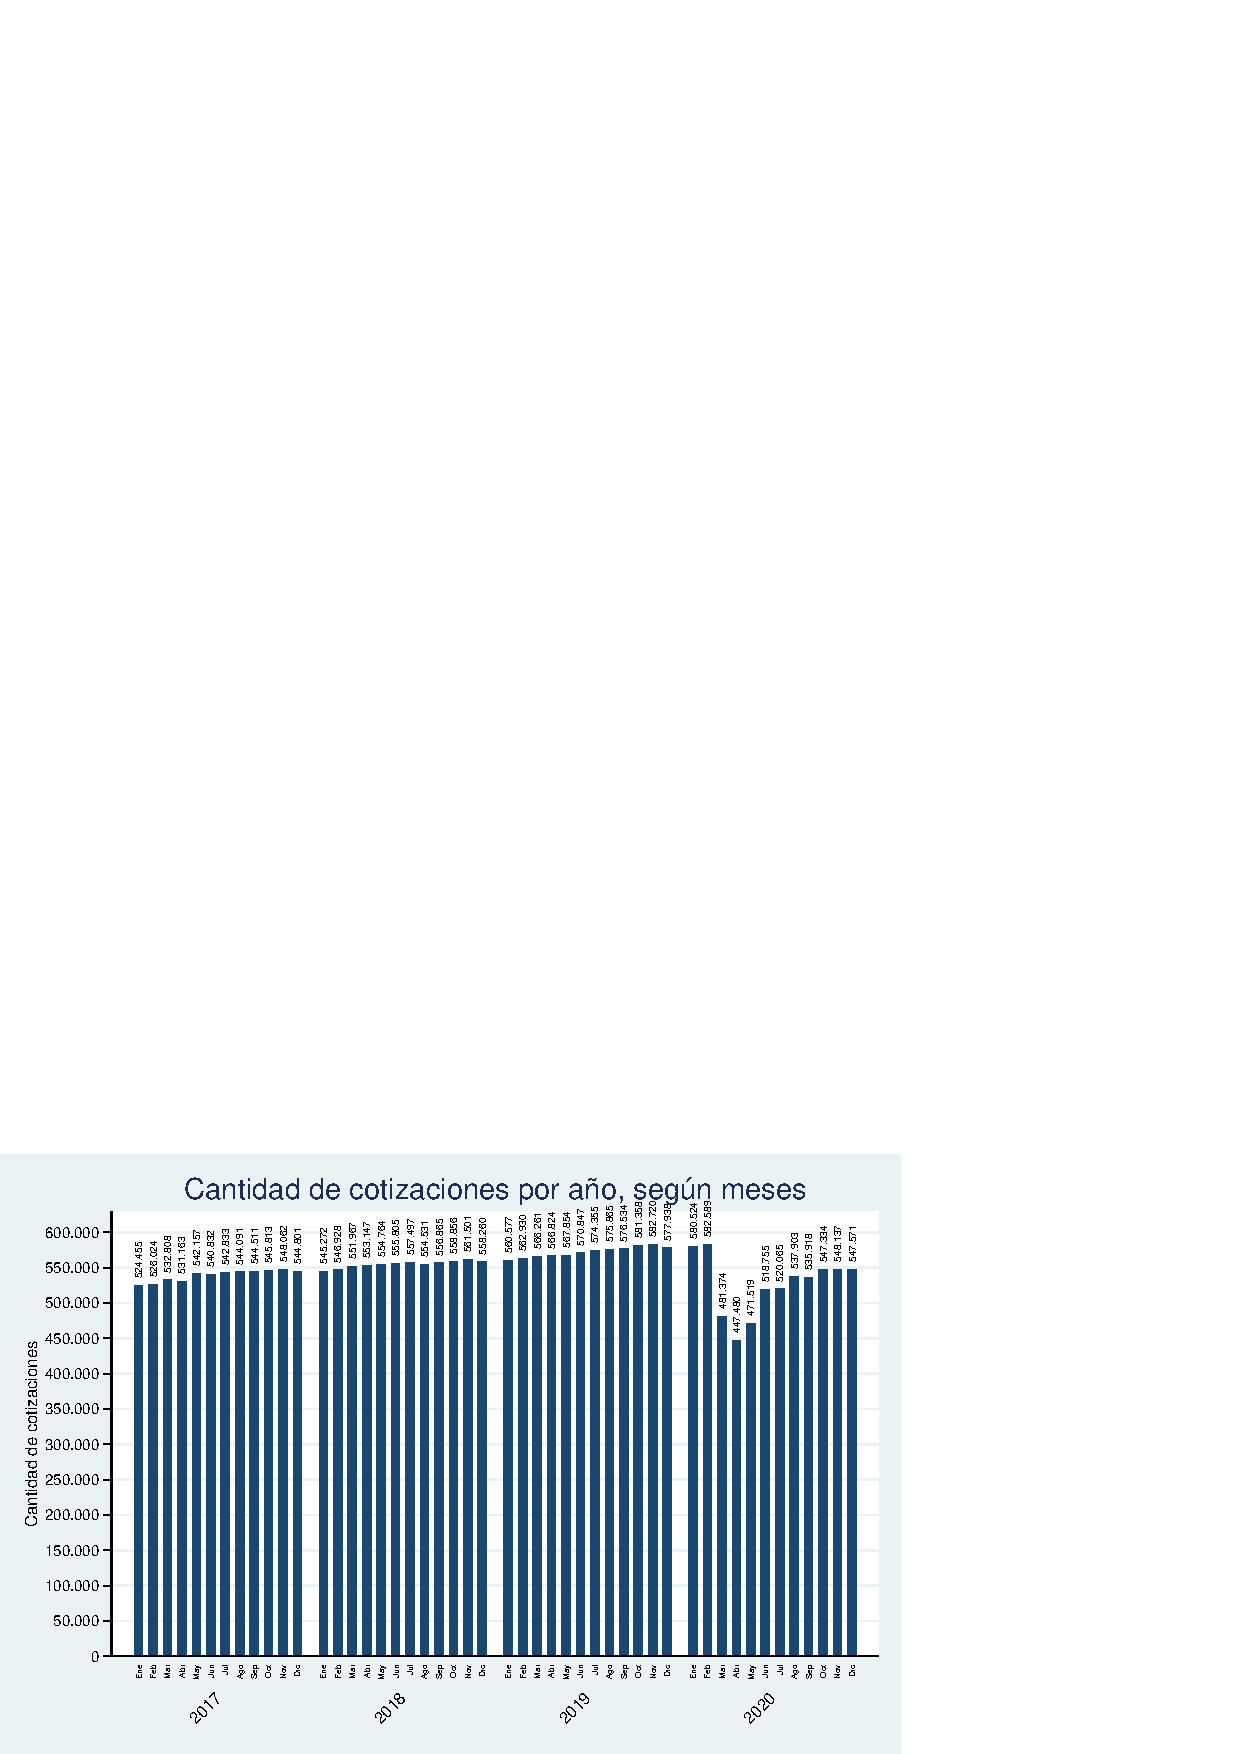
\includegraphics[scale=0.6]{RA_IPS_cotizaciones_puestos_2010a2020_mes.png}
\end{center}
\end{figure}

\begin{table}[H]
\begin{center}
\scriptsize     
\caption{\bf{Salario promedio por año y mes. (Puestos)}}
\begin{tabular}{l|rrrrrrrrrrrrr}
\input{RA_IPS_salprom_puestos_2010a2020_mes}
\end{tabular}
                    \item Fuente : Elaboración própia a partir de registros administrativos del IPS.
\end{center}
\end{table}

\begin{table}[H]
\begin{center}
\scriptsize     
\caption{\bf{Salario mediano por año y mes. (Puestos)}}
\begin{tabular}{l|rrrrrrrrrrrrr}
 & \multicolumn{13}{c}{\textbf{Mes}} \\
\textbf{Año}&\textbf{Ene}&\textbf{Feb}&\textbf{Mar}&\textbf{Abr}&\textbf{May}&\textbf{Jun}&\textbf{Jul}&\textbf{Ago}&\textbf{Sep}&\textbf{Oct}&\textbf{Nov}&\textbf{Dic}&\textbf{Total} \\
\hline
2010&1.409&1.409&1.409&1.409&1.409&1.409&1.508&1.508&1.508&1.508&1.508&1.508&1.508 \\
2011&1.508&1.508&1.508&1.658&1.658&1.658&1.658&1.658&1.658&1.658&1.658&1.658&1.658 \\
2012&1.658&1.658&1.658&1.658&1.658&1.658&1.658&1.659&1.658&1.658&1.658&1.658&1.659 \\
2013&1.658&1.658&1.658&1.658&1.659&1.658&1.659&1.659&1.659&1.659&1.658&1.658&1.659 \\
2014&1.659&1.658&1.824&1.824&1.824&1.824&1.824&1.825&1.824&1.825&1.824&1.824&1.825 \\
2015&1.824&1.824&1.824&1.824&1.825&1.825&1.825&1.825&1.825&1.825&1.824&1.824&1.825 \\
2016&1.824&1.824&1.824&1.824&1.825&1.825&1.824&1.825&1.825&1.825&1.827&1.965&1.965 \\
2017&1.965&1.965&1.978&1.978&1.985&2.000&2.042&2.061&2.044&2.052&2.050&2.066&2.066 \\
2018&2.078&2.064&2.086&2.100&2.127&2.109&2.157&2.189&2.162&2.187&2.165&2.183&2.189 \\
2019&2.187&2.163&2.197&2.200&2.222&2.200&2.254&2.270&2.253&2.268&2.250&2.259&2.270 \\
2020&2.251&2.229&2.193&2.193&2.282&2.269&2.274&2.283&2.263&2.283&2.267&2.313&2.313 \\
\textbf{Total}&2.251&2.229&2.197&2.200&2.282&2.269&2.274&2.283&2.263&2.283&2.267&2.313&2.313 \\

\end{tabular}
                    \item Fuente : Elaboración própia a partir de registros administrativos del IPS.
\end{center}
\end{table}

\begin{figure}[H]
\begin{center}
                    \caption{Salario promedio y mediano en los puestos por año y mes}
                    \vspace{0.5cm}
                    \includegraphics[scale=0.3]{RA_IPS_salprom_mediana_puestos_2010a2020_mes.png}
\end{center}
\end{figure}

\begin{table}[H]
\begin{center}
\scriptsize     
\caption{\bf{Distribución de los salarios respecto al SML (Julio de cada año)}}
\begin{tabular}{l|rrrrrrrrrrrrr}
\begin{tabular}{llllll}
\cline{1-6}
\multicolumn{1}{c}{} &
  \multicolumn{5}{|c}{Año} \\
\multicolumn{1}{c}{} &
  \multicolumn{1}{|r}{2016} &
  \multicolumn{1}{r}{2017} &
  \multicolumn{1}{r}{2018} &
  \multicolumn{1}{r}{2019} &
  \multicolumn{1}{r}{2020} \\
\cline{1-6}
\multicolumn{1}{r}{Monto del salarios nominal/SML} &
  \multicolumn{1}{|r}{} &
  \multicolumn{1}{r}{} &
  \multicolumn{1}{r}{} &
  \multicolumn{1}{r}{} &
  \multicolumn{1}{r}{} \\
\multicolumn{1}{r}{Menos de 1SML\hspace{1em}} &
  \multicolumn{1}{|r}{118.828} &
  \multicolumn{1}{r}{118.719} &
  \multicolumn{1}{r}{117.156} &
  \multicolumn{1}{r}{105.112} &
  \multicolumn{1}{r}{107.119} \\
\multicolumn{1}{r}{1 a menos de 2SML\hspace{1em}} &
  \multicolumn{1}{|r}{318.082} &
  \multicolumn{1}{r}{345.952} &
  \multicolumn{1}{r}{356.756} &
  \multicolumn{1}{r}{380.172} &
  \multicolumn{1}{r}{323.942} \\
\multicolumn{1}{r}{2 a menos de 3SML\hspace{1em}} &
  \multicolumn{1}{|r}{41.951} &
  \multicolumn{1}{r}{41.307} &
  \multicolumn{1}{r}{43.801} &
  \multicolumn{1}{r}{47.680} &
  \multicolumn{1}{r}{45.783} \\
\multicolumn{1}{r}{3 a menos de 4SML\hspace{1em}} &
  \multicolumn{1}{|r}{16.580} &
  \multicolumn{1}{r}{15.287} &
  \multicolumn{1}{r}{16.162} &
  \multicolumn{1}{r}{16.686} &
  \multicolumn{1}{r}{17.601} \\
\multicolumn{1}{r}{4 a menos de 5SML\hspace{1em}} &
  \multicolumn{1}{|r}{8.683} &
  \multicolumn{1}{r}{7.901} &
  \multicolumn{1}{r}{8.724} &
  \multicolumn{1}{r}{8.878} &
  \multicolumn{1}{r}{9.326} \\
\multicolumn{1}{r}{5 a menos de 6SML\hspace{1em}} &
  \multicolumn{1}{|r}{4.192} &
  \multicolumn{1}{r}{3.935} &
  \multicolumn{1}{r}{4.257} &
  \multicolumn{1}{r}{4.691} &
  \multicolumn{1}{r}{4.762} \\
\multicolumn{1}{r}{6 a menos de 7SML\hspace{1em}} &
  \multicolumn{1}{|r}{2.804} &
  \multicolumn{1}{r}{2.317} &
  \multicolumn{1}{r}{2.586} &
  \multicolumn{1}{r}{2.853} &
  \multicolumn{1}{r}{3.030} \\
\multicolumn{1}{r}{7 a menos de 8SML\hspace{1em}} &
  \multicolumn{1}{|r}{1.670} &
  \multicolumn{1}{r}{1.734} &
  \multicolumn{1}{r}{2.021} &
  \multicolumn{1}{r}{1.927} &
  \multicolumn{1}{r}{1.922} \\
\multicolumn{1}{r}{8 a menos de 9SML\hspace{1em}} &
  \multicolumn{1}{|r}{1.307} &
  \multicolumn{1}{r}{1.296} &
  \multicolumn{1}{r}{1.386} &
  \multicolumn{1}{r}{1.367} &
  \multicolumn{1}{r}{1.426} \\
\multicolumn{1}{r}{9 a menos de 10SML\hspace{1em}} &
  \multicolumn{1}{|r}{967} &
  \multicolumn{1}{r}{817} &
  \multicolumn{1}{r}{942} &
  \multicolumn{1}{r}{991} &
  \multicolumn{1}{r}{1.045} \\
\multicolumn{1}{r}{10SML y más\hspace{1em}} &
  \multicolumn{1}{|r}{4.101} &
  \multicolumn{1}{r}{3.568} &
  \multicolumn{1}{r}{3.706} &
  \multicolumn{1}{r}{3.998} &
  \multicolumn{1}{r}{4.109} \\
\multicolumn{1}{r}{Total\hspace{1em}} &
  \multicolumn{1}{|r}{519.165} &
  \multicolumn{1}{r}{542.833} &
  \multicolumn{1}{r}{557.497} &
  \multicolumn{1}{r}{574.355} &
  \multicolumn{1}{r}{520.065} \\
\cline{1-6}
\end{tabular}

\end{tabular}
                    \item Fuente : Elaboración própia a partir de registros administrativos del IPS.
\end{center}
\end{table}

\begin{table}[H]
\begin{center}
\scriptsize     
\caption{\bf{Distribución de los salarios respecto al SML (Julio de cada año, porcentajes)}}
\begin{tabular}{l|rrrrrrrrrrrrr}
\begin{tabular}{llllll}
\cline{1-6}
\multicolumn{1}{c}{} &
  \multicolumn{5}{|c}{Año} \\
\multicolumn{1}{c}{} &
  \multicolumn{1}{|r}{2016} &
  \multicolumn{1}{r}{2017} &
  \multicolumn{1}{r}{2018} &
  \multicolumn{1}{r}{2019} &
  \multicolumn{1}{r}{2020} \\
\cline{1-6}
\multicolumn{1}{r}{Monto del salarios nominal/SML} &
  \multicolumn{1}{|r}{} &
  \multicolumn{1}{r}{} &
  \multicolumn{1}{r}{} &
  \multicolumn{1}{r}{} &
  \multicolumn{1}{r}{} \\
\multicolumn{1}{r}{Menos de 1SML\hspace{1em}} &
  \multicolumn{1}{|r}{22,89\%} &
  \multicolumn{1}{r}{21,87\%} &
  \multicolumn{1}{r}{21,01\%} &
  \multicolumn{1}{r}{18,30\%} &
  \multicolumn{1}{r}{20,60\%} \\
\multicolumn{1}{r}{1 a menos de 2SML\hspace{1em}} &
  \multicolumn{1}{|r}{61,27\%} &
  \multicolumn{1}{r}{63,73\%} &
  \multicolumn{1}{r}{63,99\%} &
  \multicolumn{1}{r}{66,19\%} &
  \multicolumn{1}{r}{62,29\%} \\
\multicolumn{1}{r}{2 a menos de 3SML\hspace{1em}} &
  \multicolumn{1}{|r}{8,08\%} &
  \multicolumn{1}{r}{7,61\%} &
  \multicolumn{1}{r}{7,86\%} &
  \multicolumn{1}{r}{8,30\%} &
  \multicolumn{1}{r}{8,80\%} \\
\multicolumn{1}{r}{3 a menos de 4SML\hspace{1em}} &
  \multicolumn{1}{|r}{3,19\%} &
  \multicolumn{1}{r}{2,82\%} &
  \multicolumn{1}{r}{2,90\%} &
  \multicolumn{1}{r}{2,91\%} &
  \multicolumn{1}{r}{3,38\%} \\
\multicolumn{1}{r}{4 a menos de 5SML\hspace{1em}} &
  \multicolumn{1}{|r}{1,67\%} &
  \multicolumn{1}{r}{1,46\%} &
  \multicolumn{1}{r}{1,56\%} &
  \multicolumn{1}{r}{1,55\%} &
  \multicolumn{1}{r}{1,79\%} \\
\multicolumn{1}{r}{5 a menos de 6SML\hspace{1em}} &
  \multicolumn{1}{|r}{0,81\%} &
  \multicolumn{1}{r}{0,72\%} &
  \multicolumn{1}{r}{0,76\%} &
  \multicolumn{1}{r}{0,82\%} &
  \multicolumn{1}{r}{0,92\%} \\
\multicolumn{1}{r}{6 a menos de 7SML\hspace{1em}} &
  \multicolumn{1}{|r}{0,54\%} &
  \multicolumn{1}{r}{0,43\%} &
  \multicolumn{1}{r}{0,46\%} &
  \multicolumn{1}{r}{0,50\%} &
  \multicolumn{1}{r}{0,58\%} \\
\multicolumn{1}{r}{7 a menos de 8SML\hspace{1em}} &
  \multicolumn{1}{|r}{0,32\%} &
  \multicolumn{1}{r}{0,32\%} &
  \multicolumn{1}{r}{0,36\%} &
  \multicolumn{1}{r}{0,34\%} &
  \multicolumn{1}{r}{0,37\%} \\
\multicolumn{1}{r}{8 a menos de 9SML\hspace{1em}} &
  \multicolumn{1}{|r}{0,25\%} &
  \multicolumn{1}{r}{0,24\%} &
  \multicolumn{1}{r}{0,25\%} &
  \multicolumn{1}{r}{0,24\%} &
  \multicolumn{1}{r}{0,27\%} \\
\multicolumn{1}{r}{9 a menos de 10SML\hspace{1em}} &
  \multicolumn{1}{|r}{0,19\%} &
  \multicolumn{1}{r}{0,15\%} &
  \multicolumn{1}{r}{0,17\%} &
  \multicolumn{1}{r}{0,17\%} &
  \multicolumn{1}{r}{0,20\%} \\
\multicolumn{1}{r}{10SML y más\hspace{1em}} &
  \multicolumn{1}{|r}{0,79\%} &
  \multicolumn{1}{r}{0,66\%} &
  \multicolumn{1}{r}{0,66\%} &
  \multicolumn{1}{r}{0,70\%} &
  \multicolumn{1}{r}{0,79\%} \\
\multicolumn{1}{r}{Total\hspace{1em}} &
  \multicolumn{1}{|r}{100,00\%} &
  \multicolumn{1}{r}{100,00\%} &
  \multicolumn{1}{r}{100,00\%} &
  \multicolumn{1}{r}{100,00\%} &
  \multicolumn{1}{r}{100,00\%} \\
\cline{1-6}
\end{tabular}

\end{tabular}
                    \item Fuente : Elaboración própia a partir de registros administrativos del IPS.
\end{center}
\end{table}

\begin{figure}[H]
\begin{center}
                    \caption{Distribución de los salarios respecto al SML (Julio de cada año, porcentajes)}
                    \vspace{0.5cm}
                    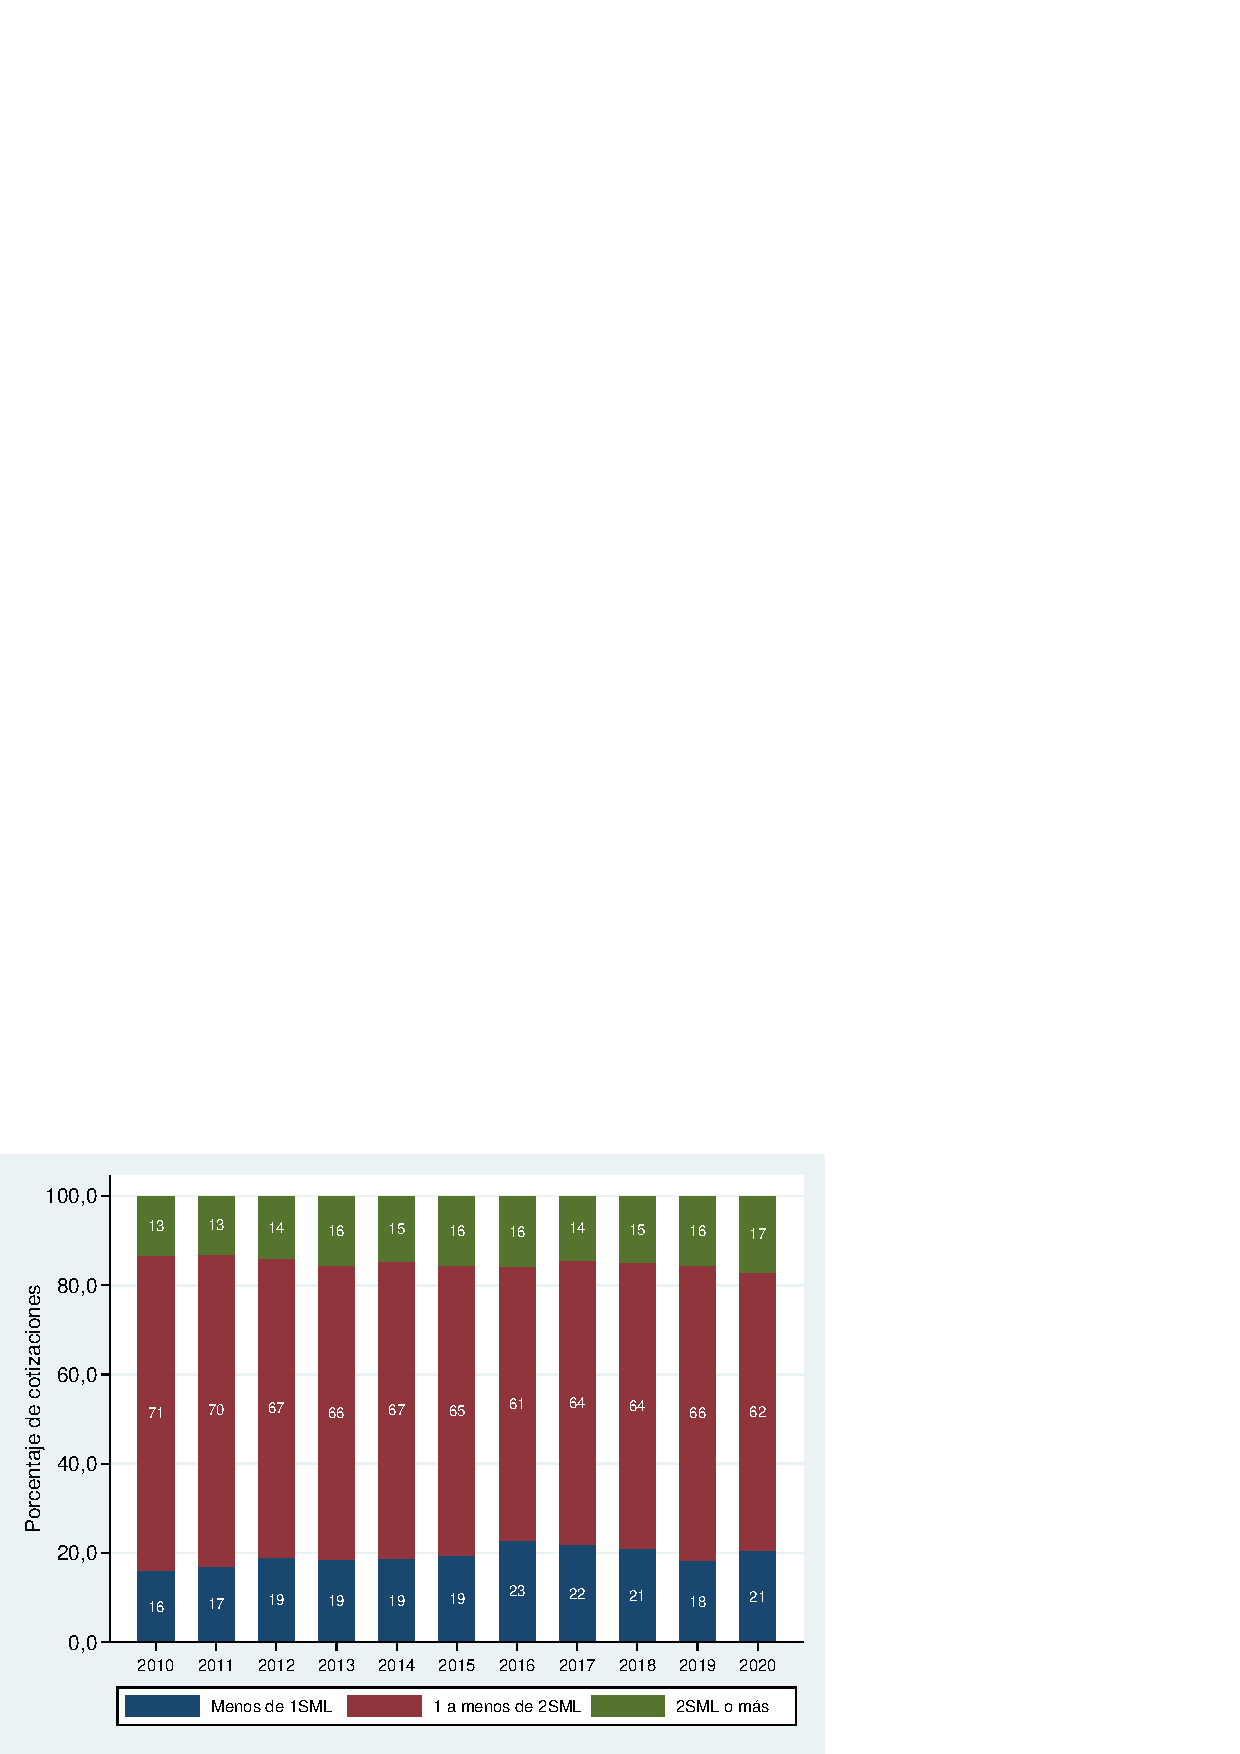
\includegraphics[scale=0.6]{RA_IPS_dist_salarial_puestos_2010a2020_mes_porcentajes.png}
\end{center}
\end{figure}

\begin{table}[H]
\begin{center}
\scriptsize     
\caption{\bf{Cantidad de cotizaciones por tipo de seguro y año (Julio de cada año, cantidades)}}
\begin{tabular}{l|rrrrrrrrrrrrr}
\begin{tabular}{lllllllll}
\cline{1-9}
\multicolumn{1}{c}{} &
  \multicolumn{8}{|c}{Año} \\
\multicolumn{1}{c}{} &
  \multicolumn{1}{|r}{2013} &
  \multicolumn{1}{r}{2014} &
  \multicolumn{1}{r}{2015} &
  \multicolumn{1}{r}{2016} &
  \multicolumn{1}{r}{2017} &
  \multicolumn{1}{r}{2018} &
  \multicolumn{1}{r}{2019} &
  \multicolumn{1}{r}{2020} \\
\cline{1-9}
\multicolumn{1}{l}{Tipo de seguro en el puesto} &
  \multicolumn{1}{|r}{} &
  \multicolumn{1}{r}{} &
  \multicolumn{1}{r}{} &
  \multicolumn{1}{r}{} &
  \multicolumn{1}{r}{} &
  \multicolumn{1}{r}{} &
  \multicolumn{1}{r}{} &
  \multicolumn{1}{r}{} \\
\multicolumn{1}{l}{\hspace{1em}Ama de Casa} &
  \multicolumn{1}{|r}{} &
  \multicolumn{1}{r}{43} &
  \multicolumn{1}{r}{83} &
  \multicolumn{1}{r}{89} &
  \multicolumn{1}{r}{94} &
  \multicolumn{1}{r}{94} &
  \multicolumn{1}{r}{88} &
  \multicolumn{1}{r}{76} \\
\multicolumn{1}{l}{\hspace{1em}Aprendices} &
  \multicolumn{1}{|r}{725} &
  \multicolumn{1}{r}{1.220} &
  \multicolumn{1}{r}{1.988} &
  \multicolumn{1}{r}{1.776} &
  \multicolumn{1}{r}{1.997} &
  \multicolumn{1}{r}{2.303} &
  \multicolumn{1}{r}{2.905} &
  \multicolumn{1}{r}{2.064} \\
\multicolumn{1}{l}{\hspace{1em}Continuidad en el Beneficio} &
  \multicolumn{1}{|r}{1.311} &
  \multicolumn{1}{r}{1.857} &
  \multicolumn{1}{r}{1.998} &
  \multicolumn{1}{r}{1.969} &
  \multicolumn{1}{r}{2.032} &
  \multicolumn{1}{r}{1.984} &
  \multicolumn{1}{r}{1.830} &
  \multicolumn{1}{r}{1.521} \\
\multicolumn{1}{l}{\hspace{1em}Chofer Cobrador} &
  \multicolumn{1}{|r}{645} &
  \multicolumn{1}{r}{665} &
  \multicolumn{1}{r}{853} &
  \multicolumn{1}{r}{1.195} &
  \multicolumn{1}{r}{1.189} &
  \multicolumn{1}{r}{1.289} &
  \multicolumn{1}{r}{1.318} &
  \multicolumn{1}{r}{1.028} \\
\multicolumn{1}{l}{\hspace{1em}Cotizante General} &
  \multicolumn{1}{|r}{320.164} &
  \multicolumn{1}{r}{342.603} &
  \multicolumn{1}{r}{360.068} &
  \multicolumn{1}{r}{372.044} &
  \multicolumn{1}{r}{395.870} &
  \multicolumn{1}{r}{412.060} &
  \multicolumn{1}{r}{424.563} &
  \multicolumn{1}{r}{381.110} \\
\multicolumn{1}{l}{\hspace{1em}Chofer de Omnibus} &
  \multicolumn{1}{|r}{571} &
  \multicolumn{1}{r}{677} &
  \multicolumn{1}{r}{665} &
  \multicolumn{1}{r}{719} &
  \multicolumn{1}{r}{693} &
  \multicolumn{1}{r}{643} &
  \multicolumn{1}{r}{633} &
  \multicolumn{1}{r}{384} \\
\multicolumn{1}{l}{\hspace{1em}Chofer a Inconstitucionalidad} &
  \multicolumn{1}{|r}{2.639} &
  \multicolumn{1}{r}{1.998} &
  \multicolumn{1}{r}{2.088} &
  \multicolumn{1}{r}{1.737} &
  \multicolumn{1}{r}{1.579} &
  \multicolumn{1}{r}{1.343} &
  \multicolumn{1}{r}{1.274} &
  \multicolumn{1}{r}{1.066} \\
\multicolumn{1}{l}{\hspace{1em}Jornalero a Destajo} &
  \multicolumn{1}{|r}{62.299} &
  \multicolumn{1}{r}{67.322} &
  \multicolumn{1}{r}{71.473} &
  \multicolumn{1}{r}{79.853} &
  \multicolumn{1}{r}{80.733} &
  \multicolumn{1}{r}{81.051} &
  \multicolumn{1}{r}{84.095} &
  \multicolumn{1}{r}{79.548} \\
\multicolumn{1}{l}{\hspace{1em}Cotizante Zafrero} &
  \multicolumn{1}{|r}{1.157} &
  \multicolumn{1}{r}{1.832} &
  \multicolumn{1}{r}{2.589} &
  \multicolumn{1}{r}{2.631} &
  \multicolumn{1}{r}{2.979} &
  \multicolumn{1}{r}{3.287} &
  \multicolumn{1}{r}{3.516} &
  \multicolumn{1}{r}{3.607} \\
\multicolumn{1}{l}{\hspace{1em}Doméstico Independiente} &
  \multicolumn{1}{|r}{} &
  \multicolumn{1}{r}{104} &
  \multicolumn{1}{r}{128} &
  \multicolumn{1}{r}{} &
  \multicolumn{1}{r}{} &
  \multicolumn{1}{r}{} &
  \multicolumn{1}{r}{} &
  \multicolumn{1}{r}{} \\
\multicolumn{1}{l}{\hspace{1em}Estibador Marítimo} &
  \multicolumn{1}{|r}{217} &
  \multicolumn{1}{r}{225} &
  \multicolumn{1}{r}{193} &
  \multicolumn{1}{r}{209} &
  \multicolumn{1}{r}{302} &
  \multicolumn{1}{r}{251} &
  \multicolumn{1}{r}{262} &
  \multicolumn{1}{r}{334} \\
\multicolumn{1}{l}{\hspace{1em}Empleadores} &
  \multicolumn{1}{|r}{} &
  \multicolumn{1}{r}{10} &
  \multicolumn{1}{r}{14} &
  \multicolumn{1}{r}{12} &
  \multicolumn{1}{r}{13} &
  \multicolumn{1}{r}{13} &
  \multicolumn{1}{r}{14} &
  \multicolumn{1}{r}{14} \\
\multicolumn{1}{l}{\hspace{1em}Ganadero tipo A} &
  \multicolumn{1}{|r}{8.454} &
  \multicolumn{1}{r}{8.783} &
  \multicolumn{1}{r}{9.148} &
  \multicolumn{1}{r}{9.443} &
  \multicolumn{1}{r}{9.270} &
  \multicolumn{1}{r}{8.735} &
  \multicolumn{1}{r}{9.140} &
  \multicolumn{1}{r}{8.876} \\
\multicolumn{1}{l}{\hspace{1em}Ganadero tipo B} &
  \multicolumn{1}{|r}{9.168} &
  \multicolumn{1}{r}{9.469} &
  \multicolumn{1}{r}{9.542} &
  \multicolumn{1}{r}{9.681} &
  \multicolumn{1}{r}{10.019} &
  \multicolumn{1}{r}{9.975} &
  \multicolumn{1}{r}{10.372} &
  \multicolumn{1}{r}{10.224} \\
\multicolumn{1}{l}{\hspace{1em}Cobrador y/o guarda} &
  \multicolumn{1}{|r}{100} &
  \multicolumn{1}{r}{125} &
  \multicolumn{1}{r}{122} &
  \multicolumn{1}{r}{142} &
  \multicolumn{1}{r}{128} &
  \multicolumn{1}{r}{108} &
  \multicolumn{1}{r}{101} &
  \multicolumn{1}{r}{52} \\
\multicolumn{1}{l}{\hspace{1em}Menores y Aprendices} &
  \multicolumn{1}{|r}{857} &
  \multicolumn{1}{r}{72} &
  \multicolumn{1}{r}{} &
  \multicolumn{1}{r}{} &
  \multicolumn{1}{r}{} &
  \multicolumn{1}{r}{} &
  \multicolumn{1}{r}{} &
  \multicolumn{1}{r}{} \\
\multicolumn{1}{l}{\hspace{1em}Menores} &
  \multicolumn{1}{|r}{101} &
  \multicolumn{1}{r}{196} &
  \multicolumn{1}{r}{174} &
  \multicolumn{1}{r}{120} &
  \multicolumn{1}{r}{123} &
  \multicolumn{1}{r}{106} &
  \multicolumn{1}{r}{84} &
  \multicolumn{1}{r}{74} \\
\multicolumn{1}{l}{\hspace{1em}Magisterio Privado} &
  \multicolumn{1}{|r}{17.701} &
  \multicolumn{1}{r}{17.849} &
  \multicolumn{1}{r}{18.163} &
  \multicolumn{1}{r}{18.316} &
  \multicolumn{1}{r}{18.108} &
  \multicolumn{1}{r}{18.038} &
  \multicolumn{1}{r}{18.663} &
  \multicolumn{1}{r}{15.437} \\
\multicolumn{1}{l}{\hspace{1em}Propietarios} &
  \multicolumn{1}{|r}{} &
  \multicolumn{1}{r}{5} &
  \multicolumn{1}{r}{7} &
  \multicolumn{1}{r}{7} &
  \multicolumn{1}{r}{8} &
  \multicolumn{1}{r}{10} &
  \multicolumn{1}{r}{12} &
  \multicolumn{1}{r}{9} \\
\multicolumn{1}{l}{\hspace{1em}Representantes del Empleador} &
  \multicolumn{1}{|r}{} &
  \multicolumn{1}{r}{5} &
  \multicolumn{1}{r}{6} &
  \multicolumn{1}{r}{7} &
  \multicolumn{1}{r}{10} &
  \multicolumn{1}{r}{8} &
  \multicolumn{1}{r}{9} &
  \multicolumn{1}{r}{11} \\
\multicolumn{1}{l}{\hspace{1em}Seguro Doméstico} &
  \multicolumn{1}{|r}{} &
  \multicolumn{1}{r}{} &
  \multicolumn{1}{r}{} &
  \multicolumn{1}{r}{18.889} &
  \multicolumn{1}{r}{17.319} &
  \multicolumn{1}{r}{15.827} &
  \multicolumn{1}{r}{15.148} &
  \multicolumn{1}{r}{8.679} \\
\multicolumn{1}{l}{\hspace{1em}Trabajadores Independientes} &
  \multicolumn{1}{|r}{} &
  \multicolumn{1}{r}{181} &
  \multicolumn{1}{r}{276} &
  \multicolumn{1}{r}{326} &
  \multicolumn{1}{r}{367} &
  \multicolumn{1}{r}{372} &
  \multicolumn{1}{r}{328} &
  \multicolumn{1}{r}{310} \\
\multicolumn{1}{l}{\hspace{1em}Tiempo Parcial} &
  \multicolumn{1}{|r}{} &
  \multicolumn{1}{r}{} &
  \multicolumn{1}{r}{} &
  \multicolumn{1}{r}{} &
  \multicolumn{1}{r}{} &
  \multicolumn{1}{r}{} &
  \multicolumn{1}{r}{} &
  \multicolumn{1}{r}{5.641} \\
\multicolumn{1}{l}{\hspace{1em}Total} &
  \multicolumn{1}{|r}{426.109} &
  \multicolumn{1}{r}{455.241} &
  \multicolumn{1}{r}{479.578} &
  \multicolumn{1}{r}{519.165} &
  \multicolumn{1}{r}{542.833} &
  \multicolumn{1}{r}{557.497} &
  \multicolumn{1}{r}{574.355} &
  \multicolumn{1}{r}{520.065} \\
\cline{1-9}
\end{tabular}

\end{tabular}
                    \item Fuente : Elaboración própia a partir de registros administrativos del IPS.
\end{center}
\end{table}

\begin{table}[H]
\begin{center}
\scriptsize     
\caption{\bf{Salario promedio por tipo de seguro y año (Julio de cada año, porcentajes)}}
\begin{tabular}{l|rrrrrrrrrrrrr}
\begin{tabular}{lllllllll}
\cline{1-9}
\multicolumn{1}{c}{} &
  \multicolumn{8}{|c}{Año} \\
\multicolumn{1}{c}{} &
  \multicolumn{1}{|r}{2013} &
  \multicolumn{1}{r}{2014} &
  \multicolumn{1}{r}{2015} &
  \multicolumn{1}{r}{2016} &
  \multicolumn{1}{r}{2017} &
  \multicolumn{1}{r}{2018} &
  \multicolumn{1}{r}{2019} &
  \multicolumn{1}{r}{2020} \\
\cline{1-9}
\multicolumn{1}{l}{Tipo de seguro en el puesto} &
  \multicolumn{1}{|r}{} &
  \multicolumn{1}{r}{} &
  \multicolumn{1}{r}{} &
  \multicolumn{1}{r}{} &
  \multicolumn{1}{r}{} &
  \multicolumn{1}{r}{} &
  \multicolumn{1}{r}{} &
  \multicolumn{1}{r}{} \\
\multicolumn{1}{l}{\hspace{1em}Ama de Casa} &
  \multicolumn{1}{|r}{} &
  \multicolumn{1}{r}{1.735.470} &
  \multicolumn{1}{r}{1.903.943} &
  \multicolumn{1}{r}{1.949.047} &
  \multicolumn{1}{r}{2.136.054} &
  \multicolumn{1}{r}{2.233.392} &
  \multicolumn{1}{r}{2.285.286} &
  \multicolumn{1}{r}{2.235.240} \\
\multicolumn{1}{l}{\hspace{1em}Aprendices} &
  \multicolumn{1}{|r}{1.653.246} &
  \multicolumn{1}{r}{1.575.525} &
  \multicolumn{1}{r}{1.573.089} &
  \multicolumn{1}{r}{1.388.009} &
  \multicolumn{1}{r}{1.656.406} &
  \multicolumn{1}{r}{1.879.165} &
  \multicolumn{1}{r}{1.938.421} &
  \multicolumn{1}{r}{2.137.402} \\
\multicolumn{1}{l}{\hspace{1em}Continuidad en el Beneficio} &
  \multicolumn{1}{|r}{3.249.500} &
  \multicolumn{1}{r}{3.414.139} &
  \multicolumn{1}{r}{3.546.595} &
  \multicolumn{1}{r}{3.812.223} &
  \multicolumn{1}{r}{4.130.066} &
  \multicolumn{1}{r}{4.548.354} &
  \multicolumn{1}{r}{4.898.909} &
  \multicolumn{1}{r}{4.892.697} \\
\multicolumn{1}{l}{\hspace{1em}Chofer Cobrador} &
  \multicolumn{1}{|r}{2.160.019} &
  \multicolumn{1}{r}{2.482.627} &
  \multicolumn{1}{r}{2.233.969} &
  \multicolumn{1}{r}{2.179.651} &
  \multicolumn{1}{r}{2.451.680} &
  \multicolumn{1}{r}{2.446.201} &
  \multicolumn{1}{r}{2.661.264} &
  \multicolumn{1}{r}{2.786.482} \\
\multicolumn{1}{l}{\hspace{1em}Cotizante General} &
  \multicolumn{1}{|r}{2.875.762} &
  \multicolumn{1}{r}{3.059.070} &
  \multicolumn{1}{r}{3.133.589} &
  \multicolumn{1}{r}{3.180.374} &
  \multicolumn{1}{r}{3.398.489} &
  \multicolumn{1}{r}{3.540.629} &
  \multicolumn{1}{r}{3.685.888} &
  \multicolumn{1}{r}{3.839.875} \\
\multicolumn{1}{l}{\hspace{1em}Chofer de Omnibus} &
  \multicolumn{1}{|r}{2.218.842} &
  \multicolumn{1}{r}{2.434.335} &
  \multicolumn{1}{r}{2.307.428} &
  \multicolumn{1}{r}{2.251.718} &
  \multicolumn{1}{r}{2.614.291} &
  \multicolumn{1}{r}{2.722.769} &
  \multicolumn{1}{r}{2.727.145} &
  \multicolumn{1}{r}{2.568.566} \\
\multicolumn{1}{l}{\hspace{1em}Chofer a Inconstitucionalidad} &
  \multicolumn{1}{|r}{2.078.803} &
  \multicolumn{1}{r}{2.353.808} &
  \multicolumn{1}{r}{2.229.077} &
  \multicolumn{1}{r}{2.147.926} &
  \multicolumn{1}{r}{2.398.288} &
  \multicolumn{1}{r}{2.493.070} &
  \multicolumn{1}{r}{2.768.052} &
  \multicolumn{1}{r}{2.573.789} \\
\multicolumn{1}{l}{\hspace{1em}Jornalero a Destajo} &
  \multicolumn{1}{|r}{1.754.919} &
  \multicolumn{1}{r}{1.858.612} &
  \multicolumn{1}{r}{1.864.311} &
  \multicolumn{1}{r}{1.867.158} &
  \multicolumn{1}{r}{2.087.503} &
  \multicolumn{1}{r}{2.229.835} &
  \multicolumn{1}{r}{2.279.792} &
  \multicolumn{1}{r}{2.313.656} \\
\multicolumn{1}{l}{\hspace{1em}Cotizante Zafrero} &
  \multicolumn{1}{|r}{2.054.868} &
  \multicolumn{1}{r}{2.062.367} &
  \multicolumn{1}{r}{2.204.650} &
  \multicolumn{1}{r}{2.459.558} &
  \multicolumn{1}{r}{2.802.903} &
  \multicolumn{1}{r}{2.694.971} &
  \multicolumn{1}{r}{2.905.446} &
  \multicolumn{1}{r}{2.766.485} \\
\multicolumn{1}{l}{\hspace{1em}Doméstico Independiente} &
  \multicolumn{1}{|r}{} &
  \multicolumn{1}{r}{778.525} &
  \multicolumn{1}{r}{801.069} &
  \multicolumn{1}{r}{} &
  \multicolumn{1}{r}{} &
  \multicolumn{1}{r}{} &
  \multicolumn{1}{r}{} &
  \multicolumn{1}{r}{} \\
\multicolumn{1}{l}{\hspace{1em}Estibador Marítimo} &
  \multicolumn{1}{|r}{702.527} &
  \multicolumn{1}{r}{720.739} &
  \multicolumn{1}{r}{755.431} &
  \multicolumn{1}{r}{749.536} &
  \multicolumn{1}{r}{1.679.438} &
  \multicolumn{1}{r}{2.159.302} &
  \multicolumn{1}{r}{1.176.313} &
  \multicolumn{1}{r}{1.115.608} \\
\multicolumn{1}{l}{\hspace{1em}Empleadores} &
  \multicolumn{1}{|r}{} &
  \multicolumn{1}{r}{1.942.244} &
  \multicolumn{1}{r}{2.818.752} &
  \multicolumn{1}{r}{3.282.152} &
  \multicolumn{1}{r}{3.609.252} &
  \multicolumn{1}{r}{3.590.446} &
  \multicolumn{1}{r}{3.547.957} &
  \multicolumn{1}{r}{2.492.192} \\
\multicolumn{1}{l}{\hspace{1em}Ganadero tipo A} &
  \multicolumn{1}{|r}{886.932} &
  \multicolumn{1}{r}{988.015} &
  \multicolumn{1}{r}{1.012.503} &
  \multicolumn{1}{r}{1.051.347} &
  \multicolumn{1}{r}{1.197.540} &
  \multicolumn{1}{r}{1.292.081} &
  \multicolumn{1}{r}{1.358.716} &
  \multicolumn{1}{r}{1.393.903} \\
\multicolumn{1}{l}{\hspace{1em}Ganadero tipo B} &
  \multicolumn{1}{|r}{1.475.131} &
  \multicolumn{1}{r}{1.624.327} &
  \multicolumn{1}{r}{1.670.776} &
  \multicolumn{1}{r}{1.741.572} &
  \multicolumn{1}{r}{1.841.931} &
  \multicolumn{1}{r}{2.008.215} &
  \multicolumn{1}{r}{2.104.973} &
  \multicolumn{1}{r}{2.150.600} \\
\multicolumn{1}{l}{\hspace{1em}Cobrador y/o guarda} &
  \multicolumn{1}{|r}{2.007.971} &
  \multicolumn{1}{r}{2.223.846} &
  \multicolumn{1}{r}{2.044.764} &
  \multicolumn{1}{r}{2.035.331} &
  \multicolumn{1}{r}{2.106.061} &
  \multicolumn{1}{r}{2.199.516} &
  \multicolumn{1}{r}{2.200.121} &
  \multicolumn{1}{r}{2.057.306} \\
\multicolumn{1}{l}{\hspace{1em}Menores y Aprendices} &
  \multicolumn{1}{|r}{1.129.532} &
  \multicolumn{1}{r}{1.596.349} &
  \multicolumn{1}{r}{} &
  \multicolumn{1}{r}{} &
  \multicolumn{1}{r}{} &
  \multicolumn{1}{r}{} &
  \multicolumn{1}{r}{} &
  \multicolumn{1}{r}{} \\
\multicolumn{1}{l}{\hspace{1em}Menores} &
  \multicolumn{1}{|r}{1.288.099} &
  \multicolumn{1}{r}{1.252.958} &
  \multicolumn{1}{r}{1.343.236} &
  \multicolumn{1}{r}{1.338.902} &
  \multicolumn{1}{r}{1.534.888} &
  \multicolumn{1}{r}{1.793.026} &
  \multicolumn{1}{r}{1.989.599} &
  \multicolumn{1}{r}{2.148.239} \\
\multicolumn{1}{l}{\hspace{1em}Magisterio Privado} &
  \multicolumn{1}{|r}{1.601.994} &
  \multicolumn{1}{r}{1.703.522} &
  \multicolumn{1}{r}{1.766.080} &
  \multicolumn{1}{r}{1.875.243} &
  \multicolumn{1}{r}{2.026.646} &
  \multicolumn{1}{r}{2.200.610} &
  \multicolumn{1}{r}{2.379.327} &
  \multicolumn{1}{r}{2.478.946} \\
\multicolumn{1}{l}{\hspace{1em}Propietarios} &
  \multicolumn{1}{|r}{} &
  \multicolumn{1}{r}{1.859.244} &
  \multicolumn{1}{r}{1.597.297} &
  \multicolumn{1}{r}{1.849.190} &
  \multicolumn{1}{r}{2.041.123} &
  \multicolumn{1}{r}{2.240.050} &
  \multicolumn{1}{r}{2.285.699} &
  \multicolumn{1}{r}{2.254.746} \\
\multicolumn{1}{l}{\hspace{1em}Representantes del Empleador} &
  \multicolumn{1}{|r}{} &
  \multicolumn{1}{r}{2.337.640} &
  \multicolumn{1}{r}{3.412.028} &
  \multicolumn{1}{r}{3.037.513} &
  \multicolumn{1}{r}{4.480.562} &
  \multicolumn{1}{r}{4.009.101} &
  \multicolumn{1}{r}{6.991.219} &
  \multicolumn{1}{r}{6.118.787} \\
\multicolumn{1}{l}{\hspace{1em}Seguro Doméstico} &
  \multicolumn{1}{|r}{} &
  \multicolumn{1}{r}{} &
  \multicolumn{1}{r}{} &
  \multicolumn{1}{r}{1.096.934} &
  \multicolumn{1}{r}{1.239.628} &
  \multicolumn{1}{r}{1.288.513} &
  \multicolumn{1}{r}{2.141.098} &
  \multicolumn{1}{r}{2.183.722} \\
\multicolumn{1}{l}{\hspace{1em}Trabajadores Independientes} &
  \multicolumn{1}{|r}{} &
  \multicolumn{1}{r}{1.885.546} &
  \multicolumn{1}{r}{2.039.887} &
  \multicolumn{1}{r}{2.053.929} &
  \multicolumn{1}{r}{2.515.378} &
  \multicolumn{1}{r}{2.636.275} &
  \multicolumn{1}{r}{3.108.561} &
  \multicolumn{1}{r}{3.016.326} \\
\multicolumn{1}{l}{\hspace{1em}Tiempo Parcial} &
  \multicolumn{1}{|r}{} &
  \multicolumn{1}{r}{} &
  \multicolumn{1}{r}{} &
  \multicolumn{1}{r}{} &
  \multicolumn{1}{r}{} &
  \multicolumn{1}{r}{} &
  \multicolumn{1}{r}{} &
  \multicolumn{1}{r}{1.184.705} \\
\multicolumn{1}{l}{\hspace{1em}Total} &
  \multicolumn{1}{|r}{2.574.125} &
  \multicolumn{1}{r}{2.743.639} &
  \multicolumn{1}{r}{2.803.244} &
  \multicolumn{1}{r}{2.773.901} &
  \multicolumn{1}{r}{3.007.139} &
  \multicolumn{1}{r}{3.163.804} &
  \multicolumn{1}{r}{3.313.859} &
  \multicolumn{1}{r}{3.414.990} \\
\cline{1-9}
\end{tabular}

\end{tabular}
                    \item Fuente : Elaboración própia a partir de registros administrativos del IPS.
\end{center}
\end{table}
